\documentclass[a4paper]{article}
\usepackage[utf8]{inputenc}
\usepackage{vntex}
%\usepackage[english,vietnam]{babel}

%\usepackage[utf8]{inputenc}
%\usepackage[francais]{babel}
\usepackage{a4wide,amssymb,epsfig,latexsym,multicol,array,hhline,fancyhdr}
\usepackage{booktabs}
\usepackage{amsmath}
\usepackage{lastpage}
\usepackage[lined,boxed,commentsnumbered]{algorithm2e}
\usepackage{enumerate}
\usepackage{color}
\usepackage{graphicx}							% Standard graphics package
\usepackage{array}
\usepackage{tabularx, caption}
\usepackage{longtable}
\usepackage{float}
\usepackage{multirow}
\usepackage[framemethod=tikz]{mdframed}% For highlighting paragraph backgrounds
\usepackage{multicol}
\usepackage{rotating}
\usepackage{graphics}
\usepackage[a4paper, left=2.5cm, right=2cm, top=2.5cm, bottom=2.5cm, headheight=30pt, headsep=10pt]{geometry}\usepackage{setspace}
\usepackage{epsfig}
\usepackage{tikz}
\usepackage{listings}
\usetikzlibrary{arrows,snakes,backgrounds}
\usepackage{hyperref}
\hypersetup{urlcolor=blue,linkcolor=black,citecolor=black,colorlinks=true} 
%\usepackage{pstcol} 								% PSTricks with the standard color package

\renewcommand{\topfraction}{0.9}
\renewcommand{\bottomfraction}{0.8}
\renewcommand{\textfraction}{0.1}
\renewcommand{\floatpagefraction}{0.8}

\newtheorem{theorem}{{\bf Định lý}}
\newtheorem{property}{{\bf Tính chất}}
\newtheorem{proposition}{{\bf Mệnh đề}}
\newtheorem{corollary}[proposition]{{\bf Hệ quả}}
\newtheorem{lemma}[proposition]{{\bf Bổ đề}}

\everymath{\color{black}}
%\usepackage{fancyhdr}
\setlength{\headheight}{40pt}
\pagestyle{fancy}
\fancyhead{} % clear all header fields
\fancyhead[L]{
 \begin{tabular}{rl}
    \begin{picture}(25,15)(0,0)
    \put(0,-8){
\includegraphics[width=8mm, height=8mm]{hcmut.png}}
    %\put(0,-8){\epsfig{width=10mm,figure=hcmut.eps}}
   \end{picture}&
	%
\includegraphics[width=8mm, height=8mm]{hcmut.png} & %
	\begin{tabular}{l}
		\textbf{\bf \ttfamily Trường Đại Học Bách Khoa Tp.Hồ Chí Minh}\\
		\textbf{\bf \ttfamily Khoa Khoa Học và Kỹ Thuật Máy Tính}
	\end{tabular} 	
 \end{tabular}
}
\fancyhead[R]{
	\begin{tabular}{l}
		\tiny \bf \\
		\tiny \bf 
	\end{tabular}  }
\fancyfoot{} % clear all footer fields
\fancyfoot[L]{\scriptsize \ttfamily Bài tập lớn môn Kho dữ liệu và Hệ hỗ trợ Quyết định - Niên khóa 2026-2027}
\fancyfoot[R]{\scriptsize \ttfamily Trang {\thepage}/\pageref{LastPage}}
\renewcommand{\headrulewidth}{0.3pt}
\renewcommand{\footrulewidth}{0.3pt}


%%%
\setcounter{secnumdepth}{4}
\setcounter{tocdepth}{3}
\makeatletter
\newcounter {subsubsubsection}[subsubsection]
\renewcommand\thesubsubsubsection{\thesubsubsection .\@alph\c@subsubsubsection}
\newcommand\subsubsubsection{\@startsection{subsubsubsection}{4}{\z@}%
                                     {-3.25ex\@plus -1ex \@minus -.2ex}%
                                     {1.5ex \@plus .2ex}%
                                     {\normalfont\normalsize\bfseries}}
\newcommand*\l@subsubsubsection{\@dottedtocline{3}{10.0em}{4.1em}}
\newcommand*{\subsubsubsectionmark}[1]{}
\makeatother

\definecolor{dkgreen}{rgb}{0,0.6,0}
\definecolor{gray}{rgb}{0.5,0.5,0.5}
\definecolor{mauve}{rgb}{0.58,0,0.82}

\lstset{frame=tb,
	language=SQL,
	aboveskip=3mm,
	belowskip=3mm,
	showstringspaces=false,
	columns=flexible,
	basicstyle={\small\ttfamily},
	numbers=none,
	numberstyle=\tiny\color{gray},
	keywordstyle=\color{blue},
	commentstyle=\color{dkgreen},
	stringstyle=\color{mauve},
	breaklines=true,
	breakatwhitespace=true,
	tabsize=3,
	numbers=left,
	stepnumber=1,
	numbersep=1pt,    
	firstnumber=1,
	numberfirstline=true
}

\begin{document}

\begin{titlepage}
\thispagestyle{empty}
\everymath{}%
\color{black}%
\definecolor{accent}{HTML}{333333}%
\centering

{\large
ĐẠI HỌC QUỐC GIA TP.HCM \\
TRƯỜNG ĐẠI HỌC BÁCH KHOA \\
KHOA KHOA HỌC VÀ KỸ THUẬT MÁY TÍNH\par
}

\vspace{1.2cm}


\includegraphics[width=10cm]{hcmut.png}\par

\vspace{1.2cm}

{\large\bfseries KHO DỮ LIỆU VÀ HỆ HỖ TRỢ QUYẾT ĐỊNH (CO4031) -- HK261\par}
\smallskip
{\large BÁO CÁO BÀI TẬP LỚN\par}

\vspace{1.2cm}

{\color{accent}\rule{\linewidth}{0.8pt}}\par
\medskip
\parbox{\linewidth}{\centering
{\LARGE\bfseries HỆ HỖ TRỢ QUYẾT ĐỊNH CAN THIỆP \\ NGƯỜI BÁN TRÊN SÀN OLIST\par}
\smallskip
{\large\itshape Từ kho dữ liệu đến lựa chọn chính sách\par}
}\par
\medskip
{\color{accent}\rule{\linewidth}{0.8pt}}\par

\vspace{1.2cm}

\begin{tabular}{@{}l@{\hspace{1em}}l@{\hspace{1.5em}}r@{}}
\textbf{GVHD:} & Đỗ Thanh Thái & \\
\textbf{Nhóm:} & 18 & \\
\textbf{Sinh viên thực hiện:} & Nguyễn Đức Toàn & 2313485 \\
 & Phạm Quan Thành & 2313138 \\
 & Trần Đăng Khoa & 2311643 \\
\end{tabular}\par

\vfill

{\normalsize TP. HỒ CHÍ MINH, THÁNG 11/2026\par}
\end{titlepage}


\thispagestyle{empty}

\newpage
\tableofcontents
\newpage
\listoffigures
\listoftables
\newpage

%%%%%%%%%%%%%%%%%%%%%%%%%%%%%%%%%
% PHẦN MỞ ĐẦU (KHÔNG TÍNH TRANG)
%%%%%%%%%%%%%%%%%%%%%%%%%%%%%%%%%

\phantomsection
\addcontentsline{toc}{section}{Bảng phân công thành viên}
\section*{Bảng phân công thành viên}
% Ý chính: Phân công vai trò và tỷ lệ đóng góp của 3 thành viên (yêu cầu bắt buộc của đề).
% Nguồn repo: docs/PROGRESS_LOG.md
% Lưu ý bìa: Bổ sung link GitHub, link app https://olist-dw-dss.streamlit.app/ và link video (nếu có) ở trang bìa hoặc phần giới thiệu mở đầu.
% [CẦN ĐIỀN] Vai trò cụ thể và % đóng góp của từng thành viên.

\begin{table}[H]
\centering
\caption{Bảng phân công công việc và tỷ lệ đóng góp của các thành viên}
\label{tab:member_assignment}
\begin{tabularx}{\textwidth}{llXc}
\toprule
\textbf{MSSV} & \textbf{Họ và tên} & \textbf{Vai trò / Công việc phụ trách} & \textbf{Đóng góp (\%)} \\
\midrule
2313485 & Nguyễn Đức Toàn & Thiết kế kho dữ liệu, ETL, viết báo cáo & 100 \\
2313138 & Phạm Quan Thành & Xây dựng dashboard, phân tích OLAP, viết báo cáo & 100 \\
2311643 & Trần Đăng Khoa  & Xây dựng DSS, mô hình M1 và M2 & 100 \\
\bottomrule
\end{tabularx}
\end{table}

\phantomsection
\addcontentsline{toc}{section}{Tóm tắt}
\section*{Tóm tắt}

Trên sàn thương mại điện tử Olist, người bán tự chuẩn bị kiện hàng và bàn giao cho đơn vị vận chuyển, nên nhóm người bán xử lý chậm hoặc cung cấp sản phẩm kém sẽ kéo tỷ lệ giao trễ và đánh giá tiêu cực của toàn sàn tăng lên. Nhằm giải quyết bài toán lựa chọn chính sách can thiệp người bán hằng tháng, nhóm xây dựng hệ hỗ trợ quyết định (DSS) trên kiến trúc Medallion tại Databricks (Unity Catalog), gồm kho dữ liệu star schema tầng Gold, quy trình ETL kiểm soát chất lượng dữ liệu (DQ), lớp phân tích ROLAP và ứng dụng Streamlit sáu trang tích hợp mô hình dự báo rủi ro (M1) cùng mô hình mô phỏng chính sách (M2).

Trên tập dữ liệu 99.441 đơn hàng lịch sử với tổng GMV đạt R\$ 13.494.400,74, tỷ lệ đơn trải nghiệm xấu (điểm đánh giá $\le 2$ hoặc giao trễ hẹn) chiếm 16,8\%, còn mô hình M1 đạt chỉ số AUC là \textbf{[CẦN SỐ]}. Dưới hai ràng buộc vận hành cố định là $X = 10\%$ GMV bị ảnh hưởng và $N = 40$ người bán mỗi tháng, mô hình M2 cho phép đối chiếu phương án theo ngưỡng KPI cố định (P1) và ngưỡng rủi ro dự báo (P2), làm cơ sở điều chỉnh ngưỡng mục tiêu và ghi nhận quyết định chính thức vào \texttt{dss.decision\_log}.

\newpage
\phantomsection
\addcontentsline{toc}{section}{Danh mục từ viết tắt}
\section*{Danh mục từ viết tắt}
\nopagebreak[4]
Bảng~\ref{tab:abbreviations} tổng hợp các chữ viết tắt sử dụng trong báo cáo.\par
\nopagebreak[4]
\begin{longtable}{@{}l>{\raggedright\arraybackslash}p{0.34\textwidth}>{\raggedright\arraybackslash}p{0.47\textwidth}@{}}
\caption{Danh mục thuật ngữ và từ viết tắt}\label{tab:abbreviations}\\
\toprule
\textbf{Viết tắt} & \textbf{Tên đầy đủ} & \textbf{Nghĩa tiếng Việt} \\
\midrule
\endfirsthead
\caption[]{Danh mục thuật ngữ và từ viết tắt (tiếp theo)}\\
\toprule
\textbf{Viết tắt} & \textbf{Tên đầy đủ} & \textbf{Nghĩa tiếng Việt} \\
\midrule
\endhead
\midrule
\multicolumn{3}{r}{\textit{Xem tiếp trang sau}} \\
\endfoot
\bottomrule
\endlastfoot
AOV & \textit{Average Order Value} & Giá trị đơn hàng trung bình (GMV chia số đơn hợp lệ) \\
AUC & \textit{Area Under the ROC Curve} & Diện tích dưới đường cong ROC đánh giá mô hình M1 \\
DQ & \textit{Data Quality} & Chất lượng dữ liệu và kiểm tra toàn vẹn \\
DSS & \textit{Decision Support System} & Hệ hỗ trợ quyết định \\
DW & \textit{Data Warehouse} & Kho dữ liệu \\
ERD & \textit{Entity-Relationship Diagram} & Sơ đồ thực thể kết hợp \\
ETL & \textit{Extract, Transform, Load} & Quy trình trích xuất, biến đổi và nạp dữ liệu \\
GMV & \textit{Gross Merchandise Value} & Tổng giá trị hàng hóa (không gồm phí vận chuyển) \\
IBGE & \textit{Instituto Brasileiro de Geografia e Estatística} & Viện Địa lý và Thống kê Brazil (bảng ánh xạ 27 bang sang vùng) \\
KPI & \textit{Key Performance Indicator} & Chỉ số đo lường hiệu suất chính \\
MQL & \textit{Marketing Qualified Lead} & Khách hàng tiềm năng từ dữ liệu Marketing Funnel \\
OLAP & \textit{Online Analytical Processing} & Xử lý phân tích trực tuyến \\
OLTP & \textit{Online Transaction Processing} & Xử lý giao dịch trực tuyến \\
ROC & \textit{Receiver Operating Characteristic} & Đường cong đặc trưng hoạt động của bộ phân loại \\
ROLAP & \textit{Relational OLAP} & Phân tích đa chiều trên cơ sở dữ liệu quan hệ \\
RTM & \textit{Requirements Traceability Matrix} & Ma trận truy xuất yêu cầu \\
SCD & \textit{Slowly Changing Dimension} & Chiều biến đổi chậm trong kho dữ liệu \\
SQL & \textit{Structured Query Language} & Ngôn ngữ truy vấn có cấu trúc \\
UC & \textit{Unity Catalog} & Hệ thống quản trị siêu dữ liệu và phân quyền trên Databricks \\
\end{longtable}

\newpage

%%%%%%%%%%%%%%%%%%%%%%%%%%%%%%%%%
% CHƯƠNG 1
%%%%%%%%%%%%%%%%%%%%%%%%%%%%%%%%%
\section{Mở đầu và bài toán quyết định}
\label{sec:ch1}

\subsection{Bối cảnh và lý do chọn đề tài}
\label{subsec:1_1}

Olist là nền tảng thương mại điện tử kết nối hàng nghìn nhà bán hàng nhỏ lẻ (seller) tại Brazil với các sàn giao dịch lớn. Do không trực tiếp lưu kho toàn bộ hàng hóa, Olist giao người bán tự chuẩn bị đơn và bàn giao kiện hàng cho đơn vị vận chuyển đúng hạn (\texttt{shipping\_limit\_date}). Khi người bán xử lý chậm hoặc cung cấp sản phẩm kém, tình trạng giao trễ và đánh giá tiêu cực lan rộng trên toàn sàn. Trên dữ liệu lịch sử của Olist, tỷ lệ đơn trải nghiệm xấu (điểm đánh giá $\le 2$ hoặc giao trễ hẹn) chiếm 16,8\%, đặt ra nhu cầu giám sát và can thiệp kịp thời nhóm người bán rủi ro cao.

Nhóm đã đối chiếu ba hướng đề tài theo mức độ phù hợp với kho dữ liệu, phân tích đa chiều và hệ hỗ trợ quyết định: quản lý hiệu suất người bán, điều chỉnh ngày hẹn giao theo tuyến bang, và giữ chân khách hàng bằng khuyến mãi. Hướng giữ chân khách hàng thiếu cơ sở nhân quả vì phần lớn khách chỉ mua một lần, và bộ dữ liệu không có chi phí hay phản hồi chiến dịch. Hướng điều chỉnh ngày hẹn giao khả thi về vận hành, nhưng không đo được lợi ích thương mại khi rút ngắn thời gian hẹn và thiếu mã định danh đơn vị vận chuyển.

Hướng quản lý hiệu suất người bán đáp ứng ba điều kiện của một kho dữ liệu gắn với hệ hỗ trợ quyết định: (i) có người ra quyết định rõ ràng, chu kỳ hằng tháng và tiêu chuẩn lựa chọn đo được; (ii) đòi hỏi tích hợp nhiều nguồn, gồm 9 bảng giao dịch Olist, Marketing Funnel (842 \texttt{closed\_deals}, 8.000 \texttt{MQL})~\cite{bib:olist} và bảng phân vùng IBGE (27 bang)~\cite{bib:ibge}; (iii) cho phép mô hình dự báo xác suất rủi ro kết hợp mô phỏng chính sách có ràng buộc. Các chỉ số giao hàng là một phần của đánh giá người bán, nên hướng này bao quát luôn góc nhìn hậu cần trên cùng một kho.

\subsection{Bài toán quyết định}
\label{subsec:1_2}

Người ra quyết định (\textit{decision maker}) là Trưởng bộ phận Quản lý chất lượng người bán (\textit{Seller Quality / Marketplace Operations Manager}). Hằng tháng, tại tháng chấm chuẩn (\texttt{AS\_OF\_MONTH} = \texttt{2018-08}), nhà quản lý phân loại các người bán đủ điều kiện (tối thiểu \texttt{MIN\_ORDERS} = 5 đơn hợp lệ trong tháng) vào bốn hạng can thiệp tăng dần: \textit{Bình thường}, \textit{Theo dõi} (mức 1), \textit{Cảnh báo và hỗ trợ} (mức 2) và \textit{Tạm ngưng hiển thị} (mức 3).

Hệ thống đối chiếu ba nhóm phương án (\textit{alternatives}):
\begin{itemize}
    \item \textbf{P0 (Không can thiệp):} Giữ nguyên hiện trạng của toàn bộ người bán, làm mốc so sánh.
    \item \textbf{P1 (Ngưỡng KPI cố định):} Can thiệp theo hiệu suất quá khứ, kích hoạt khi tỷ lệ bàn giao trễ từ \texttt{LATE\_\allowbreak{}SHIP\_\allowbreak{}THRESHOLD} = 0,15 trở lên hoặc điểm đánh giá trung bình không quá \texttt{AVG\_\allowbreak{}REVIEW\_\allowbreak{}THRESHOLD} = 3,5, với hiệu quả giảm đơn xấu giả định \texttt{E\_P1} = 0,50.
    \item \textbf{P2 (Ngưỡng xác suất rủi ro):} Phân hạng theo xác suất đơn trải nghiệm xấu tháng tới ($p_i$) do mô hình M1 dự báo qua các ngưỡng mặc định $\theta_1 = 0,20$, $\theta_2 = 0,35$ và $\theta_3 = 0,50$ (hiệu quả giả định tương ứng $e_1 = 0,25$, $e_2 = 0,50$ và $e_3 = 0,75$). Các ngưỡng này có thể tùy chỉnh trên giao diện mô phỏng.
\end{itemize}

Nguyên tắc lựa chọn (\textit{principle of choice}) là tối thiểu hóa tổng số đơn trải nghiệm xấu dự kiến ở tháng tiếp theo (điểm đánh giá $\le 2$ hoặc giao trễ hẹn), đồng thời thỏa hai ràng buộc vận hành: tỷ trọng GMV ảnh hưởng không vượt quá $X = 10\%$ và số người bán xử lý không vượt quá $N = 40$ người mỗi tháng. Các tham số mô phỏng như tỷ lệ GMV chuyển sang người bán khác ($r = 0{,}5$) và hệ số mùa vụ ($s = 1{,}0$) được khai báo tập trung trong \texttt{src/dss/params.py} (Bảng~\ref{tab:decision_problem}).

\begin{table}[htbp]
\centering
\caption{Thành phần bài toán quyết định quản lý hiệu suất người bán}
\label{tab:decision_problem}
\begin{tabularx}{\textwidth}{lX}
\toprule
\textbf{Thành phần} & \textbf{Mô tả / Giá trị trong hệ thống} \\
\midrule
Người ra quyết định & Trưởng bộ phận Quản lý chất lượng người bán (\textit{Seller Quality / Marketplace Ops Manager}) \\
Đối tượng & Người bán có tối thiểu \texttt{MIN\_ORDERS} = 5 đơn hợp lệ tại \texttt{AS\_OF\_MONTH} = \texttt{2018-08} \\
Bốn hạng can thiệp & Bình thường; Mức 1: Theo dõi; Mức 2: Cảnh báo và hỗ trợ; Mức 3: Tạm ngưng hiển thị \\
Phương án & P0: Không can thiệp; P1: Ngưỡng KPI cố định (\texttt{late\_ship} $\ge$ 0,15 hoặc \texttt{avg\_review} $\le$ 3,5; $e_{P1} = 0,50$); P2: Ngưỡng xác suất M1 ($\theta_1 = 0,20$, $\theta_2 = 0,35$, $\theta_3 = 0,50$; $e_1 = 0,25$, $e_2 = 0,50$, $e_3 = 0,75$) \\
Tiêu chuẩn lựa chọn & Tối thiểu hóa tổng số đơn trải nghiệm xấu dự kiến ở tháng kế tiếp \\
Ràng buộc trần ($X, N$) & Tỷ trọng GMV bị ảnh hưởng $\le X = 10,0\%$; số người bán xử lý $\le N = 40$ mỗi tháng \\
\bottomrule
\end{tabularx}
\end{table}

\subsection{Câu hỏi phân tích}
\label{subsec:1_3}

Nhóm xây dựng bộ 10 câu hỏi phân tích từ Q1 đến Q10 cho pha \textit{Intelligence}, nối trực tiếp yêu cầu nghiệp vụ với các bảng fact, dimension và phép toán OLAP tầng Gold (Bảng~\ref{tab:analytical_questions}). Trong đó, Q1--Q5 ứng với năm phép OLAP chuẩn (\textit{roll-up, drill-down, slice, dice, pivot}) để tìm điểm nóng theo địa lý, thời gian và danh mục; Q6--Q10 kiểm tra tỷ lệ trải nghiệm xấu cấp người bán, hai trần ràng buộc $(X, N)$, nhóm người bán từ Marketing Funnel và tác động của các tháng thưa.

\begin{longtable}{@{}c>{\raggedright\arraybackslash}p{0.40\textwidth}>{\raggedright\arraybackslash}p{0.26\textwidth}>{\raggedright\arraybackslash}p{0.20\textwidth}@{}}
\caption{Ánh xạ các câu hỏi phân tích Q1--Q10 với KPI và dimension}\label{tab:analytical_questions}\\
\toprule
\textbf{Mã} & \textbf{Câu hỏi phân tích} & \textbf{KPI chính} & \textbf{Dimension} \\
\midrule
\endfirsthead
\caption[]{Ánh xạ các câu hỏi phân tích Q1--Q10 (tiếp theo)}\\
\toprule
\textbf{Mã} & \textbf{Câu hỏi phân tích} & \textbf{KPI chính} & \textbf{Dimension} \\
\midrule
\endhead
\midrule
\multicolumn{4}{r}{\textit{Xem tiếp trang sau}} \\
\endfoot
\bottomrule
\endlastfoot
Q1 & Tỷ lệ bàn giao trễ theo Thành phố $\to$ Bang $\to$ Vùng: lỗi cục bộ hay theo vùng? & \texttt{late\_ship\_rate} & Seller (vùng, bang, TP); Thời gian \\
Q2 & Tỷ lệ review $\le 2$ theo Năm $\to$ Quý $\to$ Tháng $\to$ Ngày: tháng nào bất thường? & Tỷ lệ review $\le 2$ toàn sàn & Thời gian (ngày) \\
Q3 & Trong một nhóm danh mục, seller nào có tỷ lệ giao trễ cao nhất? & Tỷ lệ giao trễ hẹn & Nhóm danh mục; Seller \\
Q4 & Khách Norte/Nordeste, Q1--Q2/2018, hàng cồng kềnh: tỷ lệ trễ và review $\le 2$ theo bang seller? & Tỷ lệ giao trễ; Tỷ lệ review $\le 2$ (seller) & Địa lý khách; Thời gian; Sản phẩm; Bang seller \\
Q5 & Xoay bảng Bang seller $\times$ Quý sang Nhóm danh mục $\times$ Quý: nguồn trễ nằm ở đâu? & \texttt{late\_ship\_rate} & Bang seller; Quý; Nhóm danh mục \\
Q6 & Tỷ lệ trải nghiệm xấu theo seller-tháng (loại đơn nhiều seller/\texttt{cross\_seller} ở nhánh review)? & \texttt{bad\_experience\_rate} & Seller; Tháng \\
Q7 & GMV của seller gắn cờ có vượt trần $X = 10\%$ GMV kỳ? & \% GMV ảnh hưởng ($\le 10\%$) & Seller; Tháng \\
Q8 & Số seller gắn cờ mỗi tháng có nằm trong trần $N = 40$? & Số seller gắn cờ ($\le 40$) & Seller; Tháng \\
Q9 & Seller có \texttt{closed\_deals} khác nhóm không qua funnel ở tỷ lệ trải nghiệm xấu? & Tỷ lệ trải nghiệm xấu; Số seller & Seller (funnel); Tháng \\
Q10 & Sáu tháng thưa (2016-09, 10, 12; 2017-01; 2018-09, 10) có làm lệch KPI so với 2017-02--2018-08? & Tỷ lệ trải nghiệm xấu; Số đơn & Thời gian (tháng) \\
\end{longtable}

\subsection{Phạm vi, đóng góp và cấu trúc báo cáo}
\label{subsec:1_4}

Hệ thống xử lý theo chế độ lô (\textit{batch}) trên cửa sổ dữ liệu từ \texttt{2016-09-04} đến \texttt{2018-10-17} (giữ lại cả 6 tháng thưa, không có dữ liệu tháng \texttt{2016-11}) và triển khai trọn bộ pipeline Bronze, Silver và Gold trên Databricks Free Edition với Unity Catalog (UC). Các nội dung nằm ngoài phạm vi gồm tối ưu lợi nhuận ròng (thiếu giá vốn, hoa hồng và phí vận chuyển thực tế), phân tích NLP văn bản đánh giá, dự báo nhu cầu toàn sàn và cơ chế thời gian thực ở môi trường sản xuất (streaming, CDC, Auto Loader, Power BI).

Ba đóng góp chính của báo cáo gồm: (i) thiết kế kho dữ liệu Lakehouse dạng \textit{fact constellation} với 3 bảng fact, 7 dimension và quy trình ETL kiểm soát chất lượng (DQ) bằng ràng buộc, nhật ký nạp \texttt{gold.etl\_audit} và các phép đối soát; (ii) xây dựng lớp phân tích ROLAP trên Databricks SQL Warehouse thực thi nhất quán năm phép OLAP; và (iii) phát triển DSS tích hợp mô hình dự báo M1 cùng mô hình mô phỏng M2 trong ứng dụng Streamlit sáu trang hỗ trợ \textit{what-if}, \textit{goal seeking}, phân tích độ nhạy và lưu vết vào \texttt{dss.decision\_log}.

Bố cục các chương tiếp theo: Chương~\ref{sec:ch2} tóm tắt cơ sở lý thuyết kho dữ liệu, OLAP và DSS; Chương~\ref{sec:ch3} phân tích dữ liệu nguồn, kết quả profiling và kiến trúc giải pháp; Chương~\ref{sec:ch4} trình bày thiết kế tầng Gold, pipeline ETL và kiểm soát chất lượng; Chương~\ref{sec:ch5} trình bày lớp ROLAP, kết quả 5 phép OLAP, mô hình M1, M2 và ứng dụng Streamlit; Chương~\ref{sec:ch6} đối chiếu yêu cầu, đánh giá kết quả, hạn chế và hướng phát triển; Chương~\ref{sec:ch7} tổng kết lời giải bài toán quyết định.

%%%%%%%%%%%%%%%%%%%%%%%%%%%%%%%%%
% CHƯƠNG 2
%%%%%%%%%%%%%%%%%%%%%%%%%%%%%%%%%
\section{Cơ sở lý thuyết}
\label{sec:ch2}

\subsection{Data warehouse và lakehouse}
\label{subsec:2_1}

Theo Inmon, \textit{data warehouse} (kho dữ liệu) là tập hợp dữ liệu phục vụ ra quyết định quản trị với bốn đặc tính~\cite{bib:inmon2005}:
\begin{itemize}
  \item \textit{Subject-oriented} (hướng chủ đề): Dữ liệu được gom theo các đối tượng phân tích chính như đơn hàng, sản phẩm và người bán, giúp nhà quản lý theo dõi xuyên suốt một chủ thể thay vì tra cứu rời rạc từng quy trình tác nghiệp. Trong \texttt{olist-dw-dss}, chín tệp giao dịch Olist và hai tệp Marketing Funnel được tổ chức lại quanh chủ đề hiệu suất người bán.
  \item \textit{Integrated} (tích hợp): Các nguồn không đồng nhất phải được quy chuẩn về kiểu dữ liệu, đơn vị đo và bộ mã dùng chung để tránh sai lệch khi tổng hợp. Đề tài chuẩn hóa mã bang theo bảng IBGE, đồng nhất tên thành phố và ghép nối người bán từ cả hai nguồn Olist và Marketing Funnel.
  \item \textit{Time-variant} (biến thiên theo thời gian): Mọi bản ghi đều gắn mốc thời gian xác định nhằm phân tích xu hướng nhiều kỳ. Kho lưu toàn bộ cửa sổ lịch sử 2016--2018 để so sánh biến động tỷ lệ đơn xấu theo từng tháng.
  \item \textit{Non-volatile} (bất biến): Dữ liệu đã nạp vào kho phục vụ chủ yếu thao tác đọc phân tích và không bị người dùng cuối sửa xóa tùy tiện, bảo đảm báo cáo quá khứ luôn tái lập được. Các bảng Gold chỉ cập nhật có kiểm soát qua quy trình ETL định kỳ.
\end{itemize}

Hệ tác nghiệp cần độ trễ phản hồi rất ngắn cho từng giao dịch đơn lẻ, còn hệ phân tích lại thực hiện phép quét và tổng hợp trên tập dữ liệu lịch sử lớn. Tách riêng hai khối lượng công việc thành \textit{OLTP} (\textit{online transaction processing}, xử lý giao dịch trực tuyến) và \textit{OLAP} (\textit{online analytical processing}, xử lý phân tích trực tuyến) giúp tránh tranh chấp khóa bảng và bộ nhớ đệm~\cite{bib:inmon2005,bib:kimball2013}. Bảng~\ref{tab:oltp_vs_olap} đối chiếu hai loại hệ thống này.

\begin{table}[htbp]
\centering
\caption{So sánh hệ thống xử lý giao dịch (OLTP) và hệ thống phân tích (OLAP)}
\label{tab:oltp_vs_olap}
\begin{tabularx}{\textwidth}{l>{\raggedright\arraybackslash}X>{\raggedright\arraybackslash}X}
\toprule
\textbf{Tiêu chí} & \textbf{OLTP} & \textbf{OLAP} \\
\midrule
Mục đích & Vận hành giao dịch hằng ngày. & Tổng hợp, phân tích xu hướng và hỗ trợ quyết định. \\
Người dùng & Nhân viên vận hành, khách hàng. & Nhà phân tích, quản lý cấp trung và lãnh đạo. \\
Mô hình & Chuẩn hóa cao (3NF), tối ưu ghi. & Mô hình đa chiều (\textit{star schema}), tối ưu đọc. \\
Kiểu truy vấn & Giao dịch ngắn, chạm ít bản ghi theo khóa. & Quét dữ liệu lớn, nhiều phép \texttt{JOIN} và tổng hợp. \\
Độ mới dữ liệu & Thời gian thực tại thời điểm phát sinh. & Cập nhật định kỳ theo lô (\textit{batch}) hoặc vi lô. \\
\bottomrule
\end{tabularx}
\end{table}

Về cấu trúc lưu trữ, kho dữ liệu thường chia thành ba tầng~\cite{bib:inmon2005}: \textit{source/staging layer} tiếp nhận dữ liệu thô để tách biệt hệ nguồn và cho phép chạy lại khi lỗi; \textit{integration/DW layer} làm sạch, khử trùng lặp và chuẩn hóa khóa; còn \textit{presentation/data mart layer} cung cấp góc nhìn phân tích cho người dùng cuối. Có hai cách triển khai ba tầng này~\cite{bib:inmon2005,bib:kimball2013}: hướng \textit{top-down} của Inmon xây dựng kho trung tâm chuẩn 3NF trước rồi mới tách \textit{data mart}, cho độ nhất quán cao nhưng chi phí khởi tạo lớn; ngược lại, hướng \textit{bottom-up} của Kimball dựng từng \textit{data mart} đa chiều theo quy trình ưu tiên và liên kết bằng chiều thống nhất qua \textit{bus matrix}. Với phạm vi năm tuần và trọng tâm bài toán quản lý người bán, \texttt{olist-dw-dss} theo hướng \textit{bottom-up} của Kimball (Mục~\ref{subsec:3_4}).

Để giảm chi phí đồng bộ giữa \textit{data lake} (lưu tệp thô trên lưu trữ đối tượng) và kho dữ liệu SQL riêng biệt, Armbrust và cộng sự~\cite{bib:armbrust2021} đề xuất kiến trúc \textit{data lakehouse}, bổ sung lớp nhật ký giao dịch \textit{ACID} (\textit{atomicity, consistency, isolation, durability}), kiểm soát lược đồ và lập chỉ mục trực tiếp trên tệp Parquet mở. Nhờ chạy trên cùng một bản lưu trữ chuẩn hóa có khả năng truy ngược phiên bản (\textit{time travel}), lakehouse tránh sai lệch dữ liệu giữa dashboard BI và mô hình học máy khi cùng đọc một nguồn. Trên nền Delta Lake của Databricks, luồng dữ liệu tuân theo mô hình \textit{Medallion} gồm ba lớp \textit{Bronze}, \textit{Silver} và \textit{Gold}~\cite{bib:databricks}. Bảng~\ref{tab:medallion_mapping} ánh xạ ba lớp này với các tầng kho dữ liệu và vai trò trong đề tài (xem thêm Mục~\ref{subsec:3_4}, \ref{subsec:3_5} và \ref{subsec:4_1}).

\begin{table}[htbp]
\centering
\caption{Ánh xạ kiến trúc Medallion với các khái niệm kho dữ liệu và vai trò trong đề tài}
\label{tab:medallion_mapping}
\begin{tabularx}{\textwidth}{l>{\raggedright\arraybackslash}X>{\raggedright\arraybackslash}X}
\toprule
\textbf{Lớp Medallion} & \textbf{Khái niệm kho dữ liệu} & \textbf{Vai trò trong \texttt{olist-dw-dss}} \\
\midrule
Bronze & \textit{Staging layer} (vùng đệm tiếp nhận thô). & Nạp toàn phần (\texttt{overwrite}); giữ các cột nghiệp vụ ở kiểu \texttt{STRING}, bổ sung \texttt{\_ingest\_ts} và \texttt{\_source\_file}. \\
Silver & \textit{Integration layer} (làm sạch, chuẩn hóa). & Nạp \texttt{overwrite}: ép kiểu dữ liệu, khử trùng lặp, đối chiếu mã bang IBGE và tọa độ địa lý, tách bản ghi lỗi. \\
Gold & \textit{Data warehouse} và \textit{data mart}. & Triển khai \textit{star schema} / \textit{fact constellation} Delta; cập nhật \texttt{MERGE} theo \textit{grain} và kiểm tra DQ. \\
\bottomrule
\end{tabularx}
\end{table}

\subsection{Mô hình đa chiều}
\label{subsec:2_2}

\textit{Dimensional modeling} (mô hình hóa đa chiều) tổ chức dữ liệu phục vụ truy vấn phân tích thông qua hai loại bảng: \textit{fact table} (bảng sự kiện) lưu các chỉ số định lượng (\textit{measures}) kèm khóa ngoại, còn \textit{dimension table} (bảng chiều) lưu ngữ cảnh mô tả như thời gian, địa lý, sản phẩm hay người bán~\cite{bib:kimball2013,bib:golfarelli1998}. Cấu trúc tách biệt này giúp người phân tích viết truy vấn gom nhóm trực quan và tránh lặp lại thông tin mô tả dài trong bảng giao dịch lớn. Trong \texttt{olist-dw-dss}, toàn bộ tầng Gold được thiết kế theo mô hình này để phục vụ đồng thời dashboard OLAP và bài toán DSS (Mục~\ref{subsec:4_1}).

Khi thiết kế bảng sự kiện, bước bắt buộc đầu tiên là ấn định \textit{grain} (độ mịn), tức quy ước một dòng dữ liệu đại diện cho thực thể hay sự kiện ở mức chi tiết nào~\cite{bib:kimball2013}. Xác định đúng độ mịn ngay từ đầu giúp cố định tập bảng chiều hợp lệ và ngăn lỗi cộng trùng doanh thu khi trộn nhiều cấp chi tiết trong cùng bảng. Theo bản chất thời gian, bảng sự kiện chia thành ba loại~\cite{bib:kimball2013}: \textit{transaction fact} ghi nhận từng sự kiện rời rạc (như từng dòng sản phẩm đặt mua), \textit{periodic snapshot fact} tổng hợp trạng thái theo chu kỳ cố định (như hiệu suất người bán hằng tháng), còn \textit{accumulating snapshot fact} theo dõi vòng đời có các mốc thời gian cập nhật dần (như đơn hàng từ lúc đặt đến lúc giao và nhận đánh giá). Đề tài kết hợp cả ba loại bảng sự kiện tại Mục~\ref{subsec:4_1} nhằm vừa truy vết đơn lẻ vừa theo dõi hiệu suất theo tháng.

Các phép đo trong bảng sự kiện mang ba tính chất cộng hợp khác nhau~\cite{bib:kimball2013}. \textit{Additive measures} (như doanh thu hay cước phí) cộng hợp lệ theo mọi chiều, trong khi \textit{semi-additive measures} (như số đơn tồn cuối kỳ) chỉ cộng theo một số chiều chứ không cộng qua chiều thời gian vì sẽ tính lặp trạng thái qua các ngày. Ngược lại, \textit{non-additive measures} (như tỷ lệ giao trễ hay điểm đánh giá trung bình) là tỷ số nên không thể lấy trung bình cộng của các nhóm con; bảng sự kiện phải lưu riêng tử số và mẫu số cộng được rồi mới chia lại ở tầng truy vấn để giữ đúng trọng số (Mục~\ref{subsec:4_3}).

Để bảng chiều tách khỏi khóa nghiệp vụ dễ thay đổi của hệ nguồn (\textit{natural key}), kho dữ liệu cấp phát \textit{surrogate key} (khóa thay thế dạng số nguyên) làm khóa chính~\cite{bib:kimball2013}. Khóa số nguyên giúp phép \texttt{JOIN} gọn nhẹ hơn và hỗ trợ cơ chế \textit{SCD} (\textit{slowly changing dimension}, chiều biến đổi chậm) theo dõi thay đổi thuộc tính theo thời gian: \textit{SCD Type 1} ghi đè trực tiếp giá trị mới khi không cần giữ lịch sử (như sửa lỗi chính tả tên thành phố), còn \textit{SCD Type 2} giữ dòng cũ và chèn phiên bản mới với khóa thay thế mới kèm cột ngày bắt đầu hiệu lực, ngày hết hiệu lực và cờ phiên bản hiện hành. Ví dụ, nếu một người bán chuyển bang kho hàng, các đơn cũ vẫn nối về phiên bản cũ qua khóa thay thế thay vì bị gán nhầm sang địa bàn mới. Đề tài dùng SCD Type 1 và chuẩn bị sẵn cột cho SCD Type 2 ở \texttt{dim\_seller} (Mục~\ref{subsec:4_2}).

Ở quy mô nhiều bảng sự kiện, \textit{role-playing dimension} (chiều đa vai) là một bảng chiều vật lý duy nhất được tham chiếu qua nhiều khóa ngoại ứng với các vai trò khác nhau, chẳng hạn \texttt{dim\_date} dùng chung cho ngày đặt hàng, ngày hẹn giao và ngày giao thực tế. Nhiều bảng sự kiện liên kết qua các \textit{conformed dimension} (chiều dùng chung đồng nhất định nghĩa) sẽ tạo thành \textit{fact constellation} (chòm sao sự kiện), được quy hoạch qua \textit{bus matrix} (ma trận giao giữa sự kiện và chiều) để mọi báo cáo dùng chung một chuẩn đo lường~\cite{bib:kimball2013}. Về cấu trúc vật lý, \textit{star schema} (lược đồ sao) phi chuẩn hóa bảng chiều để giảm số phép \texttt{JOIN} và tăng tốc độ truy vấn, còn \textit{snowflake schema} (lược đồ bông tuyết) chuẩn hóa phân cấp chiều nhằm tiết kiệm dung lượng nhưng làm truy vấn phức tạp hơn~\cite{bib:kimball2013,bib:golfarelli1998}. Vì lưu trữ cột Delta Lake nén hiệu quả dữ liệu lặp, \texttt{olist-dw-dss} chọn \textit{fact constellation} gồm các \textit{star schema} dùng chung chiều thống nhất tại Mục~\ref{subsec:4_1} và \ref{subsec:4_2}.

\subsection{ETL và OLAP}
\label{subsec:2_3}

Hai mô hình đường ống nạp dữ liệu phổ biến là \textit{ETL} (trích xuất, biến đổi trên máy chủ trung gian rồi nạp vào kho) và \textit{ELT} (nạp dữ liệu thô vào vùng lưu trữ trung tâm trước rồi biến đổi trực tiếp bằng năng lực tính toán phân tán của kho)~\cite{bib:kimball2013,bib:databricks}. Chuyển sang ELT giúp tận dụng cụm tính toán Spark khi xử lý nhiều bảng lớn mà không tạo nút cổ chai ở máy chủ trung gian, đồng thời giữ lại nguyên bản dữ liệu thô để tái chạy khi cần sửa luật nghiệp vụ. Về chế độ nạp, \textit{full load} đọc toàn bộ nguồn và ghi đè bảng đích (\texttt{overwrite}), phù hợp cho các lớp đầu để đơn giản hóa đồng bộ; ngược lại, \textit{incremental load} chỉ xử lý phần phát sinh mới và thường thực hiện \textit{upsert} qua lệnh \texttt{MERGE} trên Delta Lake theo đúng khóa hoặc \textit{grain} trong giao dịch ACID~\cite{bib:databricks}. Cơ chế \texttt{MERGE} bảo đảm tính \textit{idempotent} (chạy lại nhiều lần vẫn cho một kết quả, không sinh bản ghi trùng). Hệ thống kết hợp hai phương thức này: Bronze và Silver chạy \textit{full load}, còn Gold dùng \texttt{MERGE} (Mục~\ref{subsec:4_4}).

Đầu vào của kho dữ liệu cần được kiểm tra theo năm tiêu chí \textit{data quality} (chất lượng dữ liệu) để tránh sai lệch chỉ số khi tổng hợp~\cite{bib:kimball2013}: \textit{completeness} bảo đảm các trường khóa và mốc thời gian bắt buộc không bị thiếu hay \texttt{NULL}; \textit{validity} kiểm tra giá trị nằm đúng miền hợp lệ (như điểm đánh giá trong khoảng 1 đến 5) để loại bỏ nhiễu; \textit{uniqueness} xác nhận không trùng khóa ở cấp \textit{grain} nhằm tránh nhân đôi doanh thu; \textit{consistency} kiểm soát tính hợp lý logic giữa các cột (như ngày giao phải sau ngày đặt); và \textit{referential integrity} bảo đảm khóa ngoại ở bảng sự kiện luôn khớp được với bảng chiều thay vì để mồ côi khi \texttt{JOIN}. Trong hệ thống, bảng \texttt{gold.etl\_audit} chỉ ghi số dòng đọc, nạp, bị loại và số khóa ngoại trỏ về thành viên Unknown của từng bảng ở mỗi lần chạy; các quy tắc còn lại được kiểm bằng ràng buộc \texttt{CHECK} của Delta và các phép kiểm in kết quả trong notebook (Mục~\ref{subsec:4_5}).

Trên mô hình đa chiều đã chuẩn hóa, tầng phân tích khai thác dữ liệu qua năm phép toán OLAP cơ bản~\cite{bib:kimball2013,bib:turban_dss}:
\begin{enumerate}
  \item \textit{Roll-up}: Gom dữ liệu từ mức chi tiết lên mức tổng hợp cao hơn theo phân cấp chiều (như từ thành phố lên bang và vùng).
  \item \textit{Drill-down}: Đi sâu từ tổng quan xuống mức chi tiết hơn để truy nguyên nhân (như từ tỷ lệ đánh giá xấu theo năm xuống tháng và ngày).
  \item \textit{Slice}: Giữ cố định một giá trị trên một chiều để xem lát cắt con (như lọc riêng một nhóm ngành hàng).
  \item \textit{Dice}: Lọc đồng thời theo điều kiện trên nhiều chiều (như đơn hàng cồng kềnh giao tới vùng Norte và Nordeste trong Q1--Q2/2018).
  \item \textit{Pivot}: Hoán đổi trục hàng và cột trong bảng chéo để đối chiếu từ góc nhìn khác (như đổi từ bang $\times$ quý sang ngành hàng $\times$ quý).
\end{enumerate}

Về kiến trúc lưu trữ, các hệ OLAP chia thành ba mô hình cài đặt~\cite{bib:turban_dss}. \textit{ROLAP} (\textit{relational OLAP}) lưu dữ liệu trên bảng quan hệ hoặc bảng cột rồi dịch thao tác phân tích thành câu lệnh SQL động, dễ mở rộng đến dữ liệu chi tiết; \textit{MOLAP} (\textit{multidimensional OLAP}) tính sẵn khối mảng đa chiều để phản hồi cực nhanh nhưng bùng nổ dung lượng khi chiều có độ phân giải lớn; còn \textit{HOLAP} (\textit{hybrid OLAP}) kết hợp dữ liệu tổng hợp dạng khối với bảng chi tiết quan hệ. Đề tài chọn \textit{ROLAP} chạy trên Databricks SQL Warehouse để vừa giữ dữ liệu chi tiết đến cấp đơn hàng và người bán, vừa tận dụng bộ nhớ đệm truy vấn (Mục~\ref{subsec:5_1} và \ref{subsec:5_2}).

\subsection{Hệ hỗ trợ quyết định và mô hình hóa}
\label{subsec:2_4}

Theo Sharda, Delen và Turban~\cite{bib:turban_dss}, \textit{DSS} (\textit{decision support system}, hệ hỗ trợ quyết định) là hệ thống thông tin tương tác kết hợp dữ liệu lịch sử với các mô hình phân tích nhằm trợ giúp nhà quản trị giải quyết bài toán bán cấu trúc, nơi quy tắc cứng không đủ tự động hóa và cần cân nhắc nhiều phương án. Quy trình ra quyết định chuẩn dựa trên mô hình ba pha kinh điển của Simon~\cite{bib:simon1960} cùng pha thực thi mở rộng~\cite{bib:turban_dss}: \textit{Intelligence} (rà soát dữ liệu để phát hiện vấn đề hoặc cơ hội), \textit{Design} (xây dựng mô hình và sinh phương án ứng phó), \textit{Choice} (định lượng lợi ích, rủi ro để chọn phương án tốt nhất) và \textit{Implementation} (triển khai ngoài thực tế và theo dõi phản hồi). Hình~\ref{fig:simon_phases} minh họa chu trình này và cũng là mạch tổ chức xuyên suốt Chương~\ref{sec:ch5}.

\begin{figure}[htbp]
\centering
\IfFileExists{images/fig_2_1_simon_phases.png}{%
  \includegraphics[width=0.85\textwidth]{images/fig_2_1_simon_phases.png}%
}{%
  \fbox{\parbox{0.85\textwidth}{\centering\vspace{1.0cm}\textbf{[CẦN ẢNH]}~\texttt{images/fig\_2\_1\_simon\_phases.png}\\Chu trình ra quyết định Intelligence -- Design -- Choice -- Implementation\vspace{1.0cm}}}%
}
\caption{Bốn pha ra quyết định theo Simon và pha thực thi mở rộng}
\label{fig:simon_phases}
\end{figure}

Về kiến trúc thành phần, một DSS gồm ba phân hệ bắt buộc là quản lý dữ liệu (\textit{data management}), quản lý mô hình (\textit{model management}) và giao diện người dùng (\textit{user interface}), bổ sung tùy chọn phân hệ quản lý tri thức (\textit{knowledge-based})~\cite{bib:turban_dss}. Xét theo động lực công nghệ, tài liệu phân biệt năm nhóm đơn lẻ (\textit{data-driven}, \textit{model-driven}, \textit{knowledge-driven}, \textit{communication-driven}, \textit{document-driven}) và nhóm kết hợp \textit{compound DSS} (DSS lai). Vì bài toán can thiệp người bán vừa cần truy xuất chỉ số vận hành từ kho dữ liệu (\textit{data-driven}) vừa chạy mô hình dự báo và mô phỏng chính sách (\textit{model-driven}), hệ thống được thiết kế theo kiến trúc \textit{compound DSS} tại Mục~\ref{subsec:5_3}.

Trong pha \textit{Design} và \textit{Choice}, mô hình hóa quyết định tách bài toán thành bốn nhóm thành phần~\cite{bib:turban_dss}: biến quyết định do nhà quản lý kiểm soát (như chọn chính sách và ngưỡng phân tầng), tham số bất định ngoài tầm kiểm soát, hàm mục tiêu định lượng lợi ích kỳ vọng và các ràng buộc nguồn lực vận hành. Việc tách rõ ràng buộc (như giới hạn tỷ trọng GMV ảnh hưởng $X$ và số người bán can thiệp $N$) giúp loại bỏ các phương án tối ưu trên lý thuyết nhưng bất khả thi khi triển khai thực tế tại Mục~\ref{subsec:5_4}.

Xét theo mức thông tin về trạng thái tự nhiên, mô hình phân biệt ba điều kiện quyết định~\cite{bib:turban_dss}: \textit{certainty} (kết quả biết chắc chắn 100\%, ví dụ chi phí cố định mỗi gói hỗ trợ), \textit{risk} (ước lượng được phân phối xác suất xảy ra các trạng thái từ dữ liệu lịch sử) và \textit{uncertainty} (thiếu dữ liệu lịch sử để gán xác suất khách quan cho tham số ngoại sinh, như hiệu lực cải thiện $e_k$ hay tỷ lệ GMV của người bán bị gắn cờ chuyển sang người bán khác $r$ khi áp chính sách mới). Để biểu diễn chuỗi nhân quả giữa các thành phần đó, nhà phân tích dùng \textit{influence diagram} (biểu đồ ảnh hưởng) gồm nút quyết định (hình chữ nhật), nút bất định hoặc rủi ro (hình bầu dục) và nút kết quả (hình chữ nhật bo tròn hoặc hình thoi)~\cite{bib:turban_dss}. Trên biểu đồ đã lập, DSS cung cấp ba kỹ thuật phân tích kịch bản~\cite{bib:turban_dss}: \textit{what-if} (đổi tham số đầu vào để quan sát thay đổi kết quả), \textit{goal seeking} (cố định mục tiêu lợi ích để giải ngược ngưỡng chi phí hoặc phạm vi tối thiểu) và \textit{sensitivity analysis} (biến thiên từng giả định bất định để kiểm tra phương án tối ưu có bị đảo thứ hạng hay không), áp dụng ở Mục~\ref{subsec:5_6}.

Để định lượng yếu tố \textit{risk} đầu vào cho mô hình chính sách, đề tài dùng \textit{logistic regression} (hồi quy logistic) vì thuật toán gọn nhẹ, hệ số dễ diễn giải theo nguyên nhân vận hành và xuất trực tiếp xác suất qua hàm \textit{sigmoid} từ tổ hợp tuyến tính $z = \beta_0 + \boldsymbol{\beta}^\top \mathbf{x}$~\cite{bib:sklearn}, cho bởi Phương trình~\eqref{eq:sigmoid}:
\begin{equation}
\label{eq:sigmoid}
\hat{p}(\mathbf{x}) = \frac{1}{1 + e^{-(\beta_0 + \boldsymbol{\beta}^\top \mathbf{x})}}
\end{equation}

Vì xác suất $\hat{p}_i$ được nhân trực tiếp với số đơn dự kiến để ước lượng lợi ích kỳ vọng trong mô hình mô phỏng chính sách, mô hình dự báo (M1) cần được đánh giá cả năng lực xếp hạng lẫn độ chuẩn xác xác suất~\cite{bib:sklearn}:
\begin{itemize}
  \item \textit{AUC-ROC} đo xác suất mô hình gán điểm rủi ro cao hơn cho một đơn vị dương tính so với một đơn vị âm tính ngẫu nhiên ($0{,}5$ tương đương đoán ngẫu nhiên, càng gần $1{,}0$ thì thứ hạng rủi ro càng sắc bén).
  \item \textit{Brier score} đo sai số bình phương trung bình giữa xác suất dự báo $\hat{p}_i$ và nhãn thực $y_i \in \{0, 1\}$ theo Phương trình~\eqref{eq:brier}; điểm số càng nhỏ thì xác suất càng sát thực tế:
  \begin{equation}
  \label{eq:brier}
  \mathrm{BS} = \frac{1}{N}\sum_{i=1}^{N}(\hat{p}_i - y_i)^2
  \end{equation}
  \item \textit{Calibration curve} (đường cong hiệu chỉnh) đối chiếu xác suất dự báo trung bình theo từng giỏ với tỷ lệ thực nghiệm; đường cong bám sát đường chéo $y = x$ chứng tỏ $\hat{p}_i$ không bị thổi phồng hay đánh giá thấp một cách hệ thống khi đưa vào tính toán lợi ích kỳ vọng (Mục~\ref{subsec:5_5}).
\end{itemize}



%%%%%%%%%%%%%%%%%%%%%%%%%%%%%%%%%
% CHƯƠNG 3
%%%%%%%%%%%%%%%%%%%%%%%%%%%%%%%%%
\section{Dữ liệu nguồn và kiến trúc giải pháp}
\label{sec:ch3}

\subsection{Bộ dữ liệu}
\label{subsec:3_1}

Nguồn giao dịch là bộ \textit{Olist Brazilian E-Commerce} trên Kaggle. Trang dữ liệu mô tả khoảng 100 nghìn đơn đã ẩn danh, phát sinh trên các sàn thương mại điện tử ở Brazil trong các năm 2016--2018; một đơn có thể có nhiều dòng hàng và mỗi dòng do một người bán thực hiện. Kiểm kê toàn bộ tệp nguồn cho 99.441 đơn. Cột \texttt{order\_purchase\_timestamp} đủ trên cả 99.441 dòng, từ 2016-09-04 21:15:19 đến 2018-10-17 17:30:18. Hai tệp \textit{Marketing Funnel by Olist} bổ sung thuộc tính người bán và nối qua \texttt{seller\_id}. Bảng IBGE gồm 27 dòng, ánh xạ mã bang (UF) sang năm vùng Norte, Nordeste, Sudeste, Sul và Centro-Oeste. Olist và Marketing Funnel cùng giấy phép CC BY-NC-SA 4.0. Chín CSV Olist và hai CSV funnel nằm ở Volume \texttt{/Volumes/olist\_catalog/bronze/raw/} (\texttt{olist/}, \texttt{funnel/}); IBGE ở \texttt{ref/}. Bảng~\ref{tab:data_sources} liệt kê từng tệp. \texttt{leads\_qualified} là \texttt{olist\_marketing\_qualified\_leads\_dataset.csv}; \texttt{leads\_closed} là \texttt{olist\_closed\_deals\_dataset.csv}.

\begin{table}[htbp]
\centering
\footnotesize
\setlength{\tabcolsep}{4pt}
\caption{Tổng hợp các nguồn dữ liệu đầu vào, số dòng và vai trò}
\label{tab:data_sources}
\begin{tabularx}{\textwidth}{@{}>{\raggedright\arraybackslash}p{5.15cm}c>{\raggedleft\arraybackslash}p{1.85cm}>{\raggedright\arraybackslash}X@{}}
\toprule
\textbf{Nguồn / Bảng} & \textbf{Nhóm} & \textbf{Số dòng} & \textbf{Vai trò} \\
\midrule
\texttt{orders} & \multirow{9}{*}{Olist} & 99.441 & Header đơn: trạng thái và năm mốc thời gian. \\
\texttt{order\_items} & & 112.650 & Dòng hàng: sản phẩm, người bán, giá, cước, hạn bàn giao. \\
\texttt{order\_payments} & & 103.886 & Thanh toán: phương thức, số kỳ trả góp, giá trị. \\
\texttt{order\_reviews} & & 99.224 & Điểm và nội dung review của khách. \\
\texttt{customers} & & 99.441 & Khách theo đơn và theo người. \\
\texttt{sellers} & & 3.095 & Người bán: tiền tố zip, thành phố, bang. \\
\texttt{products} & & 32.951 & Sản phẩm: danh mục, kích thước, khối lượng. \\
\texttt{geolocation} & & 1.000.163 & Tiền tố zip sang vĩ độ, kinh độ, thành phố, bang. \\
\texttt{product\_category\_name\_translation} & & 71 & Tên danh mục tiếng Bồ Đào Nha sang tiếng Anh. \\
\midrule
\texttt{leads\_qualified} & \multirow{2}{*}{Funnel} & 8.000 & Lead marketing đủ điều kiện. \\
\texttt{leads\_closed} & & 842 & Deal đã ký; thuộc tính người bán, nối \texttt{seller\_id}. \\
\midrule
\texttt{ibge\_state\_region} & Tham chiếu & 27 & Ánh xạ 27 bang sang vùng. \\
\bottomrule
\end{tabularx}
\end{table}

\subsection{Profiling và vấn đề chất lượng dữ liệu}
\label{subsec:3_2}

Kiểm tra chất lượng trên toàn bộ tệp nguồn cho thấy các vấn đề sau. Geolocation có nhiều dòng trên cùng tiền tố zip và có điểm ngoài khung Brazil. Tên thành phố lệch dấu. Một phần sản phẩm thiếu danh mục hoặc thiếu bản dịch. Mốc thời gian của đơn thiếu hoặc đảo thứ tự. Review trùng khóa, và có \texttt{review\_id} gắn nhiều đơn. Thanh toán có giá trị lạ: \texttt{not\_defined} 3 dòng, \texttt{payment\_value} bằng 0 có 9 dòng, \texttt{payment\_installments} bằng 0 có 2 dòng, và 387/98.665 đơn lệch $\lvert \textit{price} + \textit{freight} - \textit{payment} \rvert > 0{,}01$. Cửa sổ mua hàng có sáu tháng thưa. Trong 98.666 đơn có dòng hàng, 1.278 đơn (1,2953\%) thuộc hơn một người bán; không có dòng hàng mồ côi. Bảng đầy đủ các vấn đề và hướng xử lý nằm ở Phụ lục~\hyperref[pl:3]{PL.3}.

Hình~\ref{fig:orders_per_month} là số đơn theo tháng mua. Sáu tháng thưa, đều dưới 1.000 đơn, là 2016-09 (4 đơn), 2016-10 (324), 2016-12 (1), 2017-01 (800), 2018-09 (16) và 2018-10 (4). Không có tháng 2016-11. Cả 25 tháng có đơn được giữ trong kho; 19 tháng đạt ít nhất 1.000 đơn và liền nhau từ 2017-02 đến 2018-08. Bảng~\ref{tab:profiling_issues} chọn năm vấn đề tiêu biểu. Hướng xử lý bám notebook Silver (\texttt{percentile\_approx} sau bbox, \texttt{city\_norm}, mốc đảo, review mới nhất) và \texttt{COALESCE} về \texttt{'Unknown'} khi dựng \texttt{dim\_product}.

\begin{figure}[htbp]
\centering
\IfFileExists{images/fig_3_1_orders_per_month.png}{%
  \includegraphics[width=0.92\textwidth]{images/fig_3_1_orders_per_month.png}%
}{%
  \fbox{\parbox{0.92\textwidth}{\centering\vspace{1.2cm}\textbf{[CẦN ẢNH]}~\texttt{images/fig\_3\_1\_orders\_per\_month.png}\\Số đơn theo tháng mua; tô sáu tháng thưa\vspace{1.2cm}}}%
}
\caption{Số đơn theo tháng \texttt{order\_purchase\_timestamp}. Sáu tháng thưa là 2016-09, 2016-10, 2016-12, 2017-01, 2018-09 và 2018-10}
\label{fig:orders_per_month}
\end{figure}

\begin{table}[htbp]
\centering
\footnotesize
\setlength{\tabcolsep}{3pt}
\renewcommand{\arraystretch}{1.08}
\caption{Năm vấn đề chất lượng dữ liệu tiêu biểu phát hiện khi profiling}
\label{tab:profiling_issues}
\begin{tabularx}{\textwidth}{@{}>{\raggedright\arraybackslash}p{2.5cm}>{\raggedright\arraybackslash}p{2.35cm}>{\raggedright\arraybackslash}p{3.15cm}>{\raggedright\arraybackslash}X@{}}
\toprule
\textbf{Vấn đề} & \textbf{Bảng nguồn} & \textbf{Số lượng lỗi} & \textbf{Hướng xử lý} \\
\midrule
Nhiều điểm trên một tiền tố zip; điểm ngoài bbox & \texttt{geolocation} & 17.972 prefix có hơn một dòng; 31 điểm ngoài bbox & \texttt{silver.geolocation\_zip}: một dòng mỗi prefix, \texttt{percentile\_approx} 0,5 sau bbox lat $[-34,6]$, lng $[-74,-28]$. Khách và người bán: zip, rồi (\texttt{city\_norm}, bang), rồi null (\texttt{geo\_match\_level}); không điền 0. \\
\addlinespace
Tên thành phố lệch dấu & \texttt{geolocation}, \texttt{customers}, \texttt{sellers} & 73.437 dòng geo có dấu; 8.010 tên thường còn 5.968 sau khi bỏ dấu & \texttt{city\_norm}: chữ thường, bỏ dấu, trim. \texttt{customer\_city} (4.119) và \texttt{seller\_city} (611) không đổi sau khi bỏ dấu. \\
\addlinespace
Thiếu danh mục hoặc bản dịch & \texttt{products}, bản dịch danh mục & 610/32.951 sản phẩm thiếu tên; 2 danh mục không có dòng dịch & Giữ khóa sản phẩm. Silver \texttt{LEFT JOIN} bản dịch. Trên \texttt{dim\_product}, \texttt{category\_pt} và \texttt{category\_en} dùng \texttt{COALESCE} về \texttt{'Unknown'}. \\
\addlinespace
Mốc thời gian thiếu hoặc đảo thứ tự & \texttt{orders} & NULL: duyệt 160, giao vận 1.783, giao khách 2.965. Đảo: vận trước duyệt 1.359; vận trước mua 166; khách trước vận 23 & Cột chính thức thành null khi đảo; giữ \texttt{raw\_*}; bật \texttt{ts\_inversion\_flag}. So sánh đảo trên \texttt{raw\_*}. \\
\addlinespace
Review trùng hoặc dùng chung & \texttt{order\_reviews} & 99.224 dòng; 789 \texttt{review\_id} gắn nhiều đơn; 814 dòng thừa; 547 đơn có hơn một dòng & \texttt{silver.order\_reviews}: một dòng mỗi (\texttt{review\_id}, \texttt{order\_id}), bản \texttt{review\_answer\_timestamp} mới nhất. \texttt{order\_reviews\_dedup}: một review mỗi đơn. Gắn \texttt{shared\_review\_type}; measure review của người bán loại \texttt{cross\_seller}. \\
\bottomrule
\end{tabularx}
\end{table}

\subsection{Kiểm tra khả thi}
\label{subsec:3_3}

Dữ liệu nguồn đủ điều kiện cho bài toán hiệu suất người bán. Có 173/3.095 người bán đạt ít nhất 10 dòng hàng trong ít nhất sáu tháng, trên ngưỡng 150 người bán cần để huấn luyện. Trong các đơn đã giao, 96.469/96.478 đơn đủ cả hai mốc giao. Tỷ lệ đơn thuộc hơn một người bán là 1.278/98.666 (0,012953), dưới mức 5\%. Tỷ lệ review có điểm không quá 2 là 14.575/99.224 (0,146890), đủ dày để học một biến mục tiêu. Có 19/25 tháng đạt ít nhất 1.000 đơn. Có 380/3.095 người bán trong đơn (12,3\%) khớp deal đã ký, đủ để đưa Marketing Funnel vào như thuộc tính của người bán. Các tiêu chí này là cơ sở chọn đề tài quản lý hiệu suất người bán.

\subsection{Kiến trúc tổng thể}
\label{subsec:3_4}

Luồng xử lý là batch, một chiều. CSV trên Unity Catalog Volume được đọc vào Bronze, làm sạch ở Silver, rồi dựng thành data mart Kimball ở Gold. Job ETL đi theo thứ tự \texttt{setup}, bronze, silver, dimension Gold, fact Gold và \texttt{fact\_seller\_monthly}; job này dừng ở Gold và không ghi schema \texttt{dss}. Job DSS là job serverless tách riêng: đọc Gold, ghi đè \texttt{dss.seller\_risk\_score} (M1) và \texttt{dss.policy\_scenario} (M2). Databricks SQL Warehouse truy vấn Gold và \texttt{dss} theo ROLAP. Ứng dụng Streamlit đọc qua warehouse và chỉ append \texttt{dss.decision\_log}. Hình~\ref{fig:high_level_arch} là sơ đồ luồng đó. Hợp đồng đọc, ghi và cách nạp của từng lớp nằm ở Bảng~\ref{tab:layer_contract}.

\begin{figure}[htbp]
\centering
\IfFileExists{images/high_level_architecture.drawio.png}{%
  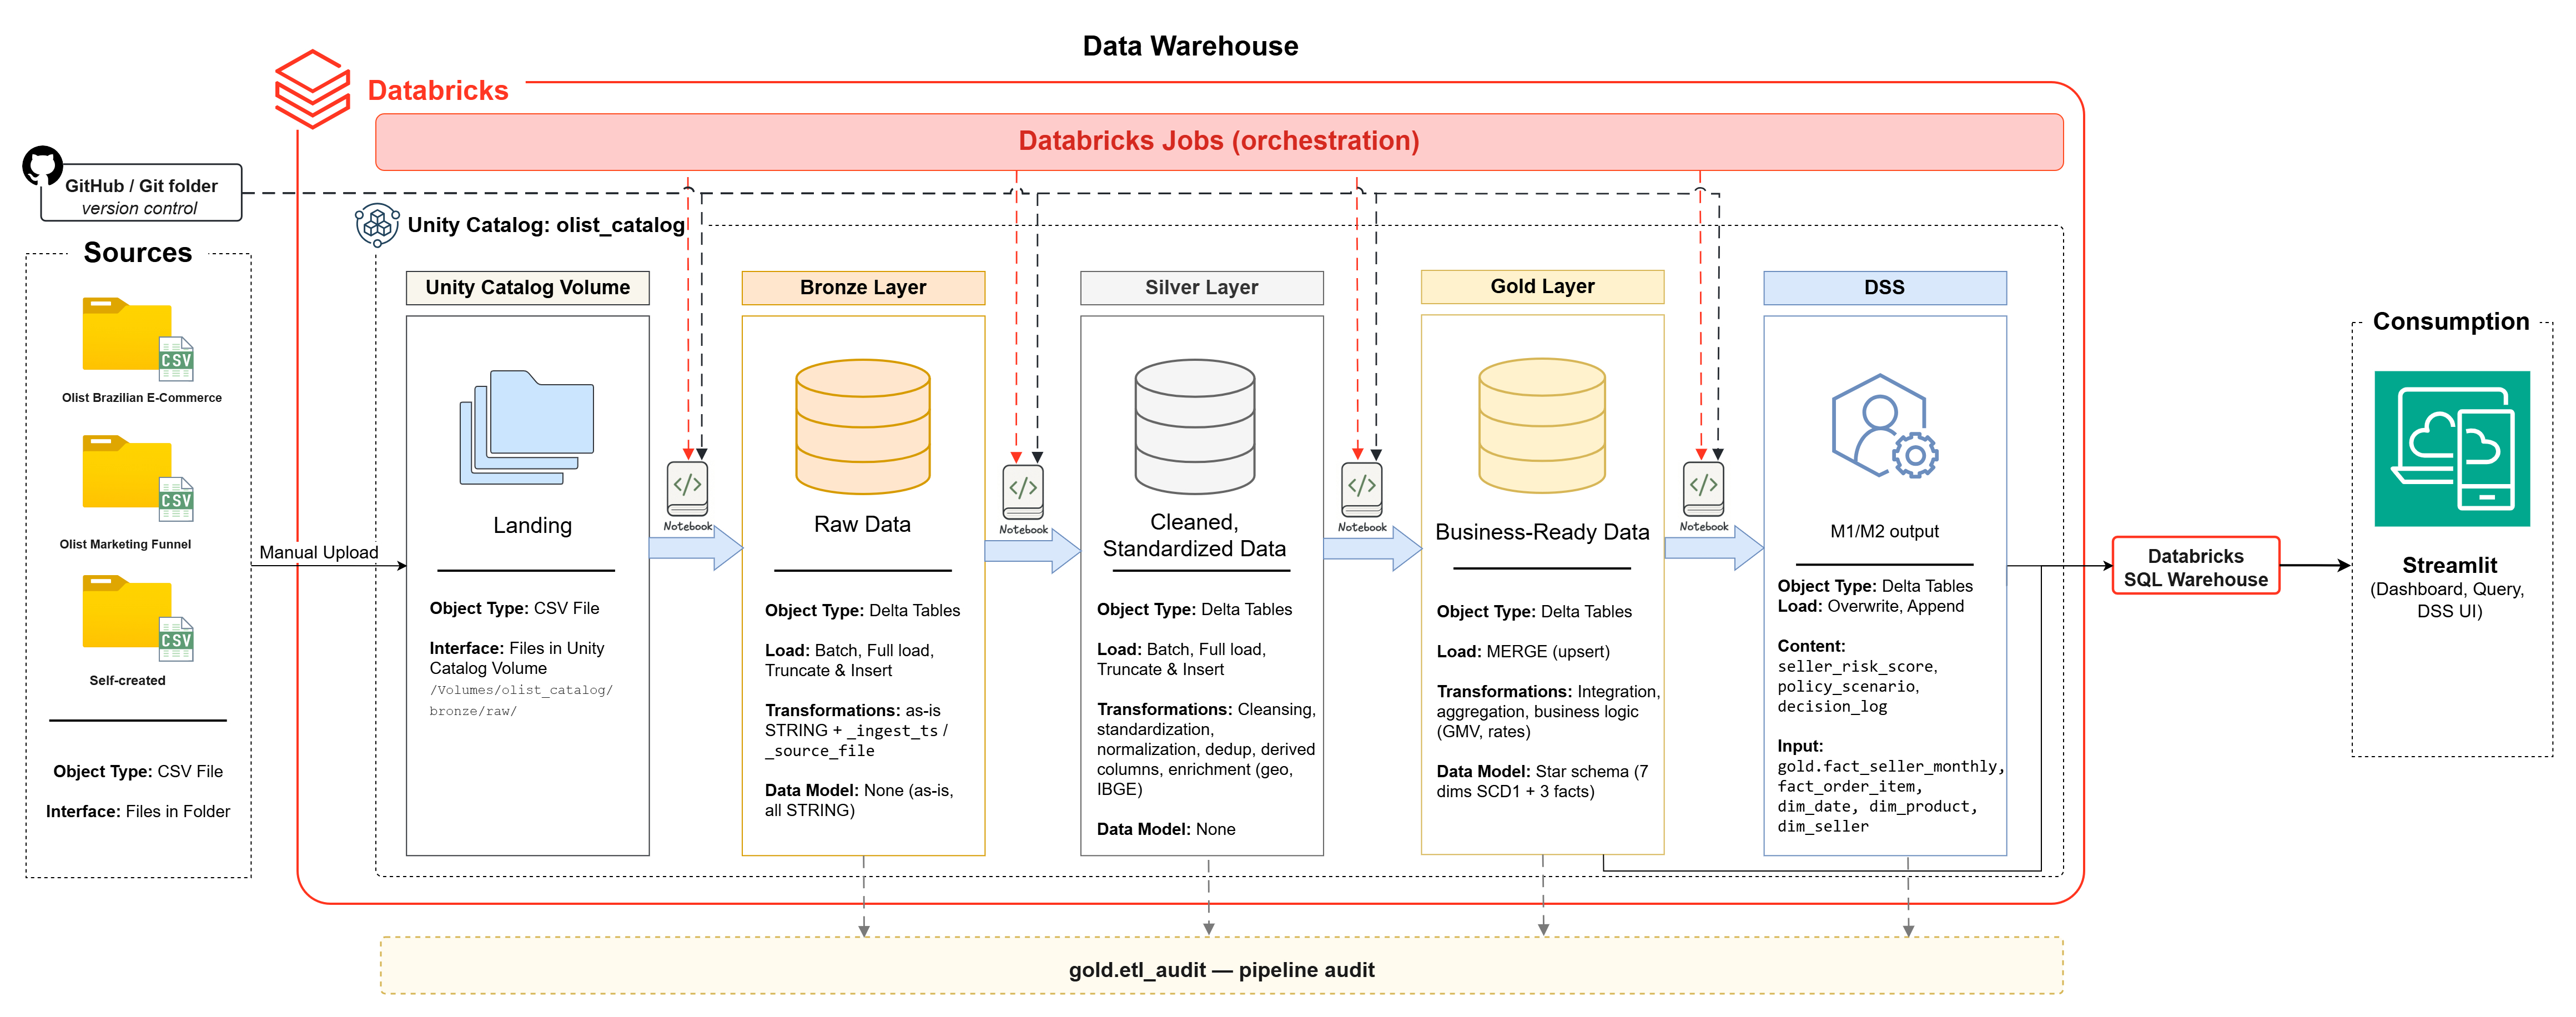
\includegraphics[width=0.92\textwidth]{images/high_level_architecture.drawio.png}%
}{%
  \fbox{\parbox{0.92\textwidth}{\centering\vspace{1.2cm}\textbf{[CẦN ẢNH]}~\texttt{images/high\_level\_architecture.drawio.png}\\Sơ đồ kiến trúc tổng thể hệ thống\vspace{1.2cm}}}%
}
\caption{Kiến trúc tổng thể hệ thống \texttt{olist-dw-dss}}
\label{fig:high_level_arch}
\end{figure}

\begin{table}[htbp]
\centering
\footnotesize
\setlength{\tabcolsep}{3pt}
\renewcommand{\arraystretch}{1.08}
\caption{Hợp đồng dữ liệu giữa các lớp kiến trúc (bản rút gọn)}
\label{tab:layer_contract}
\begin{tabularx}{\textwidth}{@{}>{\raggedright\arraybackslash}p{1.45cm}*{4}{>{\raggedright\arraybackslash}X}@{}}
\toprule
\textbf{Lớp} & \textbf{Đọc từ} & \textbf{Ghi vào} & \textbf{Cơ chế nạp} & \textbf{Ràng buộc chính} \\
\midrule
Volume & Tệp nguồn đã kiểm & CSV \texttt{olist/}, \texttt{funnel/}, \texttt{ref/} & Upload tay. Không phải bước của Job & Không sửa nội dung file. \\
\addlinespace
Bronze & Volume & 12 bảng Delta \texttt{bronze.*} & Full load, overwrite & Mọi cột nghiệp vụ \texttt{STRING}, giữ nguyên; thêm \texttt{\_ingest\_ts} và \texttt{\_source\_file}. Không join, không cast nghiệp vụ. \\
\addlinespace
Silver & Bronze & Bảng Delta đã chuẩn hóa & Full load, overwrite & Cast, chuẩn hóa, khử trùng trong file. Không chọn bản giữa hai lần nạp. \\
\addlinespace
Gold & Silver & 3 fact, 7 dimension, \texttt{etl\_audit} & \texttt{MERGE}: cập nhật khi khớp grain, thêm khi chưa có & Grain và khóa không trùng. Khóa ngoại không khớp trỏ member $-1$. Không xóa dòng nguồn đã mất. \\
\addlinespace
\texttt{dss} & Gold & \texttt{seller\_risk\_score}, \texttt{policy\_scenario}, \texttt{decision\_log} & Job DSS ghi đè hai bảng mô hình. Streamlit append \texttt{decision\_log} & Job ETL không ghi \texttt{dss}. Huấn luyện trên Gold. Streamlit không ghi hai bảng mô hình. \\
\bottomrule
\end{tabularx}
\end{table}

\subsection{Lựa chọn công nghệ}
\label{subsec:3_5}

Kho, lớp phân tích và hệ hỗ trợ quyết định cùng đọc một bản dữ liệu đã kiểm soát chất lượng. Bảng~\ref{tab:tech_choices} ghi từng lựa chọn và lý do.

\begin{table}[htbp]
\centering
\footnotesize
\setlength{\tabcolsep}{3pt}
\renewcommand{\arraystretch}{1.08}
\caption{Tổng hợp các lựa chọn công nghệ và lý do}
\label{tab:tech_choices}
\begin{tabularx}{\textwidth}{@{}>{\raggedright\arraybackslash}p{2.3cm}>{\raggedright\arraybackslash}X>{\raggedright\arraybackslash}X@{}}
\toprule
\textbf{Hạng mục} & \textbf{Lựa chọn} & \textbf{Lý do chọn} \\
\midrule
Nền tảng DW & Databricks Free Edition, Delta Lake, Unity Catalog & Một nền tảng cho lưu trữ, xử lý và phân quyền. Delta hỗ trợ \texttt{MERGE}, ràng buộc và \textit{time travel}. Môi trường miễn phí, serverless. \\
\addlinespace
OLAP & ROLAP trên Databricks SQL Warehouse & Truy vấn trực tiếp các bảng Gold bằng SQL, không phải bảo trì cube riêng. Quy mô dữ liệu vừa phải. \\
\addlinespace
Giao diện & Streamlit & Một ứng dụng cho KPI, OLAP và DSS, có tương tác \textit{what-if} và ghi lại quyết định. Power BI để hướng phát triển. \\
\addlinespace
Điều phối & Hai Databricks Job, tách ETL và DSS & Tách vòng đời nạp kho khỏi vòng đời mô hình. Chạy lại DSS không phải nạp lại kho. \\
\addlinespace
DSS & Huấn luyện và đọc từ tầng Gold & Dùng chung định nghĩa KPI đã kiểm soát chất lượng với lớp phân tích. Kết quả ghi vào schema \texttt{dss}. \\
\bottomrule
\end{tabularx}
\end{table}

%%%%%%%%%%%%%%%%%%%%%%%%%%%%%%%%%
% CHƯƠNG 4
%%%%%%%%%%%%%%%%%%%%%%%%%%%%%%%%%
\section{Thiết kế kho dữ liệu, ETL và chất lượng dữ liệu}
\label{sec:ch4}

Chương này trình bày thiết kế tầng Gold theo phương pháp mô hình hóa đa chiều của Kimball~\cite{bib:kimball2013}, quy trình ETL trên kiến trúc Medallion~\cite{bib:databricks} và cơ chế kiểm soát chất lượng dữ liệu. Tầng Gold gồm ba bảng fact, bảy bảng dimension và bảng nhật ký nạp \texttt{gold.etl\_audit}, tất cả là bảng Delta trong catalog \texttt{olist\_catalog}. Mục~\ref{subsec:4_1} và~\ref{subsec:4_2} mô tả mô hình dữ liệu, Mục~\ref{subsec:4_3} định nghĩa các KPI, Mục~\ref{subsec:4_4} và~\ref{subsec:4_5} trình bày đường ống nạp và các lớp kiểm soát.

\subsection{Fact constellation và grain}
\label{subsec:4_1}

Tầng Gold được tổ chức thành một \textit{fact constellation}: ba bảng fact dùng chung các \textit{conformed dimension}, như trên Hình~\ref{fig:erd_gold}. Nhóm tách thành ba fact vì các câu hỏi Q1--Q10 nằm ở ba mức chi tiết khác nhau. Bàn giao trễ (Q1, Q3, Q5) là sự kiện của từng dòng hàng, vì hạn bàn giao \texttt{shipping\_limit\_date} gắn với dòng hàng và mỗi dòng hàng thuộc đúng một người bán. Giao trễ tới khách và điểm review (Q2, Q4) là thuộc tính của cả đơn, vì nguồn chỉ có một mốc giao khách và sau làm sạch chỉ còn một review cho mỗi đơn. Hiệu suất người bán theo tháng (Q6--Q9) và đầu vào của mô hình M1 lại cần một ảnh định kỳ theo người bán và tháng. Nếu dồn cả ba vào một bảng, các measure cấp đơn sẽ bị lặp trên từng dòng hàng và bị cộng trùng khi tổng hợp~\cite{bib:kimball2013}.

\begin{figure}[htbp]
\centering
\IfFileExists{images/fig_4_1_erd.png}{%
  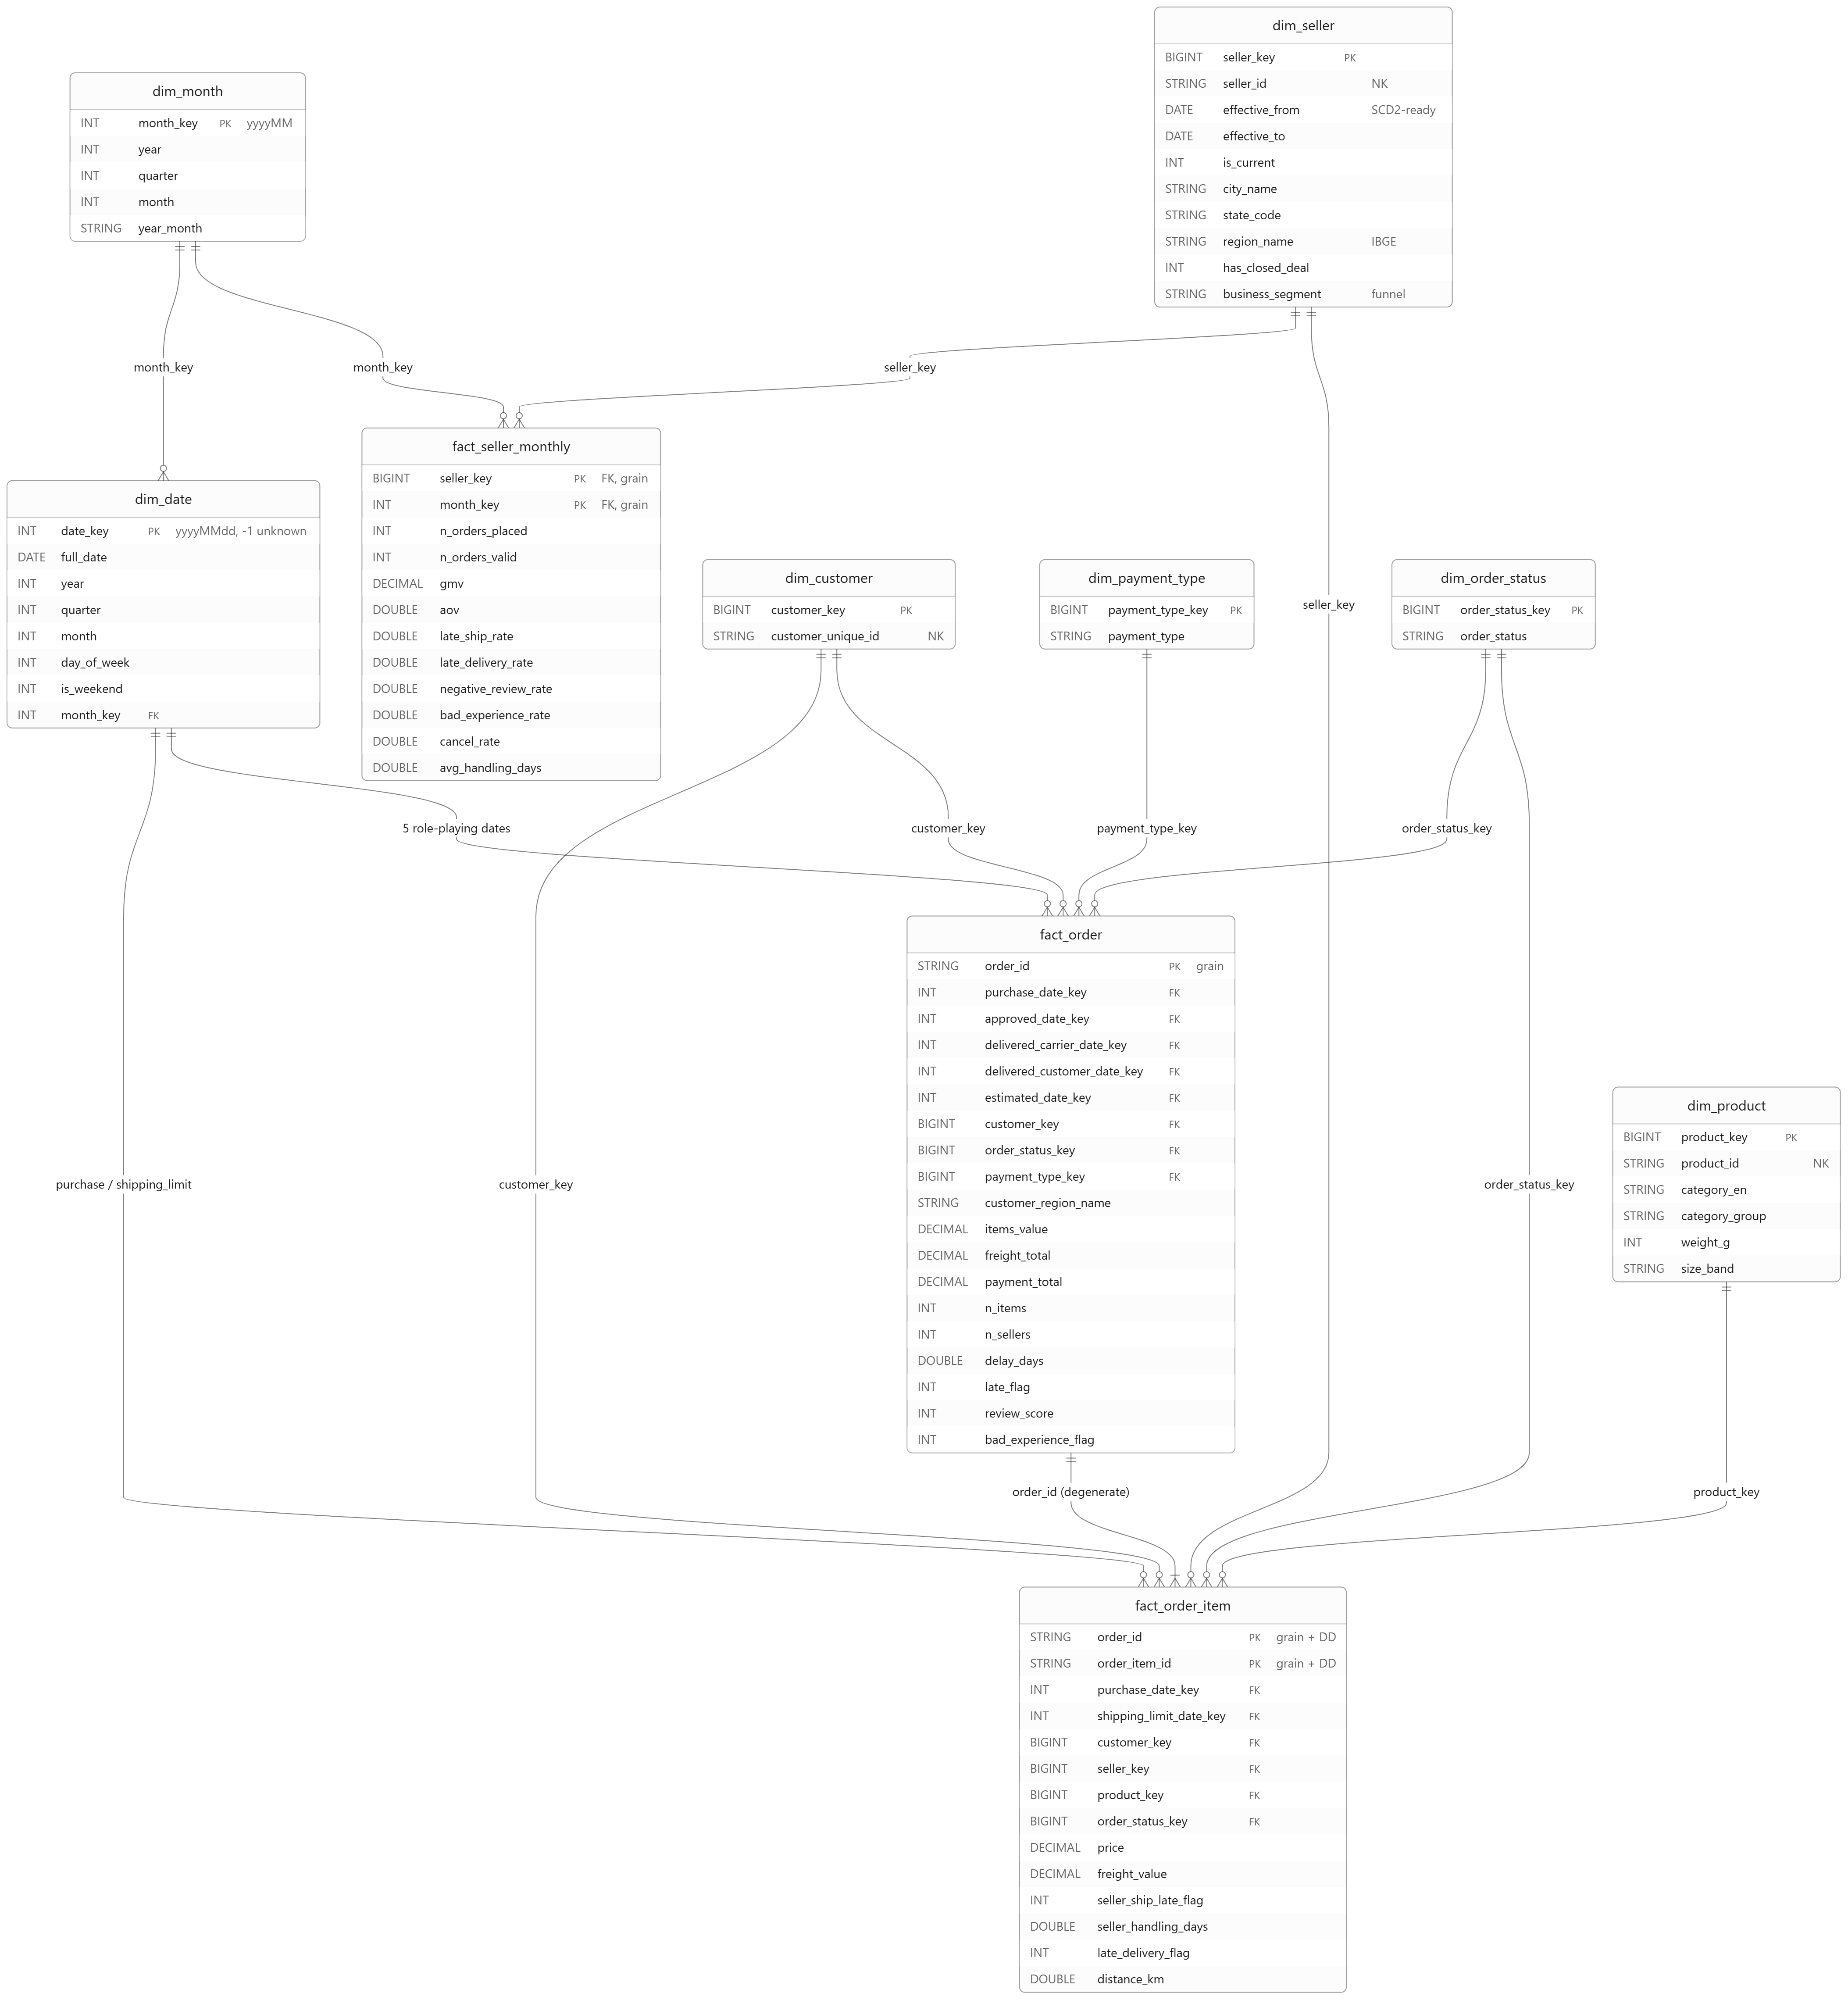
\includegraphics[width=\textwidth,height=0.78\textheight,keepaspectratio]{images/fig_4_1_erd.png}%
}{%
  \fbox{\parbox{0.92\textwidth}{\centering\vspace{1.2cm}\textbf{[CẦN ẢNH]}~\texttt{images/fig\_4\_1\_erd.png}\\Sơ đồ thực thể kết hợp (ERD) lược đồ sao/chòm sao Gold\vspace{1.2cm}}}%
}
\caption{Sơ đồ ERD mô hình đa chiều tầng Gold (rút gọn cột; danh sách cột đầy đủ ở Phụ lục PL.1)}
\label{fig:erd_gold}
\end{figure}

Bảng~\ref{tab:fact_tables} tóm tắt loại và grain của từng fact. \texttt{fact\_order\_item} là \textit{transaction fact}: mỗi dòng là một dòng hàng, khớp 112.650 dòng của tệp \texttt{order\_items}. Measure chính là \texttt{price} và \texttt{freight\_value} (cộng được), cờ bàn giao trễ \texttt{seller\_ship\_late\_flag}, thời gian xử lý \texttt{seller\_handling\_days} và khoảng cách \texttt{distance\_km} tính bằng công thức haversine giữa tọa độ người bán và tọa độ khách. \texttt{fact\_order} là \textit{accumulating snapshot}: mỗi đơn một dòng, mang năm mốc mua, duyệt, bàn giao vận chuyển, giao khách và hẹn giao, cùng các measure cấp đơn như \texttt{items\_value}, \texttt{payment\_total}, \texttt{n\_sellers}, \texttt{delay\_days}, \texttt{late\_flag}, \texttt{review\_score} và \texttt{bad\_experience\_flag}. Bảng có 99.441 dòng, bằng số đơn nguồn; 775 đơn không có dòng hàng vẫn được giữ với giá trị hàng bằng 0. Địa chỉ khách (vùng, bang, thành phố) đặt trên \texttt{fact\_order} chứ không trên \texttt{dim\_customer}, vì địa chỉ đi theo từng đơn (\texttt{customer\_id}), còn \texttt{dim\_customer} gom theo người (\texttt{customer\_unique\_id}). \texttt{fact\_seller\_monthly} là \textit{periodic snapshot}: mỗi dòng là một người bán trong một tháng mua có ít nhất một dòng hàng. Bảng không sinh dòng 0 cho tháng người bán không bán, và vẫn giữ sáu tháng thưa nếu tháng đó có đơn.

\begin{table}[htbp]
\centering
\footnotesize
\caption{Danh sách các bảng fact, loại fact và grain}
\label{tab:fact_tables}
\begin{tabularx}{\textwidth}{@{}>{\raggedright\arraybackslash}p{3.2cm}>{\raggedright\arraybackslash}p{3.0cm}>{\raggedright\arraybackslash}X@{}}
\toprule
\textbf{Bảng fact} & \textbf{Loại fact} & \textbf{Grain (mức chi tiết)} \\
\midrule
\texttt{fact\_order\_item} & Transaction & Một dòng là một mặt hàng trong đơn, khóa (\texttt{order\_id}, \texttt{order\_item\_id}) \\
\addlinespace
\texttt{fact\_order} & Accumulating snapshot & Một dòng là một đơn hàng (\texttt{order\_id}), theo dõi 5 mốc: mua, duyệt, bàn giao vận chuyển, giao khách, dự kiến giao \\
\addlinespace
\texttt{fact\_seller\_monthly} & Periodic snapshot & Một dòng là một người bán trong một tháng mua có ít nhất một mặt hàng (\texttt{seller\_key}, \texttt{month\_key}) \\
\bottomrule
\end{tabularx}
\end{table}

Bus matrix ở Bảng~\ref{tab:bus_matrix} cho biết fact nào dùng dimension nào. \texttt{dim\_date} là \textit{role-playing dimension}: một bảng vật lý được \texttt{fact\_order\_item} tham chiếu hai lần (ngày mua, hạn bàn giao) và \texttt{fact\_order} tham chiếu năm lần. \texttt{dim\_seller} là conformed dimension nối \texttt{fact\_order\_item} với \texttt{fact\_seller\_monthly}, nên số liệu chi tiết và ảnh tháng của cùng một người bán đọc theo cùng một bộ thuộc tính. \texttt{dim\_month} là dimension rút gọn từ \texttt{dim\_date}; \texttt{fact\_order\_item} lấy tháng qua \texttt{dim\_date.month\_key}. Hai fact cấp dòng hàng và cấp đơn liên kết qua \texttt{order\_id}, một \textit{degenerate dimension} nằm ngay trên fact. Gold không khai báo khóa ngoại giữa hai fact; câu hỏi cần cả hai mức, như Q4, dùng \textit{drill-across}: lọc vùng khách và quý trên \texttt{fact\_order}, nối \texttt{fact\_order\_item} để lấy nhóm kích thước hàng và người bán, rồi tính tỷ lệ trên tập đơn phân biệt.

\begin{table}[htbp]
\centering
\footnotesize
\caption{Bus matrix giữa các bảng fact và dimension}
\label{tab:bus_matrix}
\begin{tabularx}{\textwidth}{Xccccccc}
\toprule
\textbf{Fact} & \textbf{date} & \textbf{month} & \textbf{customer} & \textbf{seller} & \textbf{product} & \textbf{status} & \textbf{payment} \\
\midrule
\texttt{fact\_order\_item}     & \checkmark\,(2) & -- & \checkmark & \checkmark & \checkmark & \checkmark & -- \\
\texttt{fact\_order}           & \checkmark\,(5) & -- & \checkmark & -- & -- & \checkmark & \checkmark \\
\texttt{fact\_seller\_monthly} & -- & \checkmark & -- & \checkmark & -- & -- & -- \\
\bottomrule
\end{tabularx}

\vspace{2pt}
{\scriptsize Số trong ngoặc là số vai trò của \texttt{dim\_date} trên fact đó.}
\end{table}

Grain quyết định measure nào được cộng. \texttt{price}, \texttt{gmv}, \texttt{n\_items\_placed} và \texttt{n\_items\_valid} cộng được qua người bán, vì mỗi dòng hàng thuộc đúng một người bán. Ngược lại, \texttt{n\_orders\_placed} và \texttt{n\_orders\_valid} trên \texttt{fact\_seller\_monthly} không cộng được qua người bán. Trong 98.666 đơn có dòng hàng, 1.278 đơn thuộc hơn một người bán; mỗi đơn như vậy được đếm một lần cho từng người bán của nó, nên cộng ngang các dòng người bán sẽ đếm đơn nhiều lần. Các bộ đếm theo đơn khác (giao trễ, review, trải nghiệm xấu, hủy) có cùng tính chất. Vì vậy số đơn toàn sàn luôn đọc từ \texttt{fact\_order}, còn \texttt{fact\_seller\_monthly} chỉ dùng cho phân tích theo từng người bán. Các đơn nhiều người bán không bị xóa; chúng vẫn nằm trong fact, trong GMV và trong cờ giao trễ, chỉ bị loại khỏi measure review của người bán (Mục~\ref{subsec:4_3}).

\subsection{Dimension, khóa và SCD}
\label{subsec:4_2}

Gold có bảy dimension, tóm tắt ở Bảng~\ref{tab:dim_hierarchies}; danh sách cột đầy đủ nằm ở Phụ lục~\hyperref[pl:1]{PL.1}. \texttt{dim\_date} sinh mọi ngày từ ngày nhỏ nhất đến ngày lớn nhất trong các mốc thời gian đã parse ở Silver, kể cả những ngày không có đơn, để chuỗi thời gian không bị đứt. Bảng không dùng lịch ngày lễ vì không có nguồn công khai phù hợp cho giai đoạn 2016--2018. \texttt{dim\_month} giữ một dòng cho mỗi tháng có trong \texttt{dim\_date}, phục vụ grain tháng của \texttt{fact\_seller\_monthly}.

\begin{table}[htbp]
\centering
\footnotesize
\setlength{\tabcolsep}{3pt}
\renewcommand{\arraystretch}{1.08}
\caption{Các dimension và hệ thống phân cấp (hierarchy)}
\label{tab:dim_hierarchies}
\begin{tabularx}{\textwidth}{@{}>{\raggedright\arraybackslash}p{2.7cm}>{\raggedright\arraybackslash}X>{\raggedright\arraybackslash}X@{}}
\toprule
\textbf{Dimension} & \textbf{SCD / Đặc điểm} & \textbf{Hierarchy / Vai trò} \\
\midrule
\texttt{dim\_date} & Khóa \texttt{date\_key} = \texttt{yyyyMMdd}. Role-playing: 2 vai trên \texttt{fact\_order\_item}, 5 vai trên \texttt{fact\_order}. Có \texttt{day\_of\_week}, \texttt{is\_weekend} & Năm $\to$ Quý $\to$ Tháng $\to$ Ngày \\
\addlinespace
\texttt{dim\_month} & Khóa \texttt{month\_key} = \texttt{yyyyMM}. Dimension rút gọn từ \texttt{dim\_date} & Năm $\to$ Quý $\to$ Tháng; grain của \texttt{fact\_seller\_monthly} \\
\addlinespace
\texttt{dim\_customer} & SCD1. Một dòng mỗi \texttt{customer\_unique\_id}; không giữ địa chỉ & Khách hàng; địa lý khách nằm trên \texttt{fact\_order}: Vùng $\to$ Bang $\to$ Thành phố \\
\addlinespace
\texttt{dim\_seller} & SCD1, thiết kế sẵn cho SCD2: \texttt{effective\_from}, \texttt{effective\_to}, \texttt{is\_current}. Thuộc tính funnel: \texttt{has\_closed\_deal}, \texttt{business\_segment}, \texttt{lead\_type}, \texttt{won\_date} & Vùng (IBGE) $\to$ Bang $\to$ Thành phố; Phân khúc $\to$ Người bán \\
\addlinespace
\texttt{dim\_product} & SCD1. Thiếu danh mục vẫn là thành viên dương, nhãn \texttt{'Unknown'}. Có \texttt{size\_band} (small, medium, bulky) & Nhóm danh mục (8 nhóm) $\to$ Danh mục $\to$ Sản phẩm \\
\addlinespace
\texttt{dim\_order\_status} & SCD1. Giữ đúng chuỗi trạng thái nguồn & Lọc đơn hợp lệ, đơn hủy \\
\addlinespace
\texttt{dim\_payment\_type} & SCD1. \texttt{not\_defined} và rỗng trỏ về thành viên $-1$ & Phương thức thanh toán chính của đơn \\
\bottomrule
\end{tabularx}
\end{table}

\textbf{Khóa.} Mọi dimension dùng \textit{surrogate key}; natural key như \texttt{seller\_id}, \texttt{product\_id} hay \texttt{customer\_\allowbreak{}unique\_\allowbreak{}id} chỉ là thuộc tính. Hai dimension thời gian dùng khóa số có nghĩa (\texttt{yyyyMMdd}, \texttt{yyyyMM}) để dễ lọc và dễ đọc. Năm dimension còn lại dùng khóa \texttt{BIGINT} cấp theo cách tất định: natural key đã có giữ nguyên khóa cũ; natural key mới nhận khóa bằng giá trị lớn nhất hiện có cộng số thứ tự \texttt{row\_number()} khi sắp xếp tăng dần theo natural key. Nhờ vậy, chạy lại trên cùng dữ liệu luôn sinh cùng một khóa, và khóa không đổi giữa các lần nạp nên fact không phải nạp lại khi dimension có thêm thành viên.

\textbf{Thành viên Unknown.} Trước khi nạp fact, mỗi dimension được \texttt{MERGE} một dòng khóa $-1$. Thuộc tính chữ dùng để nhóm trên dòng này mang nhãn \texttt{'Unknown'}, natural key và thuộc tính số để null. Khi khóa ngoại của fact thiếu hoặc không khớp, ví dụ mốc thời gian null hay loại thanh toán không xác định, dòng fact vẫn được giữ và trỏ về $-1$ thay vì bị loại. Số lần trỏ về $-1$ được ghi vào cột \texttt{rows\_unknown\_fk} của \texttt{gold.etl\_audit}. Cách này giữ đủ tổng tiền và tổng số đơn, đồng thời bảo đảm mọi phép \texttt{JOIN} fact--dimension đều khớp.

\textbf{SCD.} Mọi dimension dùng \textit{SCD Type 1}, vì cả Olist lẫn Marketing Funnel chỉ cung cấp trạng thái hiện tại, không có lịch sử thay đổi thuộc tính. \texttt{dim\_seller} được thiết kế sẵn cho Type 2: bảng có \texttt{effective\_from} (mốc quy ước 1900-01-01), \texttt{effective\_to} (null) và \texttt{is\_current} = 1 trên mỗi người bán, còn fact chỉ trỏ \texttt{seller\_key}. Khi có nguồn lịch sử, ví dụ người bán đổi bang kho hàng, chỉ cần thêm phiên bản mới và tra khóa theo ngày mua; cấu trúc fact không đổi. Trên Gold hiện có 3.095 người bán và 96.096 khách hàng, không tính dòng $-1$, khớp số \texttt{seller\_id} và số \texttt{customer\_unique\_id} phân biệt của nguồn.

\textbf{Phân cấp.} Ngoài phân cấp thời gian, Gold có ba phân cấp phục vụ roll-up và drill-down. Địa lý người bán đi từ vùng IBGE xuống bang và thành phố đã chuẩn hóa. Sản phẩm đi từ nhóm danh mục xuống danh mục và sản phẩm; tám nhóm danh mục do nhóm định nghĩa từ 73 tên danh mục gốc, danh mục không thuộc bảy nhóm chính rơi vào nhóm dịch vụ và khác. \texttt{size\_band} xếp sản phẩm thành \textit{bulky} khi nặng từ 10.000\,g hoặc thể tích từ 30.000\,cm$^3$, \textit{medium} khi từ 2.000\,g hoặc 8.000\,cm$^3$, còn lại là \textit{small}; đây là ngưỡng quy ước, phục vụ phép dice của Q4.

\subsection{Định nghĩa measure và KPI}
\label{subsec:4_3}

Các measure tuân theo ba quy ước. Tiền dùng kiểu \texttt{DECIMAL(18,2)}. Cờ dùng \texttt{INT} 0/1 và để null khi không tính được, để đơn thiếu dữ liệu ra khỏi cả tử lẫn mẫu. Tỷ lệ và AOV là measure không cộng được: \texttt{fact\_seller\_monthly} lưu cả tử số, mẫu số và tỷ lệ, nhưng cột tỷ lệ chỉ để đọc nhanh. Mọi phép roll-up phải tính $\sum \text{tử} / \sum \text{mẫu}$ thay vì lấy trung bình các tỷ lệ con; lấy trung bình sẽ cho một người bán có 5 đơn cùng trọng số với người bán có 500 đơn. Bảng~\ref{tab:kpi_definitions} định nghĩa tám KPI cấp người bán--tháng.

\begin{table}[htbp]
\centering
\footnotesize
\setlength{\tabcolsep}{3pt}
\renewcommand{\arraystretch}{1.08}
\caption{Định nghĩa KPI, công thức, mẫu tính và quy tắc loại trừ}
\label{tab:kpi_definitions}
\begin{tabularx}{\textwidth}{@{}>{\raggedright\arraybackslash}p{2.35cm}>{\raggedright\arraybackslash}p{3.6cm}>{\raggedright\arraybackslash}p{3.6cm}>{\raggedright\arraybackslash}X@{}}
\toprule
\textbf{KPI} & \textbf{Công thức} & \textbf{Mẫu (denominator)} & \textbf{Loại trừ / ghi chú} \\
\midrule
GMV & $\sum$ \texttt{price} của dòng hàng trong tháng mua & Không có (measure cộng được) & Loại đơn \texttt{canceled}, \texttt{unavailable}; không cộng cước \texttt{freight\_\allowbreak{}value} \\
\addlinespace
AOV & \texttt{gmv} / \texttt{n\_\allowbreak{}orders\_\allowbreak{}valid} & Số đơn hợp lệ phân biệt của người bán & Null khi mẫu bằng 0; tính lại từ GMV và số đơn, không lấy trung bình \\
\addlinespace
Tỷ lệ bàn giao trễ (\texttt{late\_\allowbreak{}ship\_\allowbreak{}rate}) & Số dòng hàng có \texttt{seller\_\allowbreak{}ship\_\allowbreak{}late\_\allowbreak{}flag} = 1 & Số dòng hàng có cờ khác null & Cờ null khi đơn hủy, thiếu hạn bàn giao hoặc mốc bàn giao bị đảo; chưa bàn giao mà quá hạn trước ngày chốt thì tính trễ \\
\addlinespace
Tỷ lệ giao trễ (\texttt{late\_\allowbreak{}delivery\_\allowbreak{}rate}) & Số đơn có \texttt{late\_\allowbreak{}flag} = 1 (ngày giao sau ngày hẹn) & Số đơn phân biệt có cờ khác null & Đơn hủy và đơn thiếu ngày giao hoặc ngày hẹn nằm ngoài mẫu \\
\addlinespace
Tỷ lệ review xấu (\texttt{negative\_\allowbreak{}review\_\allowbreak{}rate}) & Số đơn có điểm $\le 2$ & \texttt{COUNT(DISTINCT order\_\allowbreak{}id)} có điểm, một người bán, review không dùng chung khác người bán & Loại đơn nhiều người bán và \texttt{cross\_\allowbreak{}seller}; KPI toàn sàn giữ hai nhóm này \\
\addlinespace
Tỷ lệ trải nghiệm xấu (\texttt{bad\_\allowbreak{}experience\_\allowbreak{}rate}) & Số đơn có review xấu quy cho người bán \textbf{hoặc} giao trễ & Số đơn phân biệt còn lại sau hai nhánh & Nhánh review theo luật dòng trên; nhánh giao trễ giữ cả đơn nhiều người bán; hủy không tính \\
\addlinespace
Tỷ lệ hủy (\texttt{cancel\_\allowbreak{}rate}) & Số đơn \texttt{canceled} hoặc \texttt{unavailable} & \texttt{n\_\allowbreak{}orders\_\allowbreak{}placed} (mọi trạng thái) & Đơn hủy chỉ vào chỉ số này, không vào cờ trễ \\
\addlinespace
Thời gian xử lý (\texttt{avg\_\allowbreak{}handling\_\allowbreak{}days}) & $\sum$ (bàn giao $-$ duyệt), tính bằng ngày & Số dòng hàng có đủ hai mốc & Mốc bị đảo đã thành null nên không vào trung bình \\
\bottomrule
\end{tabularx}
\end{table}

Bàn giao trễ và giao trễ là hai chỉ số khác nhau và không được dùng thay nhau. Bàn giao trễ đo lỗi của người bán: so mốc bàn giao cho đơn vị vận chuyển với hạn \texttt{shipping\_limit\_date}, theo timestamp, ở cấp dòng hàng. Giao trễ đo kết quả của cả chuỗi giao vận: so ngày khách nhận với ngày hẹn, theo ngày lịch, ở cấp đơn. Một đơn có thể được người bán bàn giao đúng hạn nhưng vẫn tới khách trễ do vận chuyển, và ngược lại. Khi mốc bàn giao thật sự thiếu, cờ chỉ bật nếu hạn bàn giao đã qua trước ngày chốt dữ liệu 2018-10-17; hạn từ ngày đó trở đi được coi là chưa đến hạn. Vì nguồn chỉ có một mốc bàn giao cho cả đơn, 1.278 đơn nhiều người bán dùng chung mốc này, nên cờ trên các đơn đó kém tin cậy hơn; đây là hạn chế của dữ liệu và được nêu lại ở Chương~\ref{sec:ch6}.

Review cần một luật quy trách nhiệm riêng. Profiling cho thấy 789 \texttt{review\_id} gắn với nhiều đơn (Bảng~\ref{tab:profiling_issues}), và Olist không công bố nguyên nhân. Sau khi giữ review mới nhất cho mỗi đơn, mỗi đơn được gắn \texttt{shared\_review\_type}: \texttt{none} khi review chỉ thuộc một đơn, \texttt{same\_seller} khi các đơn dùng chung review cùng một người bán, và \texttt{cross\_seller} khi chúng thuộc nhiều người bán. Measure review của người bán chỉ giữ đơn một người bán với loại \texttt{none} hoặc \texttt{same\_seller}, vì không thể biết điểm của đơn \texttt{cross\_seller} hay đơn nhiều người bán thuộc về ai. KPI toàn sàn vẫn giữ mọi điểm. Review bị loại khỏi measure người bán không tắt nhánh giao trễ, nên người bán không thoát khỏi chỉ số trải nghiệm xấu chỉ vì review bị loại. Mẫu số của mọi tỷ lệ review là \texttt{COUNT(DISTINCT order\_id)}, không đếm \texttt{review\_id}.

Trên toàn bộ Gold, không áp bộ lọc, tỷ lệ bàn giao trễ là 11.132/110.550 dòng hàng (10,07\%), tỷ lệ review xấu theo người bán là 13.141/95.974 đơn (13,69\%), tỷ lệ hủy là 467/98.666 đơn (0,47\%), tỷ lệ đơn trải nghiệm xấu toàn sàn là 16.444/98.079 đơn (16,77\%), và AOV là 13.494.400,74/98.199 = R\$~137,42. Review của 1.943 đơn bị loại khỏi measure người bán theo luật trên.

\subsection{Pipeline ETL}
\label{subsec:4_4}

Đường ống nạp kho là Job \texttt{olist\_etl} chạy trên compute serverless của Databricks, gồm sáu task nối tiếp: \texttt{setup}, \texttt{bronze}, \texttt{silver}, \texttt{gold\_dims}, \texttt{gold\_facts} và \texttt{fact\_seller\_monthly} (Hình~\ref{fig:etl_dag}). Mọi task nhận chung tham số catalog, schema, đường dẫn Volume, ngày chốt và \texttt{run\_id} bằng mã lần chạy của Job, nên các dòng nhật ký của một lần nạp được nhóm theo cùng \texttt{run\_id}. Job dừng ở Gold; mô hình DSS chạy trong một Job riêng (Chương~\ref{sec:ch5}). Ánh xạ cột chi tiết từ CSV qua Bronze, Silver đến Gold nằm ở Phụ lục~\hyperref[pl:2]{PL.2}.

\begin{figure}[htbp]
\centering
\IfFileExists{images/fig_4_2_etl_dag.png}{%
  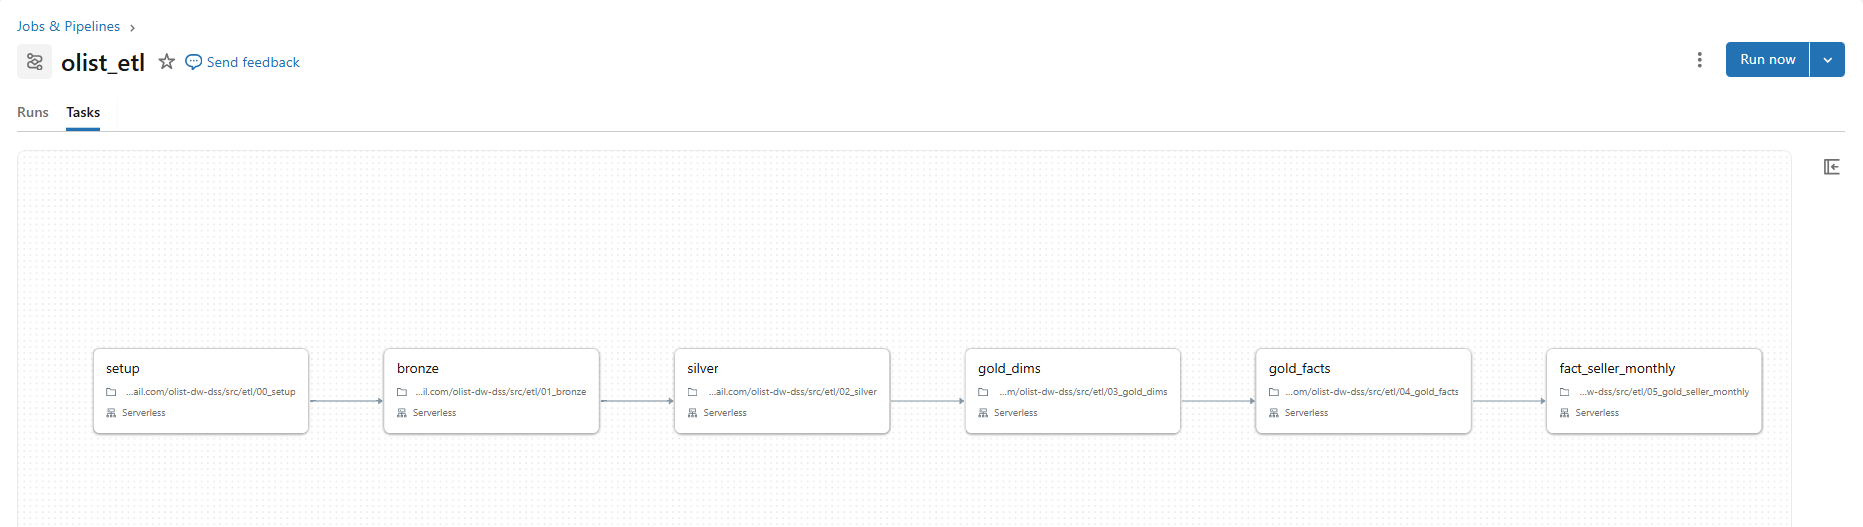
\includegraphics[width=\textwidth]{images/fig_4_2_etl_dag.png}%
}{%
  \fbox{\parbox{0.90\textwidth}{\centering\vspace{1.0cm}\textbf{[CẦN ẢNH]}~\texttt{images/fig\_4\_2\_etl\_dag.png}\\Ảnh chụp DAG Job \texttt{olist\_etl} (6 task) trên Databricks\vspace{1.0cm}}}%
}
\caption{Đồ thị thực thi (DAG) của Job \texttt{olist\_etl} trên Databricks}
\label{fig:etl_dag}
\end{figure}

\textbf{Setup và Bronze.} Task \texttt{setup} tạo bốn schema \texttt{bronze}, \texttt{silver}, \texttt{gold}, \texttt{dss} và bảng \texttt{gold.etl\_audit} nếu chưa có, rồi kiểm tra Volume đã có đủ ba thư mục \texttt{olist/}, \texttt{funnel/}, \texttt{ref/}; task không tạo lại hay xóa Volume. Task \texttt{bronze} đọc 12 tệp CSV với dòng tiêu đề và không suy kiểu. Mọi cột nghiệp vụ được giữ ở kiểu \texttt{STRING}, đúng như tệp: không \texttt{trim}, không ép số, giữ số 0 đầu của mã zip. Chỉ tên cột được chuẩn hóa (bỏ BOM và dấu nháy thừa). Mỗi bảng có thêm \texttt{\_ingest\_ts} (thời điểm đọc) và \texttt{\_source\_file} (đường dẫn tệp) để truy vết nguồn gốc. Bronze nạp toàn phần và ghi đè, nên số dòng luôn bằng số dòng tệp hiện tại; notebook in số dòng đã nạp để đối chiếu với số đã đo khi kiểm kê.

\textbf{Silver.} Task \texttt{silver} ép kiểu và làm sạch vào các bảng có DDL với ràng buộc \texttt{NOT NULL}; mỗi lần nạp ghi đè dữ liệu nhưng giữ nguyên schema. Mã và zip được \texttt{trim}, chuỗi rỗng thành null. Timestamp được parse theo mẫu \texttt{yyyy-MM-dd HH:mm:ss}, lỗi parse thành null. Tiền âm bị đặt null nhưng dòng vẫn được giữ và được in trong kiểm tra chất lượng. Các luật xử lý vấn đề đã nêu ở Bảng~\ref{tab:profiling_issues} được cài như sau:
\begin{itemize}
  \item \textit{Thành phố và vùng}: \texttt{city\_\allowbreak{}norm} = chữ thường, bỏ dấu tiếng Bồ Đào Nha, \texttt{trim}, dùng chung cho khách, người bán và geolocation; mã bang viết hoa rồi nối bảng IBGE để lấy vùng.
  \item \textit{Geolocation}: bỏ điểm ngoài khung Brazil (vĩ độ $[-34, 6]$, kinh độ $[-74, -28]$), lấy trung vị vĩ độ, kinh độ (\texttt{percentile\_\allowbreak{}approx} 0,5) và thành phố, bang phổ biến nhất cho mỗi tiền tố zip. Tọa độ của khách và người bán tra theo zip, nếu không có thì theo (thành phố, bang), nếu vẫn không có thì để null; cột \texttt{geo\_\allowbreak{}match\_\allowbreak{}level} ghi mức khớp. Không điền 0 để tránh khoảng cách giả.
  \item \textit{Review}: \texttt{silver.order\_\allowbreak{}reviews} giữ một dòng cho mỗi (\texttt{review\_\allowbreak{}id}, \texttt{order\_\allowbreak{}id}), ưu tiên bản có \texttt{review\_\allowbreak{}answer\_\allowbreak{}timestamp} mới nhất; \texttt{silver.order\_\allowbreak{}reviews\_\allowbreak{}dedup} giữ một review cho mỗi đơn theo cùng thứ tự và gắn \texttt{shared\_\allowbreak{}review\_\allowbreak{}type}.
  \item \textit{Mốc thời gian đảo}: khi một mốc đứng trước mốc lẽ ra phải có trước, cột chính thức bị đặt null, giá trị gốc giữ ở cột \texttt{raw\_\allowbreak{}*} và \texttt{ts\_\allowbreak{}inversion\_\allowbreak{}flag} = 1. Phép so sánh dùng cột \texttt{raw\_\allowbreak{}*} để một mốc bị xóa không kéo theo các mốc khác.
  \item \textit{Khóa trùng trong tệp}: giữ một dòng theo chuỗi ghép các cột nghiệp vụ lớn nhất theo thứ tự từ điển, để kết quả tất định khi chạy lại.
\end{itemize}

\textbf{Gold.} Task \texttt{gold\_dims} chèn thành viên $-1$ rồi \texttt{MERGE} bảy dimension theo natural key. Task \texttt{gold\_facts} tính các cờ cấp đơn một lần từ Silver, \texttt{MERGE} \texttt{fact\_order\_item} trước (cờ giao trễ được lặp xuống từng dòng hàng), rồi \texttt{MERGE} \texttt{fact\_order} với cùng giá trị cờ. Task cuối tổng hợp \texttt{fact\_seller\_monthly} từ hai fact đó. Mọi lệnh \texttt{MERGE} ở Gold chỉ có hai nhánh: cập nhật khi khớp grain và chèn khi chưa có (Đoạn mã~\ref{lst:gold_merge}). Không có nhánh xóa dòng vắng mặt ở nguồn, vì bộ dữ liệu là tập tĩnh; nhờ đó thành viên $-1$ và các khóa đã nạp không bị mất, và chạy lại cùng dữ liệu không nhân đôi dòng.

\renewcommand{\lstlistingname}{Đoạn mã}
\begin{lstlisting}[language=Python,caption={Hàm MERGE dùng chung cho các bảng fact, trích từ \texttt{src/etl/04\_gold\_facts.py}},label={lst:gold_merge}]
def merge_fact(table: str, frame: DataFrame, on_sql: str) -> None:
    align(frame, table).createOrReplaceTempView("fact_src")
    spark.sql(
        f"""
        MERGE INTO {table} t
        USING fact_src s
        ON {on_sql}
        WHEN MATCHED THEN UPDATE SET *
        WHEN NOT MATCHED THEN INSERT *
        """
    )

merge_fact(item_table, item_fact,
           "t.order_id = s.order_id AND t.order_item_id = s.order_item_id")
merge_fact(order_table, order_calc, "t.order_id = s.order_id")
\end{lstlisting}

Nhóm chọn nạp toàn phần cho Bronze và Silver, \texttt{MERGE} cho Gold. Với tập dữ liệu tĩnh, ghi đè toàn phần là cách đơn giản nhất để hai lớp đầu luôn khớp tệp nguồn, không cần watermark hay luật chọn bản ghi giữa các lần nạp. Ở Gold, \texttt{MERGE} theo grain giữ ổn định surrogate key và bảo đảm tính idempotent; Delta Lake thực hiện lệnh này trong một giao dịch ACID~\cite{bib:databricks}. Nạp tăng dần bằng Change Data Feed hoặc Auto Loader được để làm hướng phát triển (Mục~\ref{subsec:6_4}).

\subsection{Chất lượng dữ liệu và kiểm soát}
\label{subsec:4_5}

Chất lượng dữ liệu được kiểm soát ở ba lớp. Lớp thứ nhất là ràng buộc \texttt{CHECK} của Delta trên từng dòng fact; một dòng vi phạm làm lệnh ghi thất bại thay vì lặng lẽ đi vào kho. \texttt{chk\_foi\_money} yêu cầu \texttt{price} và \texttt{freight\_value} không âm; \texttt{chk\_foi\_flags} và \texttt{chk\_fo\_flags} giới hạn các cờ trong \{0, 1\} hoặc null; \texttt{chk\_fo\_amounts\_counts} yêu cầu tiền và bộ đếm của đơn không âm; \texttt{chk\_fo\_review} giới hạn điểm trong 1--5 và buộc \texttt{review\_score} cùng \texttt{shared\_review\_type} đồng thời null hoặc đồng thời có giá trị. Trên \texttt{fact\_seller\_monthly}, \texttt{chk\_fsm\_totals} kiểm số đơn hợp lệ không vượt số đơn đã đặt và AOV null khi không có đơn hợp lệ, \texttt{chk\_fsm\_num\_den} kiểm tử số không vượt mẫu số, \texttt{chk\_fsm\_rates} kiểm mọi tỷ lệ nằm trong $[0, 1]$. Cột grain và khóa ngoại khai báo \texttt{NOT NULL}.

Lớp thứ hai là bảng \texttt{gold.etl\_audit}, chỉ ghi thêm, mỗi bảng đích của mỗi lần chạy một dòng. Mười cột gồm \texttt{audit\_id}, \texttt{run\_id}, \texttt{layer}, \texttt{target\_table}, \texttt{source\_name}, \texttt{rows\_read}, \texttt{rows\_loaded}, \texttt{rows\_rejected} (dòng bị bỏ hẳn, không gồm khử trùng), \texttt{rows\_unknown\_fk} (số khóa ngoại trỏ $-1$, chỉ với fact) và \texttt{loaded\_at}. Bảng~\ref{tab:etl_audit} là kết quả của một lần chạy hoàn chỉnh.

\begin{table}[htbp]
\centering
\scriptsize
\setlength{\tabcolsep}{2pt}
\renewcommand{\arraystretch}{1.08}
\caption{Kết quả \texttt{gold.etl\_audit} của một lần chạy hoàn chỉnh}
\label{tab:etl_audit}
\begin{tabularx}{\textwidth}{@{}>{\raggedright\arraybackslash}p{2.9cm}rrrr>{\raggedright\arraybackslash}X@{}}
\toprule
\textbf{Bảng đích} & \textbf{rows\_read} & \textbf{rows\_loaded} & \textbf{rows\_rejected} & \textbf{unknown\_fk} & \textbf{Số đối chiếu đã đo} \\
\midrule
12 bảng \texttt{bronze.*} & \textbf{[CẦN SỐ]} & \textbf{[CẦN SỐ]} & \textbf{[CẦN SỐ]} & -- & Bằng số dòng tệp ở Bảng~\ref{tab:data_sources} \\
\addlinespace
\texttt{silver.orders} & \textbf{[CẦN SỐ]} & \textbf{[CẦN SỐ]} & \textbf{[CẦN SỐ]} & -- & 99.441 đơn trong tệp \\
\addlinespace
\texttt{silver.order\_\allowbreak{}reviews\_\allowbreak{}dedup} & \textbf{[CẦN SỐ]} & \textbf{[CẦN SỐ]} & \textbf{[CẦN SỐ]} & -- & Tệp 99.224 dòng; một review mỗi đơn \\
\addlinespace
\texttt{silver.geolocation\_zip} & \textbf{[CẦN SỐ]} & \textbf{[CẦN SỐ]} & \textbf{[CẦN SỐ]} & -- & 1.000.163 điểm; 31 điểm ngoài khung bị loại \\
\addlinespace
7 dimension Gold & \textbf{[CẦN SỐ]} & \textbf{[CẦN SỐ]} & \textbf{[CẦN SỐ]} & -- & \texttt{dim\_seller} 3.095; \texttt{dim\_customer} 96.096 (không tính $-1$) \\
\addlinespace
\texttt{fact\_order\_item} & \textbf{[CẦN SỐ]} & \textbf{[CẦN SỐ]} & \textbf{[CẦN SỐ]} & \textbf{[CẦN SỐ]} & 112.650 dòng hàng nguồn \\
\addlinespace
\texttt{fact\_order} & \textbf{[CẦN SỐ]} & \textbf{[CẦN SỐ]} & \textbf{[CẦN SỐ]} & \textbf{[CẦN SỐ]} & 99.441 dòng trên Gold \\
\addlinespace
\texttt{fact\_seller\_monthly} & \textbf{[CẦN SỐ]} & \textbf{[CẦN SỐ]} & \textbf{[CẦN SỐ]} & \textbf{[CẦN SỐ]} & \textbf{[CẦN SỐ]} cặp người bán--tháng \\
\bottomrule
\end{tabularx}
\end{table}

Lớp thứ ba là các kiểm tra in ra trong notebook. Kiểm tra đối soát xác nhận $\textit{rows\_read} = \textit{rows\_loaded} + \textit{rows\_dropped\_by\_dedup} + \textit{rows\_rejected}$ cho từng bảng trong cùng \texttt{run\_id}. Kiểm tra grain đếm số nhóm trùng khóa \texttt{MERGE} (kỳ vọng 0), số khóa trước, trong nguồn và sau khi nạp, cùng số khóa trên Gold không còn trong ảnh nguồn. Toàn vẹn tham chiếu được bảo đảm bằng thiết kế: khóa không khớp trỏ về $-1$ nên không có dòng fact mồ côi, và mỗi dimension phải có đúng một dòng $-1$. Các kiểm tra khác gồm tổng \texttt{price} ở Silver, ở lô nguồn và trên \texttt{fact\_order\_item}; tiền tố zip không trùng và phép nối địa lý không làm tăng dòng; bản dịch danh mục không trùng; và trong các đơn đã giao, tỷ lệ thiếu một mốc giao không quá 5\%. Danh sách đầy đủ ở Phụ lục~\hyperref[pl:3]{PL.3}.

Kết quả đối soát trên Gold khớp với nguồn. \texttt{fact\_order} có 99.441 dòng, bằng số đơn trong tệp; \texttt{dim\_seller} và \texttt{dim\_customer} khớp số người bán và số khách phân biệt. Tổng GMV bằng 13.494.400,74 theo cả ba cách cộng: theo tháng, theo vùng người bán và trực tiếp từ \texttt{price} của dòng hàng thuộc đơn hợp lệ; điều này xác nhận measure cộng được không bị mất hay nhân đôi qua các phân cấp. Về tính idempotent, chạy Job hai lần liên tiếp trên cùng dữ liệu cho số dòng Gold \textbf{[CẦN SỐ]} sau lần một và \textbf{[CẦN SỐ]} sau lần hai.

Cuối cùng, Bảng~\ref{tab:inmon_evidence} đối chiếu tầng Gold với bốn đặc tính của kho dữ liệu theo Inmon~\cite{bib:inmon2005}. Gold dựng theo hướng data mart của Kimball, nhưng vẫn thỏa cả bốn đặc tính, nên đóng vai trò kho dữ liệu cho lớp OLAP và DSS ở Chương~\ref{sec:ch5}.

\begin{table}[htbp]
\centering
\footnotesize
\renewcommand{\arraystretch}{1.1}
\caption{Đối chiếu bốn đặc tính Inmon với bằng chứng triển khai trong Gold}
\label{tab:inmon_evidence}
\begin{tabularx}{\textwidth}{@{}>{\raggedright\arraybackslash}p{2.6cm}>{\raggedright\arraybackslash}X@{}}
\toprule
\textbf{Đặc tính Inmon} & \textbf{Bằng chứng triển khai ở tầng Gold} \\
\midrule
Subject-oriented & Gold xoay quanh một chủ đề: hiệu suất người bán và trải nghiệm đơn hàng. \texttt{fact\_seller\_monthly} và \texttt{dim\_seller} là trung tâm; mọi fact và dimension đều phục vụ Q1--Q10 và mô hình M1, M2. Gold không chứa bảng vận hành như lead marketing chưa ký hay dòng thanh toán chi tiết. \\
\addlinespace
Integrated & Ba nguồn Olist, Marketing Funnel và IBGE được hợp nhất: \texttt{dim\_seller} gộp địa chỉ người bán, vùng IBGE và thuộc tính deal. Tên thành phố dùng chung một chuẩn \texttt{city\_norm}, kiểu dữ liệu thống nhất (tiền \texttt{DECIMAL(18,2)}, cờ 0/1), mọi dimension dùng surrogate key và chung quy ước thành viên $-1$. \\
\addlinespace
Time-variant & \texttt{dim\_date} đóng năm vai trên \texttt{fact\_order}; \texttt{fact\_seller\_monthly} lưu ảnh từng tháng mua trong cửa sổ 2016-09-04 đến 2018-10-17. Ngày chốt dữ liệu cố định 2018-10-17, và Delta Lake giữ lịch sử phiên bản bảng (time travel). \\
\addlinespace
Non-volatile & Người dùng chỉ đọc Gold qua SQL Warehouse; ứng dụng không ghi vào Gold. Gold chỉ được Job ETL cập nhật bằng \texttt{MERGE} không có nhánh xóa, chạy lại không nhân đôi dòng. \texttt{gold.etl\_audit} chỉ ghi thêm, không sửa lịch sử. \\
\bottomrule
\end{tabularx}
\end{table}

%%%%%%%%%%%%%%%%%%%%%%%%%%%%%%%%%
% CHƯƠNG 5
%%%%%%%%%%%%%%%%%%%%%%%%%%%%%%%%%
\section{Từ phân tích đến quyết định: OLAP, DSS và ứng dụng}
\label{sec:ch5}

Chương này đi theo trình tự ra quyết định của Simon~\cite{bib:simon1960}. Pha \textit{Intelligence} dùng lớp phân tích ROLAP và năm phép OLAP để phát hiện vấn đề (Mục~\ref{subsec:5_1}, \ref{subsec:5_2}). Pha \textit{Design} gồm kiến trúc DSS, influence diagram và mô hình dự báo M1 (Mục~\ref{subsec:5_3}--\ref{subsec:5_5}). Pha \textit{Choice} và \textit{Implementation} là mô phỏng chính sách M2 và ứng dụng ghi lại quyết định (Mục~\ref{subsec:5_6}, \ref{subsec:5_7}).

\subsection{Lớp phân tích ROLAP}
\label{subsec:5_1}

Lớp phân tích theo mô hình ROLAP: dữ liệu nằm nguyên ở các bảng Delta của tầng Gold, còn mỗi thao tác phân tích được dịch thành một câu SQL chạy trên Databricks SQL Warehouse serverless~\cite{bib:databricks}. Không có cube tính sẵn; tỷ lệ luôn được tính lại bằng $\sum \text{tử} / \sum \text{mẫu}$ đúng như định nghĩa ở Mục~\ref{subsec:4_3}. Lớp này chỉ có một view, \texttt{dss.\allowbreak{}v\_\allowbreak{}seller\_\allowbreak{}features}, dùng làm đầu vào cho mô hình; các trang phân tích truy vấn thẳng bảng fact và dimension.

Ứng dụng Streamlit kết nối warehouse qua thư viện \texttt{databricks-sql-connector}. Mỗi câu SQL được lưu thành tệp riêng trong thư mục mã nguồn, giá trị bộ lọc truyền dưới dạng tham số ràng buộc (\texttt{?}) thay vì ghép chuỗi, nên người dùng không chèn được SQL tùy ý. Kết quả truy vấn được lưu đệm 600 giây để thao tác lặp lại không gọi lại warehouse. Bộ lọc ở thanh bên (khoảng tháng, vùng, bang, nhóm danh mục, nhóm funnel) chỉ áp dụng khi người dùng bấm nút Áp dụng; khoảng mặc định là 2017-02 đến 2018-08, tức 19 tháng liên tục có ít nhất 1.000 đơn.

Trang \textit{Tổng quan kinh doanh} (Hình~\ref{fig:app_kpi}) trả lời câu hỏi ``sức khỏe marketplace đang thế nào''. Trang có các thẻ KPI chính như GMV, số đơn hợp lệ, AOV, tỷ lệ bàn giao trễ và tỷ lệ review xấu theo người bán, kèm mức thay đổi so với kỳ liền trước cùng độ dài và biểu đồ xu hướng theo tháng. Các tab tiếp theo cho biết vấn đề xảy ra ở đâu (bản đồ 27 bang và biểu đồ theo vùng), ở người bán nào, và mức tin cậy của số liệu. Tỷ lệ của các nhóm nhỏ đi kèm khoảng tin cậy Wilson; nhóm có dưới 30 mẫu bị ẩn khỏi biểu đồ xếp hạng hoặc làm mờ trên biểu đồ xu hướng, để người đọc không kết luận từ mẫu quá nhỏ.

\begin{figure}[htbp]
\centering
\IfFileExists{images/app_kpi.png}{%
  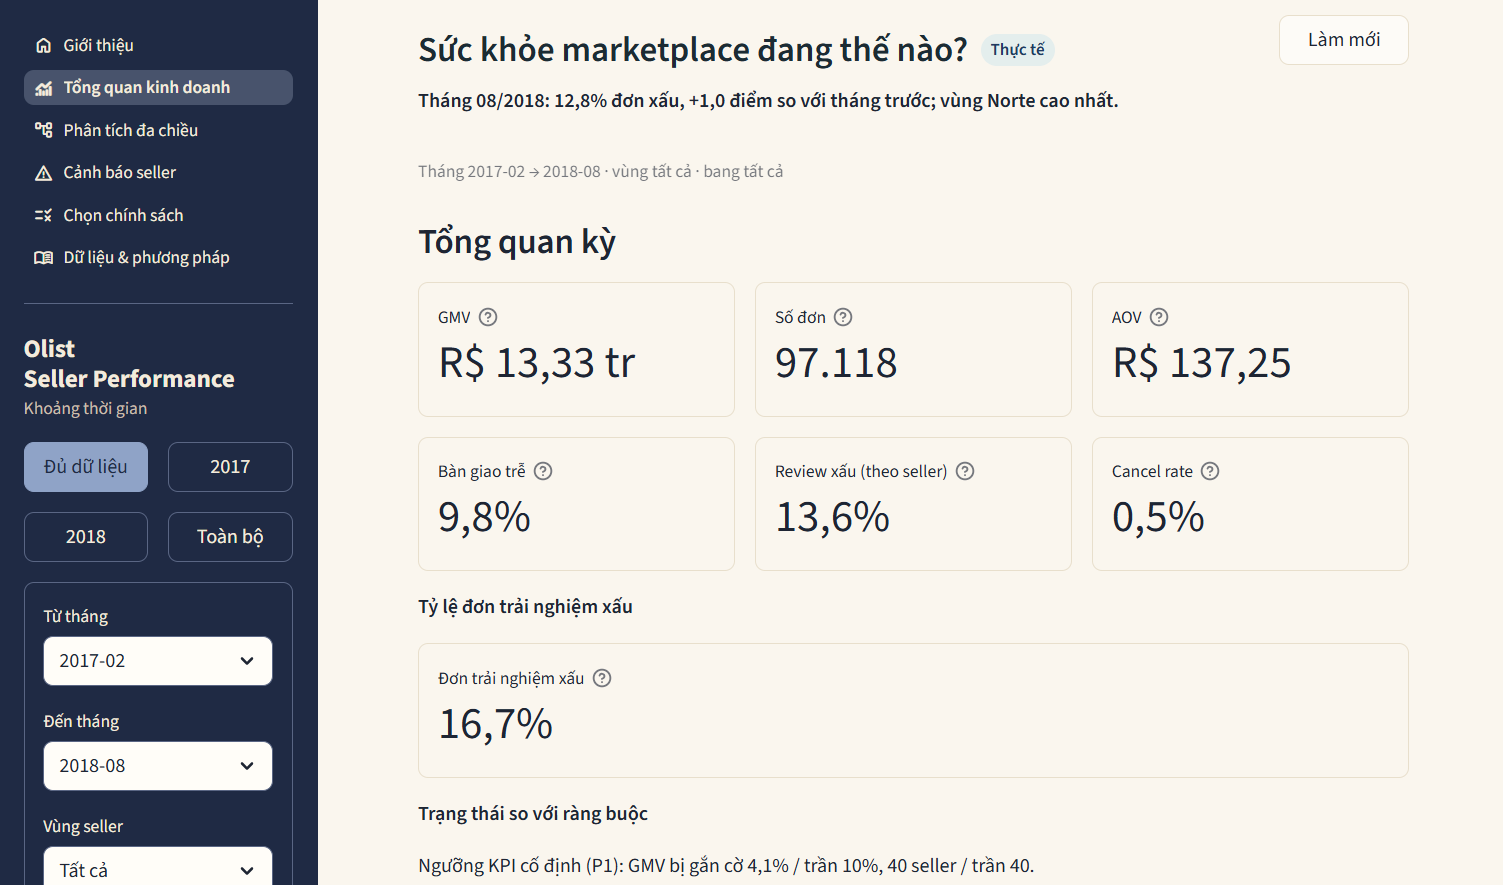
\includegraphics[width=0.92\textwidth]{images/app_kpi.png}%
}{%
  \fbox{\parbox{0.92\textwidth}{\centering\vspace{1.0cm}\textbf{[CẦN ẢNH]}~\texttt{images/app\_\allowbreak{}kpi.png}\\Giao diện trang KPI tổng quan trên Streamlit\vspace{1.0cm}}}%
}
\caption{Giao diện lớp phân tích ROLAP: trang Tổng quan kinh doanh}
\label{fig:app_kpi}
\end{figure}

Ngoài các câu hỏi cố định, trang \textit{Phân tích đa chiều} có tab \textit{Tự khám phá} cho truy vấn ad hoc. Người dùng chọn một chỉ số và một chiều trong danh sách cho phép; ứng dụng sinh câu \texttt{GROUP BY} có tham số, giới hạn 500 dòng, hiển thị câu SQL và cho tải kết quả dạng CSV. Phép cộng lại GMV theo vùng qua tab này cho đúng 13.494.400,74, bằng tổng GMV ở Mục~\ref{subsec:4_5}.

\subsection{Năm phép OLAP và phát hiện}
\label{subsec:5_2}

Năm câu hỏi Q1--Q5 tương ứng năm phép OLAP. Mỗi phép là một câu SQL cố định trên Gold, chạy trên toàn bộ cửa sổ dữ liệu; các tab này không áp bộ lọc thanh bên. Roll-up (Q1) dùng \texttt{GROUP BY ROLLUP(vùng, bang, thành phố)} trên \texttt{fact\_\allowbreak{}order\_\allowbreak{}item} để gộp tỷ lệ bàn giao trễ từ thành phố lên bang, vùng và toàn sàn trong cùng một câu. Drill-down (Q2) đi từ năm xuống quý, tháng và ngày mua trên \texttt{fact\_order} để tìm tháng có tỷ lệ review xấu nổi bật. Slice (Q3) cố định một nhóm danh mục và xếp hạng người bán theo tỷ lệ giao trễ, đếm theo đơn phân biệt vì cờ giao trễ là cờ cấp đơn. Dice (Q4) lọc đồng thời khách vùng Norte và Nordeste, quý 1--2 năm 2018 và hàng cồng kềnh, theo cách drill-across đã mô tả ở Mục~\ref{subsec:4_1}. Pivot (Q5) xoay bảng tỷ lệ bàn giao trễ từ bang người bán $\times$ quý sang nhóm danh mục $\times$ quý bằng toán tử \texttt{PIVOT}. Bảng~\ref{tab:olap_findings} tóm tắt câu hỏi và phát hiện của từng phép; mã SQL đầy đủ ở Phụ lục~\hyperref[pl:4]{PL.4}.

\begin{table}[htbp]
\centering
\footnotesize
\setlength{\tabcolsep}{3pt}
\renewcommand{\arraystretch}{1.08}
\caption{Tổng hợp năm phép OLAP, câu hỏi phân tích và phát hiện chính}
\label{tab:olap_findings}
\begin{tabularx}{\textwidth}{@{}>{\raggedright\arraybackslash}p{1.9cm}>{\raggedright\arraybackslash}p{5.2cm}>{\raggedright\arraybackslash}X@{}}
\toprule
\textbf{Phép OLAP} & \textbf{Câu hỏi phân tích} & \textbf{Phát hiện} \\
\midrule
Roll-up (Q1) & Bàn giao trễ là vấn đề của cả vùng hay của vài thành phố? & Toàn sàn 11.132/110.550 dòng hàng (10,07\%). Norte 19,2\%, Nordeste 14,4\% (1.670 dòng hàng), cao hơn mức chung; mức bang và thành phố: \textbf{[CẦN SỐ]} \\
\addlinespace
Drill-down (Q2) & Tháng nào có tỷ lệ review $\le 2$ toàn sàn nổi bật so với các tháng lân cận? & \textbf{[CẦN SỐ]} \\
\addlinespace
Slice (Q3) & Trong một nhóm danh mục, người bán nào có tỷ lệ giao trễ cao nhất? & Nhóm \texttt{electronics\_\allowbreak{}it\_\allowbreak{}telephony}: \textbf{[CẦN SỐ]} \\
\addlinespace
Dice (Q4) & Khách Norte/Nordeste, quý 1--2/2018, hàng cồng kềnh: tỷ lệ giao trễ và review xấu theo bang người bán? & 13 bang người bán có đơn thỏa điều kiện; tỷ lệ: \textbf{[CẦN SỐ]} \\
\addlinespace
Pivot (Q5) & Sau khi xem bang $\times$ quý, nhóm danh mục nào gây bàn giao trễ theo quý? & Ô cao nhất là nhóm dịch vụ và khác ở quý 4; tỷ lệ: \textbf{[CẦN SỐ]} \\
\bottomrule
\end{tabularx}
\end{table}

Phát hiện của pha \textit{Intelligence} định hướng cho các bước sau. Bàn giao trễ không phân bố đều mà tập trung hơn ở một số vùng xa trung tâm Sudeste, nên chính sách cần nhắm vào từng người bán thay vì áp một ngưỡng chung cho cả vùng. Hình~\ref{fig:olap_charts} tập hợp biểu đồ kết quả của năm phép.

\begin{figure}[htbp]
\centering
\IfFileExists{images/fig_5_2_olap_charts.png}{%
  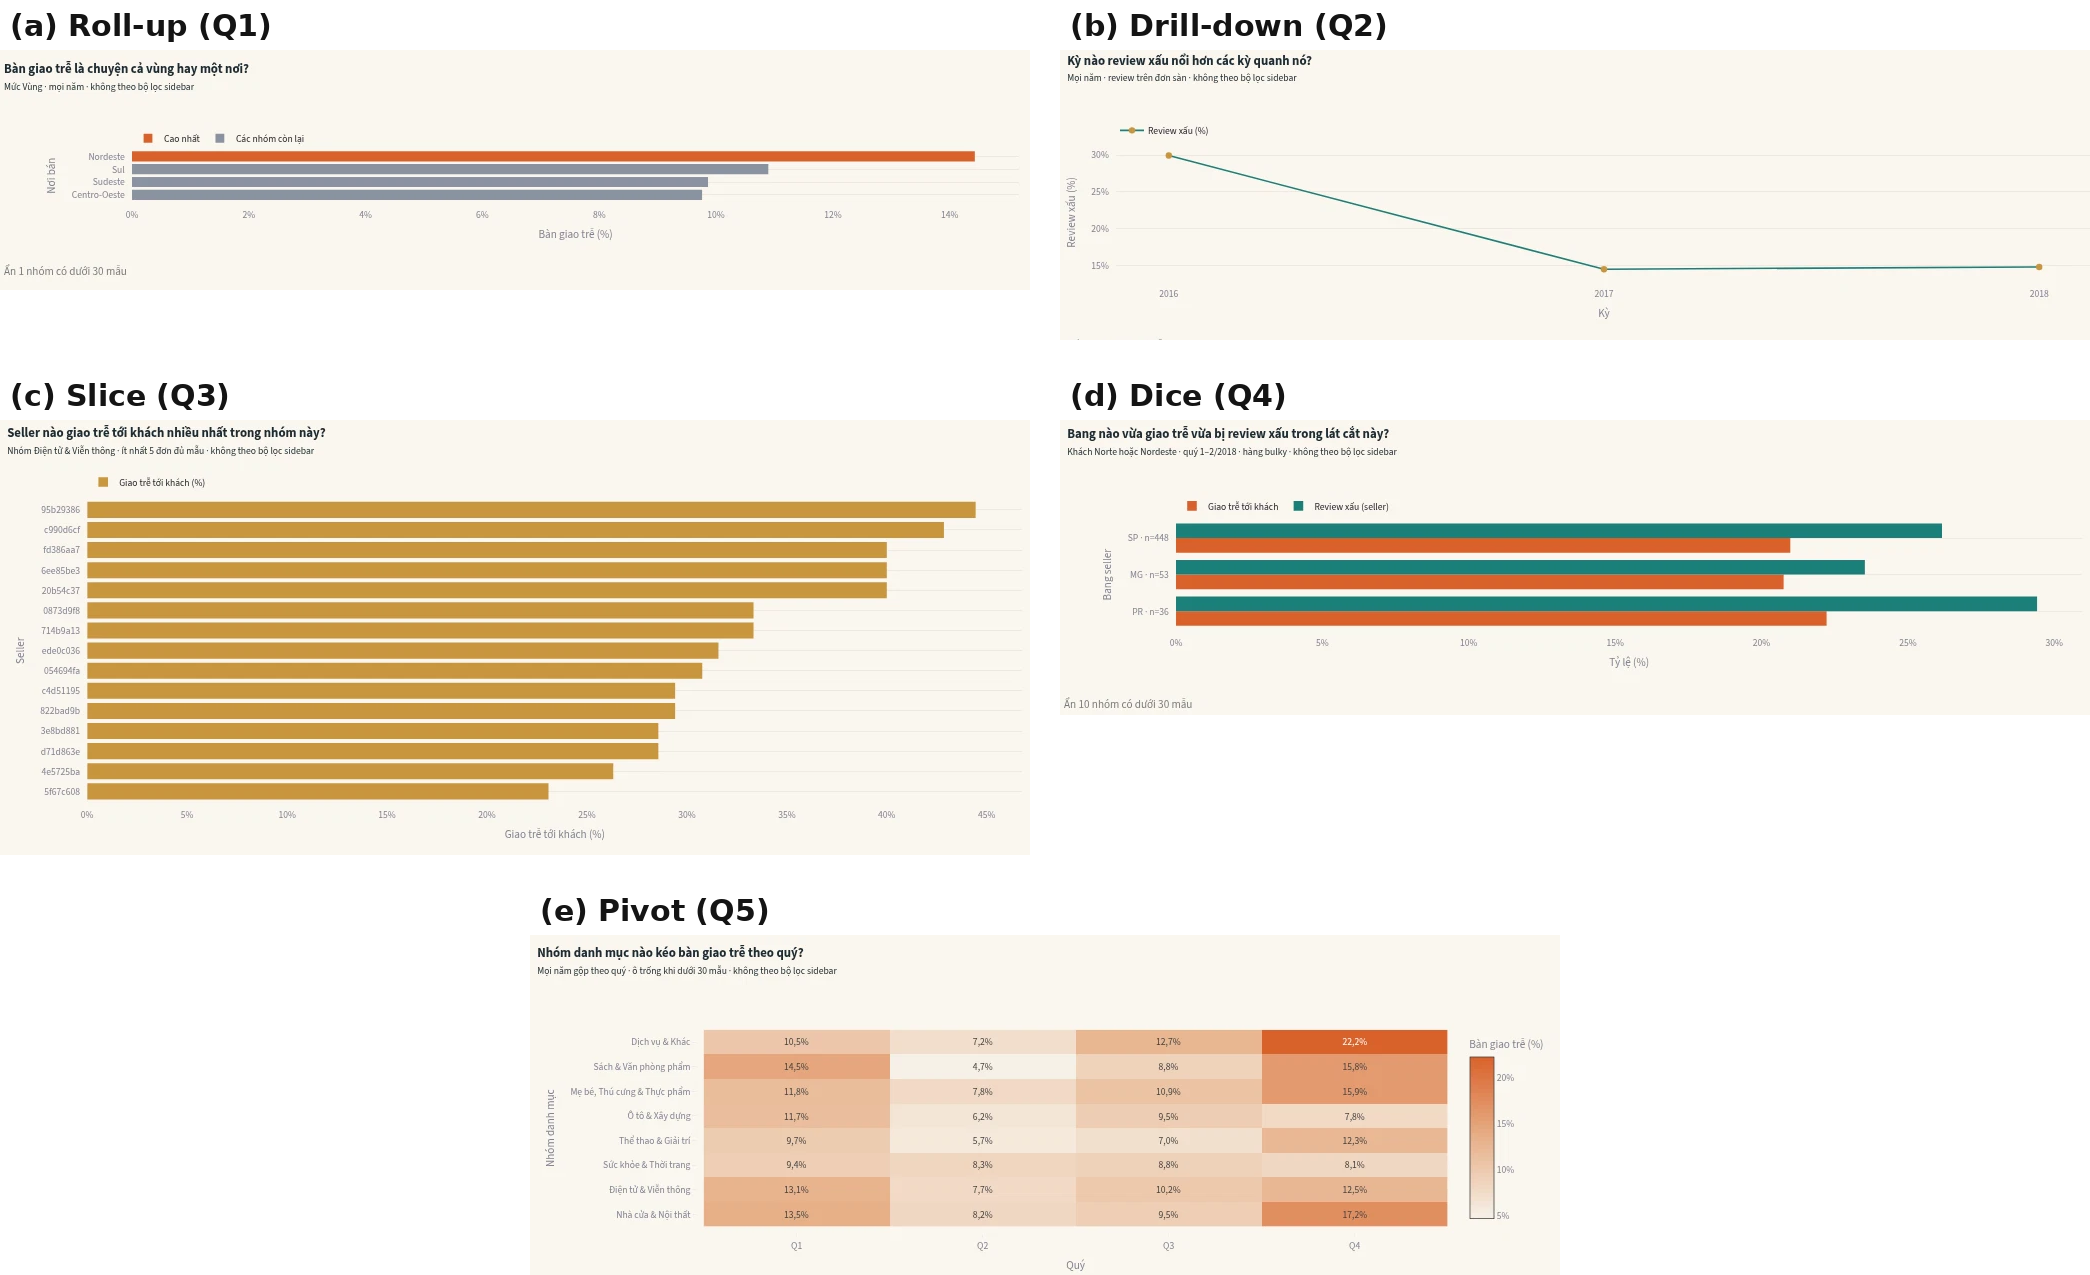
\includegraphics[width=0.92\textwidth]{images/fig_5_2_olap_charts.png}%
}{%
  \fbox{\parbox{0.92\textwidth}{\centering\vspace{1.0cm}\textbf{[CẦN ẢNH]}~\texttt{images/fig\_\allowbreak{}5\_\allowbreak{}2\_\allowbreak{}olap\_\allowbreak{}charts.png}\\Lưới 4--5 biểu đồ minh họa 5 phép OLAP\vspace{1.0cm}}}%
}
\caption{Tổng hợp biểu đồ kết quả năm phép OLAP trên trang Phân tích đa chiều}
\label{fig:olap_charts}
\end{figure}

\subsection{Kiến trúc DSS}
\label{subsec:5_3}

Hệ thống là một \textit{compound DSS}~\cite{bib:turban_dss}. Thành phần \textit{data-driven} là kho Gold và lớp OLAP ở hai mục trước. Thành phần \textit{model-driven} gồm mô hình dự báo rủi ro M1 và mô hình mô phỏng chính sách M2. Ngoài ra có một lớp luật nhẹ: mỗi hạng rủi ro được gắn sẵn một biện pháp (Bình thường, Theo dõi, Cảnh báo kèm hỗ trợ, Tạm ngưng hiển thị), và ứng dụng chỉ ra lý do khi tỷ lệ bàn giao trễ của người bán cao hơn sàn hoặc điểm review thấp hơn sàn. Lớp luật này chỉ diễn giải kết quả của M2, không tự tính lại ngưỡng hay xác suất.

Ba subsystem của DSS được hiện thực như trên Hình~\ref{fig:dss_subsystems}. \textit{Data management} là tầng Gold, view \texttt{dss.\allowbreak{}v\_\allowbreak{}seller\_\allowbreak{}features} và các bảng đầu ra trong schema \texttt{dss}. \textit{Model management} là Job DSS chạy riêng với Job ETL: Job đọc view, huấn luyện và chấm M1 cho tháng 2018-08, chạy M2 với tham số mặc định, rồi ghi đè \texttt{dss.\allowbreak{}seller\_\allowbreak{}risk\_\allowbreak{}score}, \texttt{dss.\allowbreak{}policy\_\allowbreak{}scenario} và ba bảng đánh giá mô hình (\texttt{model\_eval}, \texttt{model\_\allowbreak{}calibration}, \texttt{seller\_\allowbreak{}risk\_\allowbreak{}contrib}). Các phép what-if, goal seeking và độ nhạy chạy trực tiếp trong ứng dụng trên bảng điểm đã chấm. \textit{User interface} là ứng dụng Streamlit sáu trang; đây là thành phần duy nhất được ghi thêm dòng vào \texttt{dss.\allowbreak{}decision\_\allowbreak{}log}.

\begin{figure}[htbp]
\centering
\IfFileExists{images/fig_5_3_dss_subsystems.png}{%
  \includegraphics[width=0.85\textwidth]{images/fig_5_3_dss_subsystems.png}%
}{%
  \fbox{\parbox{0.85\textwidth}{\centering\vspace{1.0cm}\textbf{[CẦN ẢNH]}~\texttt{images/fig\_\allowbreak{}5\_\allowbreak{}3\_\allowbreak{}dss\_\allowbreak{}subsystems.png}\\Ba subsystem của hệ thống DSS (Data, Model, UI)\vspace{1.0cm}}}%
}
\caption{Kiến trúc ba thành phần (subsystem) của hệ hỗ trợ quyết định}
\label{fig:dss_subsystems}
\end{figure}

Tháng chấm được cố định là 2018-08 chứ không lấy tháng lớn nhất trong dữ liệu. Hai tháng 2018-09 và 2018-10 quá thưa; nếu lấy tháng lớn nhất, bảng điểm chỉ còn đúng 1 người bán. Tháng 2018-08 có 1.278 người bán hoạt động với 6.540 đơn hợp lệ, trong đó 342 người bán có từ 5 đơn hợp lệ trở lên. Kết quả dự báo vì vậy là cho tháng kế tiếp 2018-09, theo kiểu mô phỏng một bước về phía trước trên dữ liệu lịch sử. Bảng~\ref{tab:simon_app_map} ánh xạ bốn pha ra quyết định với chức năng DSS và trang ứng dụng.

\begin{table}[htbp]
\centering
\footnotesize
\setlength{\tabcolsep}{3pt}
\renewcommand{\arraystretch}{1.08}
\caption{Ánh xạ pha ra quyết định Simon với chức năng DSS và trang ứng dụng}
\label{tab:simon_app_map}
\begin{tabularx}{\textwidth}{@{}>{\raggedright\arraybackslash}p{2.3cm}>{\raggedright\arraybackslash}X>{\raggedright\arraybackslash}p{4.2cm}@{}}
\toprule
\textbf{Pha Simon} & \textbf{Chức năng DSS} & \textbf{Trang ứng dụng Streamlit} \\
\midrule
Intelligence & KPI toàn sàn, xu hướng, bản đồ bang; năm phép OLAP và truy vấn ad hoc để xác định vấn đề và mức độ & Tổng quan kinh doanh; Phân tích đa chiều \\
\addlinespace
Design & Điểm rủi ro M1 cho từng người bán, phân bố điểm, đóng góp từng đặc trưng, độ tin cậy mô hình; định nghĩa P0, P1, P2 & Cảnh báo seller; Dữ liệu \& phương pháp \\
\addlinespace
Choice & So sánh P0/P1/P2 theo M2, what-if trên giả định, goal seeking, budget seeking, độ nhạy tornado, khuyến nghị theo nguyên tắc chọn & Chọn chính sách \\
\addlinespace
Implementation & Chốt phương án, ghi một dòng vào \texttt{dss.\allowbreak{}decision\_\allowbreak{}log}, tải danh sách người bán bị gắn cờ (CSV) & Chọn chính sách (nút Chốt) \\
\bottomrule
\end{tabularx}
\end{table}

\subsection{Influence diagram và hệ thống biến}
\label{subsec:5_4}

Hình~\ref{fig:influence_diagram} là influence diagram của bài toán can thiệp người bán~\cite{bib:turban_dss}. Ba nút quyết định là ngưỡng điểm rủi ro, ngưỡng KPI cứng và biện pháp theo hạng. Lịch sử hiệu suất trong kho xác định điểm rủi ro $p_i$; điểm rủi ro cùng các ngưỡng xác định hạng của người bán. Hạng và hiệu quả can thiệp quyết định số đơn xấu tránh được; hạng, nhu cầu và tỷ lệ chuyển đơn quyết định phần GMV bị ảnh hưởng. Ba nút kết quả là số đơn trải nghiệm xấu dự kiến, GMV bị ảnh hưởng và số người bán cần xử lý.

\begin{figure}[htbp]
\centering
\IfFileExists{images/fig_5_4_influence_diagram.png}{%
  \includegraphics[width=0.88\textwidth]{images/fig_5_4_influence_diagram.png}%
}{%
  \fbox{\parbox{0.88\textwidth}{\centering\vspace{1.0cm}\textbf{[CẦN ẢNH]}~\texttt{images/fig\_\allowbreak{}5\_\allowbreak{}4\_\allowbreak{}influence\_\allowbreak{}diagram.png}\\Influence diagram của mô hình quyết định\vspace{1.0cm}}}%
}
\caption{Influence diagram mô tả quan hệ các biến trong DSS}
\label{fig:influence_diagram}
\end{figure}

Bảng~\ref{tab:dss_variables} phân loại các biến theo bốn nhóm. Các giá trị mặc định là quy ước của nhóm, không phải số đo; người dùng chỉnh được trên ứng dụng. Riêng $X = 10\%$ và $N = 40$ là ràng buộc cố định của bài toán. Danh sách tham số đầy đủ ở Phụ lục~\hyperref[pl:6]{PL.6}.

\begin{table}[htbp]
\centering
\footnotesize
\setlength{\tabcolsep}{3pt}
\renewcommand{\arraystretch}{1.1}
\caption{Phân loại các biến trong mô hình DSS}
\label{tab:dss_variables}
\begin{tabularx}{\textwidth}{@{}>{\raggedright\arraybackslash}p{2.3cm}>{\raggedright\arraybackslash}p{5.0cm}>{\raggedright\arraybackslash}X@{}}
\toprule
\textbf{Nhóm biến} & \textbf{Ký hiệu / Tên biến} & \textbf{Ý nghĩa và giá trị mặc định} \\
\midrule
Quyết định & $\theta_1, \theta_2, \theta_3$ & Ngưỡng xác suất của hạng 1, 2, 3 trong P2; mặc định 0,20; 0,35; 0,50 \\
 & Ngưỡng KPI cứng của P1 & Gắn cờ khi tỷ lệ bàn giao trễ $\ge 0{,}15$ hoặc điểm review trung bình $\le 3{,}5$ \\
 & \texttt{min\_orders} & Số đơn hợp lệ tối thiểu trong tháng để được xếp hạng; mặc định 5 \\
 & Chính sách $\pi \in \{\text{P0}, \text{P1}, \text{P2}\}$ & Phương án được chọn và biện pháp gắn với từng hạng \\
\addlinespace
Không kiểm soát & $e_k$ & Hiệu quả can thiệp ở hạng $k$: 0,25; 0,50; 0,75; P1 dùng 0,50 \\
 & $r$ & Tỷ lệ GMV của người bán bị gắn cờ chuyển sang người bán khác; mặc định 0,5 \\
 & $s$ & Hệ số mùa vụ của nhu cầu tháng tới; mặc định 1,0 \\
 & Lịch sử hiệu suất & Đặc trưng người bán đọc từ Gold, đầu vào của M1 \\
\addlinespace
Trung gian & $p_i$ & Xác suất một đơn tháng tới của người bán $i$ là đơn trải nghiệm xấu (M1) \\
 & $Q_i = \bar{Q}_i \cdot s$ & Số đơn dự kiến; $\bar{Q}_i$ là số đơn hợp lệ của tháng chấm \\
 & $k(i)$ & Hạng của người bán $i$ theo chính sách \\
\addlinespace
Kết quả & $E[B]$ & Số đơn trải nghiệm xấu dự kiến (mục tiêu cực tiểu) \\
 & $G$ & Phần trăm GMV bị ảnh hưởng (ràng buộc $\le X$) \\
 & $n_{\text{flag}}$ & Số người bán bị gắn cờ (ràng buộc $\le N$) \\
\bottomrule
\end{tabularx}
\end{table}

Theo phân loại ở Mục~\ref{subsec:2_4}, M1 là mô hình tĩnh trong điều kiện \textit{risk}, vì nó ước lượng xác suất từ dữ liệu lịch sử. Ngược lại, $e_k$ và $r$ chưa từng được đo trên Olist nên thuộc điều kiện \textit{uncertainty}; hệ thống xử lý chúng bằng kịch bản what-if và phân tích độ nhạy thay vì coi là số chắc chắn.

\subsection{M1: Dự báo rủi ro người bán}
\label{subsec:5_5}

M1 ước lượng $p_i$, xác suất một đơn của người bán $i$ ở tháng $t+1$ là đơn trải nghiệm xấu, bằng hồi quy logistic theo Phương trình~\eqref{eq:sigmoid}~\cite{bib:sklearn}. Đơn vị quan sát là một cặp người bán--tháng trong \texttt{dss.\allowbreak{}v\_\allowbreak{}seller\_\allowbreak{}features}. Đặc trưng ở tháng $t$ gồm năm biến số: trung bình tỷ lệ bàn giao trễ ba tháng gần nhất, điểm review trung bình, số đơn hợp lệ, khoảng cách giao trung bình và tuổi người bán tính từ ngày ký deal; cùng hai biến phân loại mã hóa one-hot: nhóm danh mục chiếm nhiều dòng hàng nhất trong tháng và vùng của người bán. Giá trị số bị thiếu được điền bằng trung vị của tập huấn luyện.

Nhãn lấy từ tháng lịch kế tiếp của cùng người bán: số đơn trải nghiệm xấu trên số đơn đủ điều kiện ở tháng $t+1$. Để hàm mất mát khớp với phân phối nhị thức, mỗi cặp người bán--tháng được mở rộng thành từng đơn: một người bán có 20 đơn đủ điều kiện, trong đó 3 đơn xấu, đóng góp 3 dòng nhãn 1 và 17 dòng nhãn 0. Tập huấn luyện chỉ gồm người bán có ít nhất 10 dòng hàng hợp lệ trong ít nhất sáu tháng, để mô hình học từ lịch sử đủ dài. Dữ liệu được chia theo thời gian, không chia ngẫu nhiên: hai tháng cuối có nhãn trước tháng chấm làm tập kiểm thử, các tháng trước đó làm tập huấn luyện, nên mô hình không nhìn thấy tương lai. Nếu không đủ tháng có nhãn, dữ liệu chỉ có một lớp, hoặc thuật toán không hội tụ, Job chuyển sang mô hình cơ sở: điểm của mỗi người bán là tỷ lệ đơn xấu của chính người bán đó trong tháng chấm.

Mô hình được đánh giá trên các đơn của tập kiểm thử bằng ba chỉ số ở Mục~\ref{subsec:2_4}: AUC-ROC đo khả năng xếp hạng, Brier score đo sai số của xác suất, và đồ thị hiệu chuẩn so xác suất dự báo trung bình với tỷ lệ thực tế trong mười nhóm thập phân vị. Hiệu chuẩn quan trọng hơn AUC trong bài toán này, vì M2 nhân trực tiếp $p_i$ với số đơn dự kiến. Kết quả ở Bảng~\ref{tab:m1_metrics} và Hình~\ref{fig:m1_calibration}.

\begin{table}[htbp]
\centering
\footnotesize
\caption{Chỉ số đánh giá mô hình dự báo M1 trên tập kiểm thử}
\label{tab:m1_metrics}
\begin{tabular}{ll}
\toprule
\textbf{Chỉ số} & \textbf{Giá trị đo được} \\
\midrule
Tháng kiểm thử & \textbf{[CẦN SỐ]} \\
Số đơn huấn luyện $n_{\text{train}}$ / kiểm thử $n_{\text{test}}$ & \textbf{[CẦN SỐ]} / \textbf{[CẦN SỐ]} \\
Tỷ lệ đơn xấu cơ sở (base rate) & \textbf{[CẦN SỐ]} \\
ROC-AUC & \textbf{[CẦN SỐ]} \\
Brier score & \textbf{[CẦN SỐ]} \\
\bottomrule
\end{tabular}
\end{table}

\begin{figure}[htbp]
\centering
\IfFileExists{images/fig_5_5_calibration.png}{%
  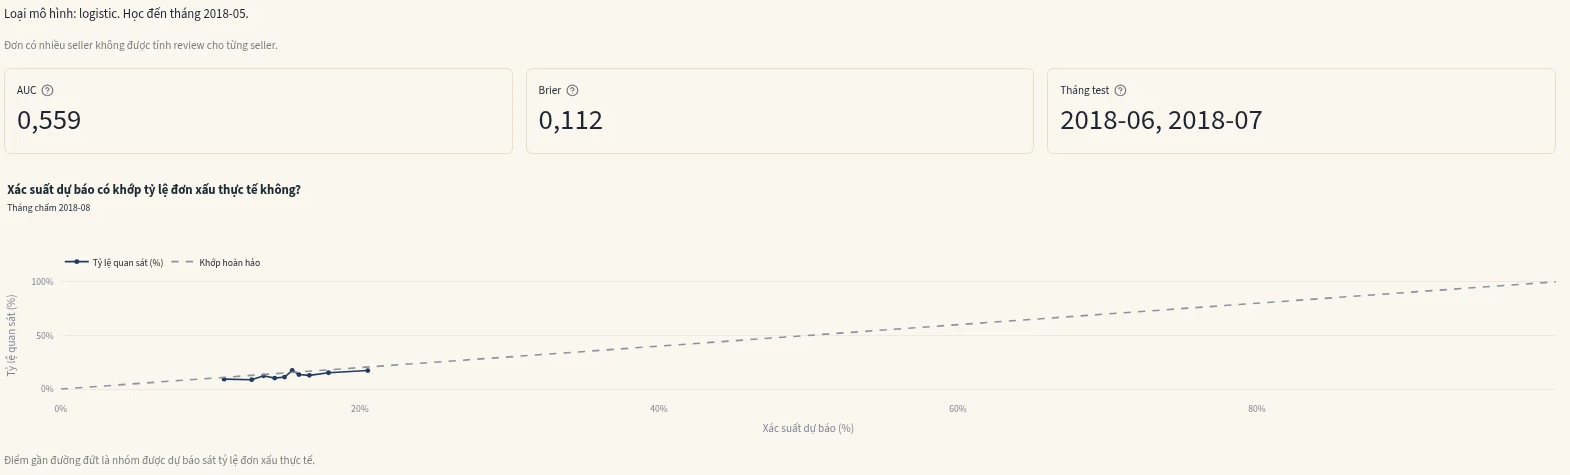
\includegraphics[width=0.80\textwidth]{images/fig_5_5_calibration.png}%
}{%
  \fbox{\parbox{0.80\textwidth}{\centering\vspace{1.0cm}\textbf{[CẦN ẢNH / CẦN SỐ]}~\texttt{images/fig\_\allowbreak{}5\_\allowbreak{}5\_\allowbreak{}calibration.png}\\Đồ thị calibration của mô hình M1 theo 10 bin\vspace{1.0cm}}}%
}
\caption{Đồ thị hiệu chuẩn (calibration plot) của mô hình M1}
\label{fig:m1_calibration}
\end{figure}

Để người quản lý hiểu vì sao một người bán bị chấm điểm cao, Job tính đóng góp của từng đặc trưng vào logit: $c_{ij} = \beta_j (x_{ij} - \bar{x}_j)$, với $\bar{x}_j$ là trung bình trên tập huấn luyện; tổng các đóng góp cộng hệ số chặn đã hiệu chỉnh đúng bằng logit của người bán. Tab \textit{Chi tiết seller} trên trang Cảnh báo seller hiển thị các đóng góp này. Mô hình có hai hạn chế cần nêu. Thứ nhất, tập huấn luyện chỉ gồm người bán có lịch sử dài, trong khi tháng chấm gồm cả 1.278 người bán đang hoạt động, nên phân phối dữ liệu lúc chấm khác lúc học. Thứ hai, đặc trưng số chưa được chuẩn hóa trước khi dùng điều chuẩn L2 mặc định, nên độ lớn hệ số không so sánh trực tiếp được giữa các đặc trưng.

\subsection{M2: Mô phỏng chính sách}
\label{subsec:5_6}

M2 nhận bảng điểm của tháng chấm và tính kết quả của một chính sách $\pi$ trong một kỳ. Chỉ người bán có $\bar{Q}_i \ge \texttt{min\_orders}$ được xếp hạng. P0 không gắn cờ ai và là mốc so sánh. P1 gắn cờ người bán có tỷ lệ bàn giao trễ $\ge 0{,}15$ hoặc điểm review trung bình $\le 3{,}5$, với một mức hiệu quả chung $e_{P1}$. P2 xếp người bán vào ba hạng theo xác suất M1:
\begin{equation}
\label{eq:tier}
k(i) =
\begin{cases}
3 & \text{nếu } p_i \ge \theta_3,\\
2 & \text{nếu } \theta_2 \le p_i < \theta_3,\\
1 & \text{nếu } \theta_1 \le p_i < \theta_2,\\
0 & \text{ngược lại.}
\end{cases}
\end{equation}
Nếu số người bán bị gắn cờ vượt $N$, mô hình chỉ giữ $N$ người bán nặng nhất (theo $p_i$ với P2, theo tỷ lệ bàn giao trễ với P1). Số đơn trải nghiệm xấu dự kiến và phần GMV bị ảnh hưởng là:
\begin{equation}
\label{eq:expected_bad}
E[B](\pi) = \sum_{i} p_i \, Q_i \, \bigl(1 - e_{k(i)}\bigr), \qquad Q_i = \bar{Q}_i \cdot s,
\end{equation}
\begin{equation}
\label{eq:gmv_affected}
G(\pi) = 100 \times \frac{\sum_{i \in F(\pi)} \text{gmv}_i \, (1 - r)}{\sum_{i} \text{gmv}_i},
\end{equation}
trong đó $F(\pi)$ là tập người bán bị gắn cờ, $e_0 = 0$, và tổng ở mẫu số chạy trên mọi người bán được chấm trong tháng. Trong mã hiện tại, Phương trình~\eqref{eq:gmv_affected} tính GMV bị ảnh hưởng cho mọi người bán bị gắn cờ, kể cả hạng Theo dõi, chứ không chỉ người bán bị tạm ngưng hiển thị; cách tính này thận trọng, có xu hướng ước lượng cao phần GMV bị ảnh hưởng.
% TODO kiểm tra GMV ảnh hưởng: đặc tả ghi chỉ tính seller bị tạm ngưng; code policy.simulate tính gmv*(1-r) cho mọi seller bị gắn cờ, mẫu số là tổng GMV của seller được chấm tháng 2018-08.
Nguyên tắc chọn là cực tiểu $E[B]$ với ràng buộc $G \le X = 10\%$ và $n_{\text{flag}} \le N = 40$. Ứng dụng khuyến nghị phương án khả thi (khác P0) có $E[B]$ nhỏ nhất.

Bảng~\ref{tab:m2_policies} so sánh ba phương án với tham số mặc định. Với P2, 7 trong 342 người bán đủ điều kiện bị gắn cờ, cả 7 đều ở hạng Theo dõi, ảnh hưởng 0,3\% GMV và đạt cả hai ràng buộc. Tuy nhiên số đơn xấu dự kiến chỉ giảm từ 685,2 xuống 682,0, khoảng 0,5\%. Nguyên nhân là phần lớn xác suất $p_i$ nằm dưới ngưỡng mặc định $\theta_1 = 0{,}20$, nên rất ít người bán bị can thiệp; ngưỡng mặc định là quá chặt so với phân phối điểm thực tế, và đây chính là lý do cần công cụ goal seeking.
% Số P0/P2 đọc trên app với bảng điểm 2018-08 hiện có; cần xác nhận lại bằng dss.policy_scenario sau lần chạy Job DSS cuối.

\begin{table}[htbp]
\centering
\footnotesize
\caption{So sánh kết quả mô phỏng các chính sách P0, P1 và P2 (tham số mặc định, tháng chấm 2018-08)}
\label{tab:m2_policies}
\begin{tabular}{lrrr}
\toprule
\textbf{Chính sách} & \textbf{Số seller gắn cờ} & \textbf{\% GMV bị ảnh hưởng} & \textbf{$E[B]$ (đơn xấu dự kiến)} \\
\midrule
P0 (Không can thiệp) & 0 & 0\% & 685,2 \\
P1 (Ngưỡng KPI cố định) & \textbf{[CẦN SỐ]} & \textbf{[CẦN SỐ]} & \textbf{[CẦN SỐ]} \\
P2 (Theo xác suất M1) & 7 & 0,3\% & 682,0 \\
\bottomrule
\end{tabular}
\end{table}

Ứng dụng cung cấp ba kỹ thuật phân tích kịch bản~\cite{bib:turban_dss}. \textit{What-if}: người dùng chỉnh $\theta$, $e_k$, $r$, $s$, ngưỡng KPI và \texttt{min\_orders} trong tab Giả định, mọi kết quả tính lại ngay. \textit{Goal seeking}: tìm $\theta_1$ nhỏ nhất trong $[0; 0{,}70]$, giữ $\theta_2 = \theta_1 + 0{,}15$ và $\theta_3 = \theta_1 + 0{,}30$, sao cho $G \le X$, bằng phương pháp chia đôi với sai số $10^{-4}$; ràng buộc $N$ luôn được giữ nhờ bước cắt ở trên. Kết quả goal seeking với tham số mặc định là $\theta_1 = $ \textbf{[CẦN SỐ]}, ảnh hưởng \textbf{[CẦN SỐ]}\% GMV và \textbf{[CẦN SỐ]} người bán. \textit{Budget seeking} xếp người bán đủ điều kiện theo $p_i$ giảm dần và tìm số $k \le N$ lớn nhất mà GMV bị ảnh hưởng cộng dồn chưa vượt $X$, đồng thời cho biết ràng buộc nào chặn trước ($X$ hay $N$); kết quả: $k = $ \textbf{[CẦN SỐ]}, ràng buộc chặn \textbf{[CẦN SỐ]}. Cuối cùng, \textit{phân tích độ nhạy} nhân lần lượt $e_k$ (cả ba hạng), $r$ và $s$ với 0,8 và 1,2 rồi tính lại P2; Hình~\ref{fig:m2_tornado} cho thấy giả định nào làm kết quả dao động mạnh nhất (giá trị thấp/cao: \textbf{[CẦN SỐ]}). Vì $s$ nhân thẳng vào $Q_i$, $E[B]$ thay đổi tỷ lệ thuận với $s$; còn $r$ chỉ tác động đến GMV bị ảnh hưởng, không đến số đơn xấu.

\begin{figure}[htbp]
\centering
\IfFileExists{images/fig_5_6_tornado.png}{%
  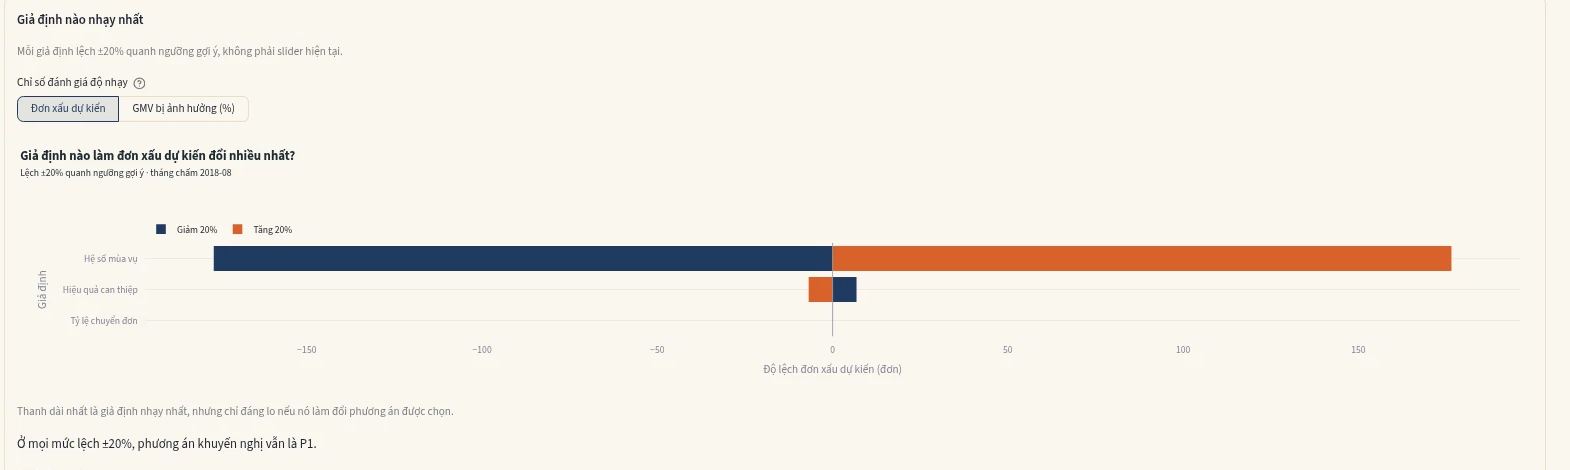
\includegraphics[width=0.82\textwidth]{images/fig_5_6_tornado.png}%
}{%
  \fbox{\parbox{0.82\textwidth}{\centering\vspace{1.0cm}\textbf{[CẦN ẢNH / CẦN SỐ]}~\texttt{images/fig\_\allowbreak{}5\_\allowbreak{}6\_\allowbreak{}tornado.png}\\Biểu đồ Tornado độ nhạy $\pm 20\%$ cho $e_k, r, s$\vspace{1.0cm}}}%
}
\caption{Phân tích độ nhạy tornado của P2 đối với các giả định $e_k$, $r$, $s$ ($\pm 20\%$)}
\label{fig:m2_tornado}
\end{figure}

\subsection{Ứng dụng và triển khai}
\label{subsec:5_7}

Ứng dụng Streamlit có sáu trang, mỗi trang mở đầu bằng một câu hỏi và một câu kết luận sinh từ dữ liệu, kèm nhãn cho biết số trên trang là thực tế (từ Gold) hay dự báo (từ M1, M2). Trang \textit{Giới thiệu} nêu bối cảnh, ba KPI toàn sàn, hai ràng buộc $X$, $N$ và lối vào bốn trang câu hỏi. \textit{Tổng quan kinh doanh} và \textit{Phân tích đa chiều} phục vụ pha \textit{Intelligence}. \textit{Cảnh báo seller} trả lời ``người bán nào đáng lo nhất'' với bốn tab Danh sách, Phân bố, Chi tiết seller và Độ tin cậy. \textit{Chọn chính sách} (Hình~\ref{fig:app_policy}) đặt thẻ khuyến nghị và nút Chốt ở đầu trang, các tab bên dưới chứa lập luận của M2: ngưỡng tối ưu, độ tin cậy của kết quả và giả định. \textit{Dữ liệu \& phương pháp} trình bày nguồn dữ liệu, dòng chảy dữ liệu, giới hạn và giả định của M1, M2.

\begin{figure}[htbp]
\centering
\IfFileExists{images/app_policy.png}{%
  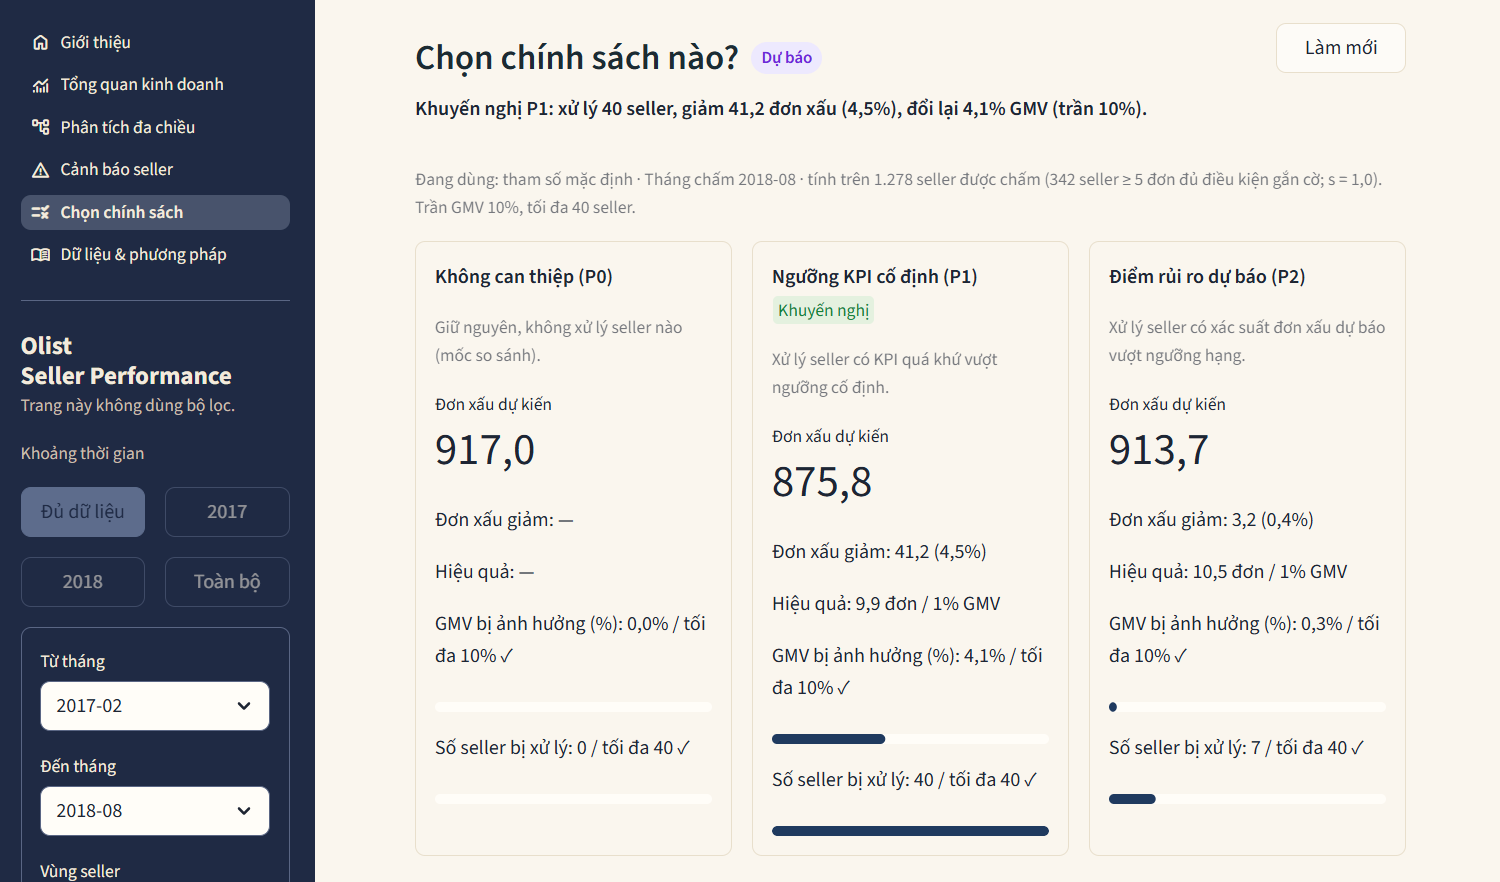
\includegraphics[width=0.92\textwidth]{images/app_policy.png}%
}{%
  \fbox{\parbox{0.92\textwidth}{\centering\vspace{1.0cm}\textbf{[CẦN ẢNH]}~\texttt{images/app\_\allowbreak{}policy.png}\\Giao diện trang chọn chính sách trên Streamlit\vspace{1.0cm}}}%
}
\caption{Giao diện trang Chọn chính sách (M2 và ghi \texttt{decision\_log})}
\label{fig:app_policy}
\end{figure}

Kịch bản sử dụng của người quản lý gồm năm bước: xem sức khỏe sàn trên trang tổng quan, tìm nơi phát sinh vấn đề bằng OLAP, xem danh sách người bán rủi ro tháng tới, so sánh và điều chỉnh chính sách, rồi chốt quyết định. Khi bấm Chốt, ứng dụng hiện hộp xác nhận, sinh mã \texttt{decision\_id} dạng UUID và ghi thêm một dòng vào \texttt{dss.\allowbreak{}decision\_\allowbreak{}log} qua SQL Warehouse. Dòng này lưu tháng chấm, phương án đã chọn, toàn bộ tham số ($\theta$, $e_k$, $r$, $s$, ngưỡng KPI, \texttt{min\_orders}, $X$, $N$), kết quả ($E[B]$, $G$, số người bán) và ghi chú. Một khóa trong phiên làm việc ngăn việc ghi trùng khi người dùng bấm nhiều lần. Người dùng cũng tải được danh sách người bán bị gắn cờ dạng CSV để chuyển cho bộ phận vận hành. Sau buổi demo, bảng \texttt{decision\_log} có \textbf{[CẦN SỐ]} dòng.

Ứng dụng được triển khai trên Streamlit Community Cloud tại \url{https://olist-dw-dss.streamlit.app/}. Thông tin kết nối warehouse (host, HTTP path, token) được đọc theo thứ tự \texttt{st.secrets}, biến môi trường, rồi tệp \texttt{.env}; tệp bí mật không được đưa vào kho mã, và thông báo lỗi không in ra token. Bộ kiểm thử tự động bằng \texttt{pytest} cho mô hình M2, phần sinh câu kết luận và lớp truy vấn gồm 38 ca, cả 38 ca đều đạt.

%%%%%%%%%%%%%%%%%%%%%%%%%%%%%%%%%
% CHƯƠNG 6
%%%%%%%%%%%%%%%%%%%%%%%%%%%%%%%%%
\section{Đánh giá, hạn chế và hướng phát triển}
\label{sec:ch6}

\subsection{Đối chiếu yêu cầu đề}
\label{subsec:6_1}

Đề bài đặt sáu mục tiêu và ba điều kiện cho đề tài: kho dữ liệu phải là cốt lõi, dữ liệu phải hợp lệ và đủ lớn, và bài toán phải có ý nghĩa thực tế. Bảng~\ref{tab:rtm_checklist} đối chiếu từng yêu cầu với mục đáp ứng trong báo cáo và bằng chứng trong hệ thống. Trạng thái ``Đạt, còn bổ sung số'' nghĩa là chức năng đã chạy nhưng một số kết quả đo còn chờ lần chạy cuối.

\begin{table}[htbp]
\centering
\footnotesize
\setlength{\tabcolsep}{3pt}
\renewcommand{\arraystretch}{1.08}
\caption{Checklist đối chiếu mục tiêu đề bài và các yêu cầu bắt buộc}
\label{tab:rtm_checklist}
\begin{tabularx}{\textwidth}{@{}>{\raggedright\arraybackslash}p{3.3cm}>{\raggedright\arraybackslash}p{1.9cm}>{\raggedright\arraybackslash}X>{\raggedright\arraybackslash}p{1.9cm}@{}}
\toprule
\textbf{Yêu cầu của đề} & \textbf{Nơi đáp ứng} & \textbf{Bằng chứng trong hệ thống} & \textbf{Trạng thái} \\
\midrule
1. Phân tích nghiệp vụ & Mục~\ref{subsec:1_1}--\ref{subsec:1_3} & Người ra quyết định, chu kỳ tháng, ba phương án, nguyên tắc chọn và hai ràng buộc $X$, $N$; mười câu hỏi Q1--Q10 gắn KPI và dimension & Đạt \\
\addlinespace
2. Thiết kế DW đa chiều kèm ETL & Mục~\ref{subsec:4_1}--\ref{subsec:4_4} & Fact constellation 3 fact, 7 dimension, grain khai báo cho từng fact, phân cấp, bus matrix; pipeline Bronze--Silver--Gold & Đạt \\
\addlinespace
3. Backend và frontend & Mục~\ref{subsec:4_4}, \ref{subsec:5_1}, \ref{subsec:5_2}, \ref{subsec:5_7} & Delta Lake và Unity Catalog; Job ETL sáu task; năm phép OLAP bằng SQL trên SQL Warehouse; ứng dụng Streamlit sáu trang có bộ lọc, KPI, truy vấn ad hoc & Đạt, còn bổ sung số \\
\addlinespace
4. Thành phần DSS dựa trên DW & Mục~\ref{subsec:5_3}--\ref{subsec:5_6} & M1 huấn luyện từ view trên Gold, M2 mô phỏng P0/P1/P2; đủ ba thành phần dữ liệu, mô hình, giao diện; influence diagram, bảng biến, ánh xạ pha Simon; what-if, goal seeking, phân tích độ nhạy & Đạt, còn bổ sung số \\
\addlinespace
5. Đánh giá, hạn chế, hướng phát triển & Chương~\ref{sec:ch6} & Bảng kiểm chứng DW, M1, M2; danh sách hạn chế và bài học; hướng phát triển & Đạt \\
\addlinespace
6. Thuyết trình & Ngoài báo cáo & Slide và buổi trình bày của nhóm & Thực hiện riêng \\
\midrule
DW là cốt lõi & Mục~\ref{subsec:3_4}, \ref{subsec:3_5} & OLAP, M1 và M2 đều đọc từ Gold; Job ETL và Job DSS tách riêng; ứng dụng không đọc CSV thô & Đạt \\
\addlinespace
Dữ liệu hợp lệ, đủ lớn & Mục~\ref{subsec:3_1}, \ref{subsec:3_3} & Dữ liệu công khai trên Kaggle, giấy phép CC BY-NC-SA 4.0; 12 tệp nguồn, 99.441 đơn, 112.650 dòng hàng, 1.000.163 điểm địa lý; có lỗi dữ liệu thật để làm sạch & Đạt \\
\addlinespace
Ý nghĩa thực tế & Mục~\ref{subsec:1_2} & Quyết định can thiệp người bán hằng tháng, có tiêu chuẩn chọn đo được và ghi lại quyết định đã chốt & Đạt \\
\bottomrule
\end{tabularx}
\end{table}

\subsection{Đánh giá kết quả}
\label{subsec:6_2}

\textbf{Kho dữ liệu.} Số liệu trên Gold khớp với nguồn. \texttt{fact\_order} có 99.441 dòng, bằng số đơn trong tệp; \texttt{dim\_seller} có 3.095 người bán và \texttt{dim\_customer} có 96.096 khách, khớp số mã phân biệt của nguồn. Tổng GMV bằng 13.494.400,74 theo cả ba cách cộng (theo tháng, theo vùng người bán, trực tiếp từ dòng hàng), nên measure cộng được không bị mất hay nhân đôi qua các phân cấp. Ràng buộc \texttt{CHECK} và \texttt{NOT NULL} làm lệnh ghi thất bại nếu có dòng vi phạm, nên dữ liệu sai không lặng lẽ đi vào kho (Mục~\ref{subsec:4_5}). Tính idempotent chưa có số đo hai lần chạy liên tiếp (\textbf{[CẦN SỐ]}); theo thiết kế, \texttt{MERGE} theo grain không có nhánh xóa và khóa thay thế được cấp tất định, nên chạy lại cùng dữ liệu không sinh thêm dòng.

\textbf{Mô hình M1.} M1 chỉ có giá trị nếu tốt hơn mô hình đoán mọi đơn bằng tỷ lệ cơ sở. Với mô hình đó, AUC bằng 0,5 và Brier xấp xỉ $b(1-b)$, với $b$ là tỷ lệ đơn xấu cơ sở. Trên tập kiểm thử, M1 đạt AUC \textbf{[CẦN SỐ]} và Brier \textbf{[CẦN SỐ]}, so với mốc Brier \textbf{[CẦN SỐ]} của tỷ lệ cơ sở; đồ thị hiệu chuẩn ở Hình~\ref{fig:m1_calibration}.

\textbf{Mô hình M2.} Với tham số mặc định, P2 gắn cờ 7 trong 342 người bán đủ điều kiện, ảnh hưởng 0,3\% GMV và đạt cả hai ràng buộc. Số đơn xấu dự kiến giảm từ 685,2 (P0) xuống 682,0, tức khoảng 0,5\%. Kết quả của P1 là \textbf{[CẦN SỐ]}. Mức giảm nhỏ không cho thấy mô hình sai mà cho thấy ngưỡng mặc định $\theta_1 = 0{,}20$ cao so với phân phối điểm thực tế: P2 mới dùng 0,3\% trong ngân sách 10\% GMV. Goal seeking (Mục~\ref{subsec:5_6}) là công cụ để hạ ngưỡng tới mức vẫn đạt hai ràng buộc. Bảng~\ref{tab:eval_summary} tóm tắt các kết quả.

\begin{table}[htbp]
\centering
\footnotesize
\setlength{\tabcolsep}{3pt}
\renewcommand{\arraystretch}{1.08}
\caption{Tóm tắt kết quả kiểm chứng DW, M1 và M2}
\label{tab:eval_summary}
\begin{tabularx}{\textwidth}{@{}>{\raggedright\arraybackslash}p{1.6cm}>{\raggedright\arraybackslash}X>{\raggedright\arraybackslash}p{5.4cm}@{}}
\toprule
\textbf{Hạng mục} & \textbf{Tiêu chí kiểm chứng} & \textbf{Kết quả} \\
\midrule
DW & Số dòng và số thành viên khớp nguồn & 99.441 đơn; 3.095 người bán; 96.096 khách: khớp \\
 & Tổng GMV theo ba cách cộng & 13.494.400,74 cả ba cách: khớp \\
 & Chạy Job hai lần liên tiếp không đổi số dòng & \textbf{[CẦN SỐ]} \\
\addlinespace
M1 & AUC trên tập kiểm thử (mốc 0,5) & \textbf{[CẦN SỐ]} \\
 & Brier so với mốc tỷ lệ cơ sở & \textbf{[CẦN SỐ]} / \textbf{[CẦN SỐ]} \\
\addlinespace
M2 & $E[B]$ của P0 và P2, tham số mặc định & 685,2 và 682,0 (giảm khoảng 0,5\%) \\
 & P2 đạt ràng buộc $X$, $N$ & 0,3\% GMV; 7 người bán: đạt \\
 & $E[B]$, \% GMV, số người bán của P1 & \textbf{[CẦN SỐ]} \\
\addlinespace
Ứng dụng & Kiểm thử tự động & 38/38 ca \texttt{pytest} đạt \\
\bottomrule
\end{tabularx}
\end{table}

\subsection{Hạn chế và bài học}
\label{subsec:6_3}

Hệ thống có các hạn chế sau.
\begin{itemize}
  \item \textit{Dữ liệu tĩnh và tháng thưa.} Bộ dữ liệu dừng ở 2018-10-17, nên ``tháng tới'' là mô phỏng một bước về phía trước từ tháng 2018-08, không phải vận hành thật. Sáu tháng thưa vẫn nằm trong kho và có thể làm lệch các KPI tính trên toàn cửa sổ.
  \item \textit{Chưa lưu lịch sử thuộc tính.} Mọi dimension dùng SCD Type 1; \texttt{dim\_seller} mới chỉ có sẵn cột cho SCD Type 2 vì nguồn không có lịch sử thay đổi.
  \item \textit{Mốc bàn giao dùng chung.} 1.278 đơn nhiều người bán dùng chung một mốc bàn giao, nên cờ bàn giao trễ trên các đơn đó kém tin cậy hơn.
  \item \textit{Hai quần thể khác nhau.} M1 học từ người bán có lịch sử dài nhưng chấm cho mọi người bán hoạt động trong tháng 2018-08. Đặc trưng số chưa được chuẩn hóa trước khi điều chuẩn L2.
  \item \textit{Tham số giả định.} Hiệu quả can thiệp $e_k$, tỷ lệ chuyển GMV $r$ và hệ số mùa vụ $s$ là giả định của nhóm, chưa được đo trên Olist; phân tích độ nhạy chỉ cho biết kết quả dao động bao nhiêu khi giả định sai.
  \item \textit{Định nghĩa GMV bị ảnh hưởng.} Mô hình tính GMV bị ảnh hưởng cho mọi người bán bị gắn cờ, kể cả hạng Theo dõi, nên ước lượng này thận trọng và có thể cao hơn thực tế.
  \item \textit{Phạm vi OLAP.} Năm tab OLAP chạy trên toàn cửa sổ dữ liệu, không theo bộ lọc thời gian ở thanh bên như trang tổng quan.
  \item \textit{Chưa có backtest.} Chính sách chưa được kiểm chứng bằng cách chạy lại trên nhiều tháng quá khứ và so với kết quả thật của tháng sau.
  \item \textit{Hạ tầng.} Databricks Free Edition chỉ có compute serverless với hạn mức tài nguyên chưa đo. Hai Job chạy thủ công, chưa có lịch và cảnh báo; ứng dụng kết nối bằng token cá nhân.
\end{itemize}

Nhóm phát triển theo vòng lặp \textit{prototyping}~\cite{bib:turban_dss}: dựng kho và OLAP trên Databricks trước, rồi thêm mô hình và giao diện, mỗi vòng có sản phẩm chạy được. Ba bài học rút ra như sau. Thứ nhất, \textit{chốt grain trước khi viết ETL}: khi grain của từng fact đã cố định, các quyết định về khóa, \texttt{MERGE} và cách tính tỷ lệ đều suy ra được, và lỗi cộng trùng được phát hiện sớm. Thứ hai, \textit{định nghĩa KPI một lần ở Gold}: OLAP, M1 và M2 cùng đọc một định nghĩa tử số và mẫu số, nên con số trên dashboard và trong mô hình luôn khớp nhau. Thứ ba, \textit{tách Job ETL khỏi Job DSS}: thay đổi tham số hay mô hình chỉ cần chạy lại Job DSS mà không phải nạp lại kho, và kho không bị mô hình ghi nhầm.

\subsection{Hướng phát triển}
\label{subsec:6_4}

Từ các hạn chế trên, nhóm đề xuất các hướng sau:
\begin{itemize}
  \item \textit{Nạp tăng dần}: dùng watermark, Change Data Feed hoặc Auto Loader để chỉ xử lý dữ liệu mới, và CDC khi có nguồn tác nghiệp thật~\cite{bib:databricks}.
  \item \textit{SCD Type 2 thật}: khi có nguồn lịch sử thuộc tính người bán, thêm phiên bản mới cho \texttt{dim\_seller} và tra khóa theo ngày mua.
  \item \textit{Dashboard quản trị}: dựng Power BI hoặc AI/BI Dashboard của Databricks trên cùng Gold cho người dùng chỉ cần xem báo cáo.
  \item \textit{Backtest và thử nghiệm có đối chứng}: chạy lại chính sách trên nhiều tháng quá khứ, và thử nghiệm A/B trên một nhóm người bán để đo $e_k$ và $r$ thay vì giả định.
  \item \textit{Mô hình tốt hơn}: chuẩn hóa đặc trưng, thêm đặc trưng xu hướng, thử mô hình cây và hiệu chuẩn lại xác suất, so sánh trên cùng cách chia theo thời gian.
  \item \textit{Lịch chạy và giám sát}: gắn lịch cho hai Job, cảnh báo khi Job lỗi hoặc số dòng bất thường, và dùng service principal thay token cá nhân.
  \item \textit{Khung chất lượng dữ liệu}: chuyển các kiểm tra đang in trong notebook thành luật khai báo có lưu kết quả vào bảng, để theo dõi chất lượng qua từng lần chạy.
\end{itemize}

%%%%%%%%%%%%%%%%%%%%%%%%%%%%%%%%%
% CHƯƠNG 7
%%%%%%%%%%%%%%%%%%%%%%%%%%%%%%%%%
\section{Kết luận}
\label{sec:ch7}

Đề tài giải bài toán của người quản lý chất lượng người bán trên sàn Olist: mỗi tháng chọn người bán nào cần can thiệp và ở mức nào, để giảm số đơn trải nghiệm xấu tháng tới mà không ảnh hưởng quá 10\% GMV và không xử lý quá 40 người bán. Trên 99.441 đơn với tổng GMV R\$~13.494.400,74, 16,8\% đơn là đơn trải nghiệm xấu, nên đây là vấn đề có quy mô đáng kể.

Nhóm đã xây dựng một kho dữ liệu dạng fact constellation trên Databricks, với pipeline Bronze--Silver--Gold có kiểm soát chất lượng và số liệu đối soát khớp nguồn; lớp ROLAP thực hiện đủ năm phép OLAP; và một DSS kết hợp dữ liệu với mô hình, gồm M1 dự báo xác suất đơn xấu (AUC \textbf{[CẦN SỐ]}) và M2 mô phỏng chính sách có ràng buộc, kèm what-if, goal seeking, phân tích độ nhạy và nhật ký quyết định trong ứng dụng Streamlit. Với tham số mặc định, P2 giảm số đơn xấu dự kiến từ 685,2 xuống 682,0 và chỉ dùng 0,3\% GMV, tức còn nhiều dư địa trong ngân sách ràng buộc.

Khuyến nghị chính là dùng DSS như quy trình hằng tháng: chạy goal seeking để hạ ngưỡng rủi ro tới mức vẫn đạt hai ràng buộc, so sánh với P1 trước khi chốt, và ghi mọi quyết định vào nhật ký. Song song, Olist nên thử nghiệm có đối chứng trên một nhóm người bán để đo hiệu quả can thiệp thật, vì đây là giả định lớn nhất của mô hình. Kho dữ liệu đã đặt nền cho việc đó: khi có dữ liệu mới, cùng một định nghĩa KPI sẽ phục vụ cả báo cáo, dự báo và lựa chọn chính sách.

%%%%%%%%%%%%%%%%%%%%%%%%%%%%%%%%%
% TÀI LIỆU THAM KHẢO
%%%%%%%%%%%%%%%%%%%%%%%%%%%%%%%%%
\newpage
\phantomsection
\addcontentsline{toc}{section}{Tài liệu tham khảo}
\begin{thebibliography}{99}

\bibitem{bib:inmon2005}
W.~H.~Inmon, 2005, \textit{Building the Data Warehouse} (4th ed.), Wiley.

\bibitem{bib:kimball2013}
R.~Kimball và M.~Ross, 2013, \textit{The Data Warehouse Toolkit: The Definitive Guide to Dimensional Modeling} (3rd ed.), Wiley.

\bibitem{bib:golfarelli1998}
M.~Golfarelli, D.~Maio, và S.~Rizzi, 1998, ``Conceptual Design of Data Warehouses from E/R Schemes'', \textit{Proceedings of the 31st Hawaii International Conference on System Sciences (HICSS)}, IEEE Computer Society.

\bibitem{bib:turban_dss}
R.~Sharda, D.~Delen, và E.~Turban, 2018, \textit{Business Intelligence, Analytics, and Data Science: A Managerial Perspective} (4th ed.), Pearson.

\bibitem{bib:simon1960}
H.~A.~Simon, 1960, \textit{The New Science of Management Decision}, Harper \& Brothers.

\bibitem{bib:armbrust2021}
M.~Armbrust, A.~Ghodsi, R.~Xin, và M.~Zaharia, 2021, ``Lakehouse: A New Generation of Open Platforms that Unify Data Warehousing and Advanced Analytics'', \textit{Conference on Innovative Data Systems Research (CIDR)}, \url{https://www.cidrdb.org/cidr2021/papers/cidr2021_paper17.pdf}.

\bibitem{bib:databricks}
Databricks, \textit{Databricks Documentation: Medallion Architecture, Delta Lake MERGE và Unity Catalog}, \url{https://docs.databricks.com/}.

\bibitem{bib:sklearn}
scikit-learn Developers, \textit{scikit-learn User Guide and API Reference}, \url{https://scikit-learn.org/stable/}.

\bibitem{bib:olist}
Olist và Kaggle, \textit{Brazilian E-Commerce Public Dataset by Olist} (\url{https://www.kaggle.com/datasets/olistbr/brazilian-ecommerce}) và \textit{Marketing Funnel by Olist} (\url{https://www.kaggle.com/datasets/olistbr/marketing-funnel-olist}), giấy phép CC BY-NC-SA 4.0.

\bibitem{bib:ibge}
Instituto Brasileiro de Geografia e Estatística (IBGE), 2026, \textit{Localidades API: Estados do Brasil (27 đơn vị hành chính)}, \url{https://servicodados.ibge.gov.br/api/v1/localidades/estados}, truy cập ngày 15/10/2026.

% TODO: Mở lại \bibitem{bib:click_that_hood} và thêm \cite{bib:click_that_hood} khi viết Mục 5.1 (bản đồ choropleth Brazil) để bảo đảm 1-1 giữa trích dẫn và Tài liệu tham khảo.
% \bibitem{bib:click_that_hood}
% Code for America, \textit{click\_that\_hood: \texttt{public/data/brazil-states.geojson}}, \url{https://github.com/codeforamerica/click_that_hood/blob/master/public/data/brazil-states.geojson}, giấy phép MIT (Copyright \copyright~2013--2021 Code for America), truy cập ngày 11/11/2026.

\end{thebibliography}

%%%%%%%%%%%%%%%%%%%%%%%%%%%%%%%%%
% PHỤ LỤC (KHÔNG TÍNH TRANG)
%%%%%%%%%%%%%%%%%%%%%%%%%%%%%%%%%
\newpage
\phantomsection
\addcontentsline{toc}{section}{Phụ lục}
\section*{Phụ lục}

\phantomsection
\label{pl:1}
\subsection*{PL.1 Data dictionary của Gold và \texttt{dss}}
% Ý chính: Danh sách đầy đủ bảng, cột, kiểu dữ liệu, khóa và mô tả của schema gold và dss.
% Nguồn repo: docs/DESIGN.md §6.3--6.6
% [CẦN SỐ] Số dòng các bảng còn Pending (fact_seller_monthly, dim_date, dim_month).

\phantomsection
\label{pl:2}
\subsection*{PL.2 Source-to-target mapping Bronze -- Silver -- Gold}
% Ý chính: Bảng ánh xạ cột từ CSV nguồn -> Bronze -> Silver -> Gold và bảng ước lượng số dòng.
% Nguồn repo: docs/DESIGN.md §5, §6.1--6.4
% [CẦN SỐ] Số dòng còn Pending trong DESIGN §5 (silver reviews, reviews_dedup, geolocation_zip, ...).

\phantomsection
\label{pl:3}
\subsection*{PL.3 Quy tắc làm sạch và kiểm soát chất lượng dữ liệu}
% Ý chính: Bảng profiling đầy đủ, các quy tắc làm sạch, CHECK constraints, kiểm tra trong _dq.py và bảng etl_audit cho mọi bảng.
% Nguồn repo: docs/SPEC.md §3, docs/DESIGN.md §7, §9, src/etl/_dq.py
% [CẦN SỐ] Bảng gold.etl_audit đầy đủ mọi bảng.

\phantomsection
\label{pl:4}
\subsection*{PL.4 Mã SQL năm phép OLAP và view \texttt{v\_seller\_features}}
% Ý chính: Toàn văn câu truy vấn SQL của 5 phép OLAP (01--05) và view v_seller_features.
% Nguồn repo: src/sql/olap_queries/, src/sql/views/v_seller_features.sql

\phantomsection
\label{pl:5}
\subsection*{PL.5 Ma trận truy xuất yêu cầu (RTM) đầy đủ}
% Ý chính: Bảng RTM đầy đủ BB/BB* đã cập nhật trạng thái thực tế theo code.
% Nguồn repo: docs/SPEC.md §2 (đối chiếu trạng thái thật ở E6).

\phantomsection
\label{pl:6}
\subsection*{PL.6 Tham số DSS, công thức M2 và schema \texttt{decision\_log}}
% Ý chính: Giá trị mặc định trong params.py, công thức M2 đầy đủ và cấu trúc bảng dss.decision_log.
% Nguồn repo: src/dss/params.py, src/dss/policy.py, docs/DESIGN.md §6.6

\phantomsection
\label{pl:7}
\subsection*{PL.7 Hướng dẫn chạy lại hệ thống}
% Ý chính: Điều kiện tiên quyết, cấu hình secrets/biến môi trường, upload Volume, chạy Job ETL và Job DSS, khởi chạy Streamlit.
% Nguồn repo: README.md mục "How to run"

\phantomsection
\label{pl:8}
\subsection*{PL.8 Ảnh chụp màn hình ứng dụng Streamlit}
% Ý chính: Ảnh chụp tất cả 6 trang và các tab của ứng dụng Streamlit (có sẵn images/app_home.png, app_kpi.png, app_policy.png).
% Nguồn repo: docs/PROGRESS_LOG.md (11/11), docs/images/
% [CẦN ẢNH] Ảnh các trang/tab còn thiếu ngoài 3 ảnh đã có.

\phantomsection
\label{pl:9}
\subsection*{PL.9 Lịch sử quyết định và tiến độ thực hiện}
% Ý chính: Tổng hợp lịch sử thay đổi quyết định thiết kế (E1--E12, L.O.4.1) và timeline thực hiện qua các Phase 0--7.
% Nguồn repo: docs/SPEC.md §10, docs/PLAN.md

\end{document}

